\documentclass[11pt,letterpaper]{article}
\usepackage[T1]{fontenc}
\usepackage[utf8]{inputenc}
\usepackage{lmodern,amsmath,amssymb,array,booktabs,tabularx,graphicx,tikz,microtype}
\usepackage[left=1.02in,right=1.02in,top=.86in,bottom=.88in,headsep=.20in,footskip=.39in]{geometry}
\usepackage[dvipsnames]{xcolor}
\usepackage{fancyhdr,titlesec,needspace}
\usepackage[bookmarksnumbered=true,bookmarksdepth=2,colorlinks=true]{hyperref}
\definecolor{ink}{HTML}{152F42}
\definecolor{accent}{HTML}{006D72}
\definecolor{quiet}{HTML}{526875}
\definecolor{pale}{HTML}{EDF5F4}
\hypersetup{pdfdisplaydoctitle=true,linkcolor=accent,urlcolor=accent,pdftitle={How theta lifts locate the zeros of Dirichlet L-functions},pdfauthor={OpenAI},pdfsubject={A mathematical guide to the readable Lean proof of RH and Dirichlet GRH}}
\urlstyle{same}
\newcommand{\sref}[2]{\href{https://github.com/VladimirReshetnikov/ProveIt/blob/d8415e76ad850651f8c0083afe689dd9f4a45a10/Analysis/GeneralizedRiemannHypothesis/vendor/grh-lean/grh/src/#1.lean}{#2}}
\newcommand{\mainline}[2]{\href{https://github.com/VladimirReshetnikov/ProveIt/blob/d8415e76ad850651f8c0083afe689dd9f4a45a10/Analysis/GeneralizedRiemannHypothesis/vendor/grh-lean/grh/src/Main.lean\#L#1}{#2}}
\newcommand{\upperref}[2]{\sref{#1}{#2}}
\newcommand{\route}[1]{\par\smallskip{\small\sffamily\color{quiet}Lean sources\enspace #1.}\par}
\newcommand{\keyeq}[1]{\par\smallskip\noindent\colorbox{pale}{\parbox{\dimexpr\linewidth-2\fboxsep\relax}{\centering\color{ink}\strut\(\displaystyle #1\)\strut}}\par\smallskip}
\titleformat{\section}{\color{ink}\normalfont\LARGE\bfseries}{\textcolor{accent}{\thesection}}{.55em}{}
\titleformat{\subsection}{\color{ink}\normalfont\large\bfseries}{}{0pt}{}
\titlespacing*{\section}{0pt}{18pt plus 3pt}{8pt}
\titlespacing*{\subsection}{0pt}{12pt plus 2pt}{4pt}
\setlength{\parindent}{0pt}
\setlength{\parskip}{5pt plus 1.1pt minus .6pt}
\setlength{\emergencystretch}{1.4em}
\setlength{\headheight}{14pt}
\renewcommand{\headrulewidth}{.36pt}
\renewcommand{\footrulewidth}{0pt}
\pagestyle{fancy}\fancyhf{}
\fancyhead[L]{\footnotesize\sffamily\color{quiet}Theta lifts and Dirichlet zeros}
\fancyhead[R]{\footnotesize\sffamily\color{quiet}A guide to the Lean proof}
\fancyfoot[R]{\small\sffamily\color{accent}\thepage}
\newcommand{\entry}[3]{\hyperref[#1]{\bfseries #2}& #3 & \pageref{#1}\\[5pt]}
\newcommand{\Rea}{\operatorname{Re}}
\newcommand{\Ima}{\operatorname{Im}}
\renewcommand{\Re}{\operatorname{Re}}
\renewcommand{\Im}{\operatorname{Im}}
\pdfstringdefDisableCommands{\def\Theta{theta}\def\zeta{zeta}\def\sqrt#1{sqrt(#1)}\def\varepsilon{epsilon}\def\log{log}\def\ell{ell}}

\AddToHook{cmd/section/before}{\Needspace{7\baselineskip}}
\AddToHook{cmd/subsection/before}{\Needspace{4\baselineskip}}
\clubpenalty=5000
\widowpenalty=5000
\raggedbottom
\begin{document}
\thispagestyle{empty}
{\sffamily\small\bfseries\color{accent} EXPANDED PROOF GUIDE\hfill 27 NOVEMBER 2026}\par
\vspace{.36in}
{\fontsize{32}{37}\selectfont\bfseries\color{ink}How theta lifts locate the zeros\\ of Dirichlet \(L\)-functions\par}
\vspace{9pt}
{\large\color{quiet}A mathematical guide to the readable Lean proof of RH\\ and the generalized Riemann hypothesis for Dirichlet characters\par}
\vspace{13pt}\textcolor{accent}{\rule{\linewidth}{.85pt}}\par
\medskip
Suppose there were too many prime powers of a certain kind below \(x\). Their presence would force many vectors, constructed from derivatives of theta functions, to have a large common divisibility. Divide it out and the vectors become unusually short. If there are enough independent vectors, the volume they span must also be unusually small. An arithmetic lower bound on that same volume limits how large the excess of prime powers can be. The proof repeats the divisibility calculation along a chain of about \(\sqrt x\) lifts. This is how the exponent \(1/2\) enters a theorem about complex zeros.

This guide follows the proof of Levent Alpöge with Claude in the shorter Lean edition vendored in \emph{ProveIt}. Readers familiar with linear algebra and complex functions can start with the binomial coefficient on page~\pageref{sec:perspective}. The \hyperref[sec:earlier]{historical comparison} relates the method to earlier approaches. The deeper sections follow a single inert prime into a theta derivative, determine the volume of a long chain of lifts, and work out what a single off-line zero would force an observer counting primes to see.

\bigskip
{\sffamily\bfseries\color{ink}Three routes through the argument}\par
\begin{tabularx}{\linewidth}{@{}p{.235\linewidth}X@{}}
\toprule
\raggedright\arraybackslash\textbf{A first reading} & Read the \hyperref[sec:perspective]{opening argument}, then the \hyperref[sec:discovery]{finite-field inspiration}, the \hyperref[sec:compare]{square-root calculation} and the \hyperref[sec:zero-detection]{exclusion of a zero}.\\[4pt]
\raggedright\arraybackslash\textbf{The arithmetic mechanism} & Follow \hyperref[sec:local-prime]{one inert prime}, \hyperref[sec:good-types]{the choice of forms}, \hyperref[sec:one-lift-lab]{the matching main term} and \hyperref[sec:denominatorlab]{the cost of projection}.\\[4pt]
\raggedright\arraybackslash\textbf{Reading the Lean proof} & Start with \hyperref[sec:record]{the statements and their verification}. Each source link in the text goes to the readable edition. The source map in the archive locates individual declarations.\\
\bottomrule
\end{tabularx}
\vfill
{\small\sffamily\color{quiet}An exposition of the proof. Proof by Levent Alpöge with Claude. Source and verification record on page~\pageref{sec:record}.}\par
\clearpage
\thispagestyle{plain}
\setcounter{tocdepth}{1}
{\small\setlength{\parskip}{0pt}\tableofcontents}
\smallskip
{\small\color{quiet}The notation table at the end distinguishes the character in the theorem, the quadratic character used to detect a zero, and the local characters used to estimate a determinant.}

\clearpage

\section*{From an integer to a bound for primes}
\phantomsection\label{sec:perspective}\addcontentsline{toc}{section}{From an integer to a bound for primes}

How can estimates of lengths of vectors say where a complex function vanishes? Start with a small integer. The binomial coefficient
\[
     \binom{12}{6}=924=2^2\cdot3\cdot7\cdot11
\]
contains every prime between 6 and 12. For such a prime \(p\), the numerator \(12!\) contains a multiple of \(p\) and neither denominator \(6!\) does. Since the binomial coefficients in row 12 sum to \(2^{12}\), the product of the primes in this interval is at most \(2^{12}\). The argument works with \(2n\) in place of 12. It obtains an inequality for primes by giving the same integer a real upper bound and a lower bound on its divisibility.

To follow what happens to the smaller primes, compute the valuation of that integer at 2:
\[
 (6-2\cdot3)+(3-2\cdot1)+(1-2\cdot0)=2.
\]
The three parentheses count the excess of multiples of \(2,4,8\) in the numerator. A logarithm turns these contributions into a weighted sum, paying \(\log 2\) for each. This is a first meeting with the von Mangoldt weight in the proof. A prime power \(p^e\) is assigned \(\log p\) because it records a further layer of divisibility at the \emph{same} prime. A better numerical bound for the size of this particular binomial coefficient would still count primes with its particular weights. To detect zeros on the scale required by RH one needs an arithmetic object with much more freedom.

\subsection*{What plays the role of 924?}
The object is a family of vectors. Its coordinates are values of automorphic forms, functions constrained by arithmetic symmetries. In this construction a theta kernel gives a linear map from a space of such functions on one group to a space on another. Differentiating the kernel imposes prime divisibility on the images. Integral linear combinations and a common normalization let one spend most of that divisibility to reduce the ordinary lengths of the vectors. The effective analogue of the nonzero integer is a Gram determinant, the squared volume of the parallelepiped spanned by independent images. Its denominator is recorded too. Without that record one could make any volume as small as one pleased by dividing the vectors by a large integer.

There is a simple reason to go to the trouble of making a family. A single function with very divisible values might be identically zero. Repeating the function a thousand times would only give a thousand versions of the same problem. Here the short functions have translates whose mutual overlaps can be counted. That calculation shows that their images fill nearly all the available dimensions. The arithmetic lower bound for the volume can then be applied in the dimension where it is strong. This is where the proof earns the right to use its real upper bound and its arithmetic lower bound in the same inequality.

\Needspace{12\baselineskip}\vspace{10pt}
{\large\bfseries\color{ink}How the three estimates meet}\par
\smallskip
\begin{center}
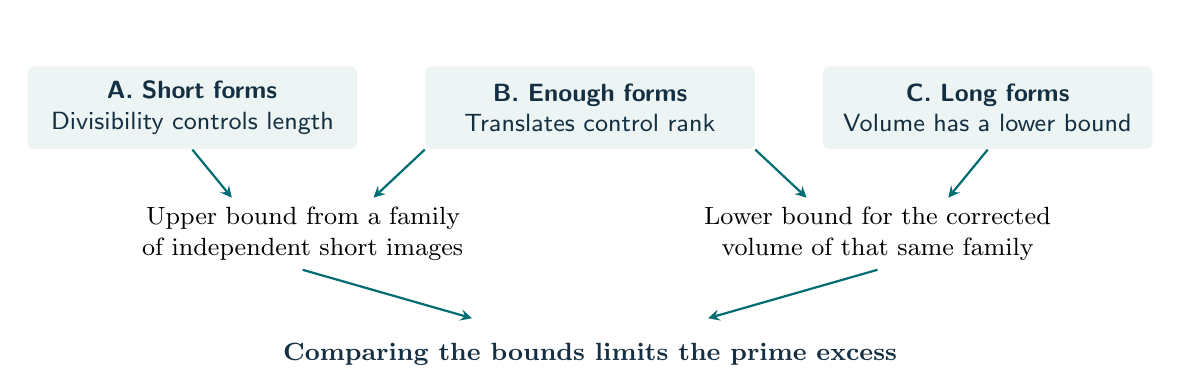
\begin{tikzpicture}[x=1cm,y=1cm,>=stealth, node distance=0cm,
 fact/.style={align=center, text width=3.95cm, minimum height=1.05cm,
              font=\small\sffamily, fill=pale, text=ink, rounded corners=2pt},
 result/.style={align=center, text width=5.0cm, minimum height=.9cm,font=\small},
 arr/.style={->,color=accent,thick}]
 \node[fact] (a) at (-5.05,2.65) {\textbf{A. Short forms}\\Divisibility controls length};
 \node[fact] (b) at (0,2.65) {\textbf{B. Enough forms}\\Translates control rank};
 \node[fact] (c) at (5.05,2.65) {\textbf{C. Long forms}\\Volume has a lower bound};
 \node[result] (up) at (-3.65,1.05) {Upper bound from a family\\of independent short images};
 \node[result] (lo) at (3.65,1.05) {Lower bound for the corrected\\volume of that same family};
 \node[result,text width=9cm, text=ink,font=\small\bfseries] (z) at (0,-.48)
   {Comparing the bounds limits the prime excess};
 \draw[arr] (a.south)--([xshift=-.9cm]up.north);
 \draw[arr] (b.south west)--([xshift=.9cm]up.north);
 \draw[arr] (b.south east)--([xshift=-.9cm]lo.north);
 \draw[arr] (c.south)--([xshift=.9cm]lo.north);
 \draw[arr] (up.south)--([xshift=-1.5cm]z.north);
 \draw[arr] (lo.south)--([xshift=1.5cm]z.north);
\end{tikzpicture}
\end{center}

\subsection*{Why introduce a chain?}
Let \(x\) be the point at which we want information about primes. The derivative data are set up so the logarithmic gain beyond the predicted divisibility contains a smoothed prime-counting error. Repeat the construction along \(m\) theta lifts. Each stage records a copy of the same error. An excess would shorten the images by an amount proportional to \(m\) times that excess in logarithmic units. The lower bound has to survive all \(m\) lifts as well. This is the difficult qualification behind the attractive idea of repetition.

Imagine the two calculations, after normalization to one dimension, taking the schematic form
\[
    H-E_{\rm low}\ \le\ V\ \le\ H-mD+E_{\rm up}.
\]
Here \(D\) is the excess, \(V\) the appropriately corrected log volume, and \(H\) a potentially enormous cost shared by the two calculations. Subtraction gives \(mD\le E_{\rm low}+E_{\rm up}\). If the lower estimate furnished only \(0\le V\), the upper estimate would instead give \(mD\le H+E_{\rm up}\), which can be useless. If \(E_{\rm low}+E_{\rm up}\) grew by another factor \(m\), division by \(m\) would give no improvement. In the actual proof there are also a rank fraction, a finite-place index and the normalizing weights of the prime sum. The precise cancellation and error sizes are derived in Section~\ref{sec:compare}.

An important surprise is \emph{how} the proof identifies \(H\). The upper calculation starts from factorials in derivatives and their prime divisors. The lower calculation starts from a Gram determinant for a succession of maps, factors it into determinants of individual lifts, and reads certain special \(L\)-values as norms of auxiliary forms. The number of distinguished factors in this second calculation reproduces exactly the number of ordinary directions in the first. Section~\ref{sec:one-lift-lab} derives the coefficient. Having the two calculations agree at their largest scale is what allows the much smaller prime discrepancy to be visible.

\subsection*{Where is the critical line in this picture?}
For a fixed progression and a fixed quadratic character, the quantity one ultimately bounds is a centered weighted sum \(R(x)\). Each prime power up to \(x\) has a coefficient proportional to \(1/n-1/x\). The weight is zero as \(n\) enters the sum and grows continuously as \(x\) increases. In this normalization the determinant calculation gives, at the level of powers of \(x\),
\[
                       R(x)\ \le\ x^{o(1)}/m .
\]
Here the displayed notation abbreviates the eventual upper estimates with arbitrarily small exponent loss obtained by making the auxiliary choices appropriately. A chain can be made of length about \(\sqrt{x}\) while its local errors are kept within budget. Thus the exponent furnished for \(R\) is \(-1/2+\varepsilon\), for every \(\varepsilon>0\).

To see why this is the right target, suppose a zero had real part \(3/4\). A term \(x^{-1/4+it}\) in a smoothed error would have a Mellin transform with a pole at \(3/4+it\) in the convention used here. For \(t\ne0\) its real part, \(x^{-1/4}\cos(t\log x)\), has positive peaks on the scale \(x^{-1/4}\), which exceeds \(x^{-1/2+\varepsilon}\) for \(\varepsilon<1/4\). This example predicts the contradiction but leaves two difficulties. The transform involves both original and twisted functions. A twisted real zero could supply a residue of the wrong sign, and coincident twisted zeros could cancel the pole one wants to detect. The proof removes those difficulties by choosing a quadratic twist in response to the hypothetical zero, checking the sign of all real residues in the half-plane of interest, and applying Landau's theorem to a positive measure. Section~\ref{sec:zero-detection} proves this implication without expanding the prime error as a sum over individual zeros.

One can now read the proof in either direction. Starting at the zeros tells us which sign and which exponent the arithmetic must deliver. Starting at the derivatives tells us why that sign and exponent are available. The two directions meet at a specific inequality for \(R(x)\). This is why a proof whose conclusion mentions only \(s\) and a Dirichlet character spends much of its length on lattices, projections, and the norm of an automorphic form.


\subsection*{Three theta functions a reader will meet}

The word \emph{theta} recurs at three very different scales in the argument. Recognizing which variable is being summed or differentiated makes their roles easier to follow.

\begin{center}\renewcommand{\arraystretch}{1.30}
\begin{tabularx}{\linewidth}{@{}>{\raggedright\arraybackslash}p{.24\linewidth}XX@{}}
\toprule
\textbf{What is summed} & \textbf{What one does to the sum} & \textbf{What it tells us}\\\midrule
An ordinary Gaussian on \(\mathbb Z\) &
Take a Mellin transform and use \(t\mapsto1/t\). &
The classical theta integral exhibits the reflection of completed zeta. Section~\ref{sec:firstpass}.\\
A lattice kernel depending on a pair of unitary groups &
Differentiate at specified places, integrate against a form, and compose the resulting maps. &
Prime powers determine divisibility. Norms of independent images turn that divisibility into an inequality. Sections~\ref{sec:weights}--\ref{sec:compare}.\\
A Gaussian weighted by a Dirichlet character &
Apply Poisson summation and average over quadratic twists of the character. &
Most auxiliary twists avoid zeros in one specified box, so a target zero remains visible. Section~\ref{sec:twist-mean}.\\\bottomrule
\end{tabularx}
\end{center}

The first calculation motivates reflection. The second supplies the prime estimate. The third makes the prime estimate answer a question about an individual zero. In particular, the \(L\)-values appearing in a formula for the norm of a unitary theta lift are auxiliary special values. The target \(L(s,\chi)\) at an arbitrary complex \(s\) appears in a different calculation, when the smoothed count is transformed back into logarithmic derivatives.

The order of choices matters just as much as the order of operations. Hand the proof a character and a possible zero. It can choose an auxiliary quadratic field suitable for that particular zero, then keep the field fixed. For every sufficiently large observation scale \(x\) it constructs new spaces of forms. Within a single such construction it may use a different auxiliary character to estimate a denominator at each coefficient prime. The resulting inequality concerns the same fixed quadratic field at all the observation scales. This is how local choices that vary from line to line of the proof can yield a global assertion about the character with which we began.

\section{What the half-plane theorem says}\label{sec:goal}
A Dirichlet character \(\chi\) modulo \(q\) is a multiplicative periodic function. It takes roots of unity on the classes coprime to \(q\), and is zero on the other classes. In the half-plane \(\Re s>1\), absolute convergence gives two descriptions of its \(L\)-function,
\[
  L(s,\chi)=\sum_{n\ge1}\frac{\chi(n)}{n^s}
    =\prod_p\bigl(1-\chi(p)p^{-s}\bigr)^{-1}.
\]
The Euler product gives nonvanishing here. Analytic continuation extends the function, with a pole at \(s=1\) for the principal character. The task is to continue the \emph{nonvanishing} far enough into the region where the Euler product no longer gives it. The theorem called \texttt{New.grh} accomplishes exactly this.
\keyeq{\Re s>\tfrac12,\qquad(\chi\ne\mathbf 1\ \text{or}\ s\ne1)
           \quad\Longrightarrow\quad L(s,\chi)\ne0.}
It applies to every integer modulus \(q\ge1\), including the character modulo one whose function is \(\zeta(s)\). For a primitive character the functional equation pairs its zeros in the open strip with zeros at \(1-s\) for the inverse character. For an induced character the extra finite Euler factors are nonzero throughout that strip, so the same pairing applies. Once the displayed theorem holds, these two zeros can both lie in \(\Re s\le1/2\) only if \(\Re s=1/2\). The zeta statement also singles out its trivial zeros at the negative even integers. Here GRH means the theorem for the entire family of Dirichlet characters. Higher-degree automorphic forms will enter as instruments in its proof.
\route{\sref{Statements}{statements}, \sref{New/Main}{functional equation}, \sref{Main}{the five exported theorems}}

\subsection{The arithmetic measurement}
Let \(Q\) be a multiple of \(18480\), choose a prime \(d\equiv Q/2-1\pmod Q\), and put \(\chi_d(n)=(n/d)\), the Legendre symbol. For each \(u\in\{1,Q\}\) set
\begin{align}
 \lambda_u(n)&=\mathbf1_{n\equiv1\pmod u}\,\Lambda(n)(1-\chi_d(n)),\nonumber\\
 R_u(x)&=\sum_{1\le n\le x}\lambda_u(n)\left(\frac1n-\frac1x\right)
               -\frac{\log x}{\varphi(u)}-c_u. \label{eq:remainder}
\end{align}
Here \(\Lambda(p^e)=\log p\) for \(e\ge1\), and \(\Lambda(n)=0\) otherwise. The fixed-modulus prime number theorem determines the constant \(c_u\) by \(R_u(x)\to0\). The weight \(1/n-1/x\) has a simple interpretation. It equals \(\int_n^x t^{-2}\,dt\). Thus \(R_u(x)+c_u\) is the integral from \(1\) to \(x\) of
\(t^{-2}(\sum_{n\le t}\lambda_u(n)-t/\varphi(u))\). The smoothing averages the discrepancy in the count. Its transform will retain the multiplicities of the zeros.

For example, for an inert prime \(p\) of \(\mathbb Q(\sqrt{-d})\), we have \(\chi_d(p)=-1\). Before restriction to a progression the powers \(p,p^2,p^3,p^4\) receive respective weights \(2\log p,0,2\log p,0\). Every power of a split prime receives zero, and each power of the ramified prime \(d\) receives \(\log d\). The same pattern will appear as the divisibility of a derivative.

The quantitative task is now precise. For every fixed admissible pair \((Q,d)\) and every \(\varepsilon>0\), prove that for all sufficiently large real \(x\),
\begin{equation}
                  R_Q(x)\le x^{-1/2+\varepsilon}.\label{eq:oneside}
\end{equation}
Only the upper side is required. This is an estimate for a smoothed remainder at a fixed modulus. The proof arranges the sign so that an excessively \emph{positive} remainder would force the determinant below its lower bound. Section~\ref{sec:zero-detection} explains why this one sign detects a zero of any Dirichlet character.

\subsection{What the three volume estimates say}\label{sec:contract}
Take independent vectors \(v_1,\ldots,v_n\). Their Gram matrix has entries \(\langle v_i,v_j\rangle\). Its determinant is the square of the volume they span. If each squared length is at most \(e^B\), Hadamard's inequality makes the log determinant at most \(nB\). In the simplest arithmetic model, if the columns form a square integer matrix \(A\) with nonzero determinant, that log determinant is also \(2\log|\det A|\ge0\). Every guaranteed common divisor removed from the columns reduces their lengths, but the resulting integral matrix still obeys this lower bound.

The actual target is a space of automorphic forms. The integral structures live on its lifts, can vary with a character, and come with denominators. Its lower bound has a large main term in place of zero. Three theorems provide what the integer example gets for free.
\begin{center}\renewcommand{\arraystretch}{1.17}
\begin{tabularx}{.97\linewidth}{@{}l X@{}}
\toprule
\textbf{Input}&\textbf{What it supplies}\\\midrule
A. Short forms & An upper bound on lifted lengths which decreases by \(m\) times a prime excess, with controlled denominators.\\
B. Enough forms & Independent short images spanning all but a small fraction of the target, using few translates.\\
C. Long forms & A lower bound on squared volume plus the cost of denominators for any such large family.\\\bottomrule
\end{tabularx}\end{center}
A zero map satisfies every upper bound on vector lengths. A lower bound in full dimension could miss a family which spans very few directions. The role of B is to make A and C apply to the same family.\route{\sref{New/Reduction/ShortAndEnough}{A and B}, \sref{New/Determinant/Twist/LongForms}{C}, \sref{New/Reduction/MainInequality}{their comparison}}

\section{Theta kernels, determinants, and a model pole}\label{sec:firstpass}
\subsection{What a theta kernel does}
One familiar theta series and one elementary matrix calculation explain the choice of tools. Begin with the Gaussian and sum its values over the integer lattice,
\[
       \vartheta(t)=\sum_{n\in\mathbb Z}e^{-\pi n^2t}\qquad(t>0).
\]
This single real function has both an arithmetic description and a symmetry. Its summands are indexed by integers; Poisson summation of the Gaussian gives
\(\vartheta(t)=t^{-1/2}\vartheta(1/t)\). Multiplying by \(t^{s/2}\) and integrating with respect to \(dt/t\) recovers an \(L\)-function. Indeed, for \(\Re s>1\), substitution \(u=\pi n^2t\) in each nonconstant term gives
\[
 \frac12\int_0^\infty \bigl(\vartheta(t)-1\bigr)t^{s/2}\frac{dt}{t}
       =\pi^{-s/2}\Gamma(s/2)\zeta(s).
\]
The factor \(1/2\) pairs \(n\) with \(-n\). Splitting this integral at \(1\) and replacing \(t\) by \(1/t\) in the lower interval gives the usual reflection symmetry of the completed zeta function. Reflection pairs two points in the strip. To place each zero \emph{on} the line, one also needs the half-plane exclusion of Section~\ref{sec:goal}.

In the construction below the theta functions have many variables. They also depend on two group elements \(g,h\). An integral against the first variable of a kernel \(K(g,h)\) sends a function \(F(g)\) on one quotient to a function of \(h\) on another. This operation is a \emph{lift}. As a linear operation it resembles a matrix with rows indexed by \(h\) and columns by \(g\). A large supply of symmetries of \(K\) makes the resulting function transform in the required way. A Taylor coefficient of \(K\) at a distinguished point retains arithmetic information from its lattice sum. The proof exploits both properties of the same kernel.

To see how one kernel can be studied in two orders, take finite sets \(I,J,K\), arrays \(A_{ji},B_{kj}\), input \(u_i\) and a test vector \(v_k\). Then
\[
 \sum_k\overline{v_k}\sum_j B_{kj}\sum_i A_{ji}u_i
   =\sum_j\left(\sum_k\overline{v_k}B_{kj}\right)
                 \left(\sum_i A_{ji}u_i\right).
\]
At left we tested an iterated lift. At right we can calculate by pairing the two inner expressions in the middle space. Genuine theta identities require compatible measures, period integrals, test functions and convergence. This finite equality explains the type of rearrangement that can turn a difficult norm or period into one amenable to computation. In Section~\ref{sec:weights} the two sides of a seesaw have identifiable advantages: derivatives on the definite side, and volume estimates on the other. The Gaussian calculation is background; the multivariable identity used for the bound is the \hyperref[sec:derivative]{seesaw identity} for these specific spaces.

\subsection{Dividing vectors and keeping the determinant}
For a nonzero integer \(D\), its real size is at least \(1\). With rational vectors, the same observation accounts for the cost of their denominators. Suppose \(Y\) is an invertible real \(n\)-by-\(n\) matrix with rational entries, and \(U\) is an invertible integer matrix such that \(YU\) has integer entries. Then
\[
  1\leq|\det(YU)|^2
   =\det(Y^{\mathsf T}Y)\,|\det U|^2
   \leq \left(\prod_i\|y_i\|^2\right)|\det U|^2,
\]
where \(y_i\) are the columns of \(Y\). Thus a large denominator can allow short independent columns. Keeping track of \(\log|\det U|\) restores a usable lower bound. If \(Y=\operatorname{diag}(1/3,1/5)\), take \(U=\operatorname{diag}(3,5)\). The logarithm of the squared covolume is \(-2\log15\), and twice the logarithmic cost of clearing denominators is \(+2\log15\). Equality holds. Clearing both columns by the same integer \(15\) would instead charge \(\log225\) for \(\log|\det U|\). The determinant records the individual costs.

Here is what changes in the proof. A column is a form. Its ambient norm comes from an integral or a class sum. Its integrality is measured at each prime and after certain twists. The short family may miss a few basis directions. Its reference logarithmic volume is a quantity \(H\) that grows with \(x\). The three accompanying estimates repair precisely these complications. A gives short vectors and the cost of making their lifts integral, B supplies enough directions, and C gives a lower bound for the corrected volume. Their common unit of comparison is a \emph{squared} volume, explaining both the factor \(2\) on denominator costs and the later coefficient at an inert prime.

\subsection{The analytic meaning of a half power}
There is also a quick way to anticipate the final exponent. A term \(x^{\rho-1}\), where \(\rho=\sigma+i\gamma\), has magnitude \(x^{\sigma-1}\) and oscillates as \(e^{i\gamma\log x}\). If one puts \(x=e^v\), its transform against \(e^{(1-s)v}dv\) is
\[
     \int_0^\infty e^{(\rho-s)v}\,dv=\frac1{s-\rho}
          \qquad(\Re s>\sigma).
\]
A zero of real part \(0.7\), for example, suggests an arithmetic disturbance with envelope \(x^{-0.3}\). A bound of order \(x^{-1/2+\varepsilon}\) for every \(\varepsilon>0\) is fine enough to detect this scale. This computation explains the target; it assumes neither an explicit formula summing over zeros nor the absence of cancellation between them. For the actual signed remainder only an upper bound is available. Section~\ref{sec:zero-detection} derives its transform, resolves the cancellations, and uses positivity to obtain the conclusion suggested by this simple pole.

\section{From counting points on a curve to counting prime powers}
\label{sec:discovery}

A question raised by the proof is how anyone would have thought to introduce a chain of unitary groups into a problem about primes. There is a clue in a proof of a different Riemann hypothesis. On a curve over a finite field, an auxiliary function can count points even when one cannot write down the points themselves. The trick is to design a function which spends a known amount of its total degree at every point one wants to count. Can one design an arithmetic object that spends a measurable amount at every prime one wants to count? The word \emph{spends} can be made precise in two different currencies. On the curve one counts orders of vanishing. In the number-field argument one compares divisibility at finite primes with the sizes of algebraic quantities at the complex embeddings. Alpöge identifies the passage between these problems as an inspiration for the proof. \href{https://alpo.ge/remark.pdf}{Alpöge, announcement, pp.~1 and 3--4.}

\subsection{How multiplicity pays for a point count}

Let \(C\) be a smooth projective curve over \(\mathbb F_q\). A nonzero rational function \(F\) on \(C\) has equal total orders of zeros and poles, counted over an algebraic closure. A bound on the poles is therefore a budget for the zeros. Suppose that the poles have total order at most \(D\), and that \(F\) vanishes to order at least \(M\) at each of \(N\) distinct rational points. Then
\[
                         MN\le D.
\]
At a smooth point with local parameter \(t\), requiring order at least \(M\) means that the coefficients of \(t^0,\ldots,t^{M-1}\) all vanish. This formulation works also when the characteristic divides a factorial. It makes visible two quite separate obligations. The vanishing conditions must hold, and the chosen function must survive them. The identically zero function would pass every local test and tell us nothing about \(N\). \href{https://numdam.org/item/SB_1972-1973__15__234_0/}{Bombieri, \emph{Counting points on curves over finite fields}.}

For a small example, work on the projective line over \(\mathbb F_7\) and consider
\[
                     F(T)=(T^3-1)^3 .
\]
The three nonzero squares \(1,2,4\) all solve \(T^3=1\). At such a root \(a\), the coefficient of \(u\) in \((a+u)^3-1\) is \(3a^2\ne0\). Hence \(F(a+u)\) begins with \((3a^2)^3u^3\), and the root spends exactly three units of degree. The only pole is at infinity. Substitution of \(T=1/t\) gives \(t^{-9}(1-t^3)^3\), so this pole has order nine. The bound \(3N\le9\) is attained. Cubing a given function multiplies its pole order and its zero orders by the same factor. The ratio stays at three. An effective use of multiplicity requires a construction in which the added vanishing is cheap relative to the pole order.

There is a specific resource in finite characteristic. At rational coordinates, replacing \(T\) by \(T^q\) preserves the value. In a local expansion at \(a\in\mathbb F_q\), however,
\[
                    (a+u)^q=a+u^q .
\]
The Frobenius variable is constant through orders \(1,\ldots,q-1\). For example, the expansion through degree \(<q\) of \(A(a+u)+(a+u)^q B(a+u)\) is that of \(A(a+u)+a B(a+u)\). This identity lets one impose conditions on jets at many rational points using common algebraic identities. A Stepanov construction uses functions and their Frobenius powers, a supply of coefficients, and an independent argument that the resulting function is nonzero. The pole budget must also be optimized. Stepanov's 1969 paper treats hyperelliptic curves over a prime field. Bombieri's subsequent account develops the method for general curves. These are square-root estimates in a geometric setting where the Frobenius map is available from the outset. \href{https://doi.org/10.1070/IM1969v003n05ABEH000834}{Stepanov, 1969}. \href{https://numdam.org/item/SB_1972-1973__15__234_0/}{Bombieri, Bourbaki seminar 1972--73, talk 430}.

\subsection{Why a point count can locate complex zeros}

The finite-field analogy has a second half. Suppose one has counted the points. How does the count say where the zeros are? For a smooth projective geometrically connected curve \(C\) of genus \(g\) over \(\mathbb F_q\), let \(N_n\) be its point count over the extension of degree \(n\). The zeta function packages all these counts in one rational function:
\[
 Z_C(T)=\exp\!\left(\sum_{n\ge1}N_n\,\frac{T^n}{n}\right)
     =\frac{P_C(T)}{(1-T)(1-qT)},\qquad
 P_C(T)=\prod_{j=1}^{2g}(1-\alpha_jT).
\]
Use the classical rationality and functional equation here as background. Comparing logarithmic derivatives at \(T=0\) gives the exact identity
\[
                       q^n+1-N_n=\sum_{j=1}^{2g}\alpha_j^n .
\]
If all \(|\alpha_j|=\sqrt q\), the error in the point count is at most \(2gq^{n/2}\). The converse is instructive. A bound \(|q^n+1-N_n|\le C_0 q^{n/2}\) for all \(n\) implies that
\[
  \sum_{n\ge1}(q^n+1-N_n)T^n
         =\sum_{j=1}^{2g}\frac{\alpha_jT}{1-\alpha_jT}
\]
is holomorphic for \(|T|<q^{-1/2}\). A reciprocal root \(\alpha_j\) with \(|\alpha_j|>\sqrt q\) would give a pole inside that disk. If the same \(\alpha_j\) occurs several times, its identical simple fraction is multiplied by a positive integer. Its residue cannot cancel. Thus each \(|\alpha_j|\le\sqrt q\). The functional equation pairs \(\alpha_j\) with \(q/\alpha_j\), so all these inequalities are equalities. Substitution \(T=q^{-s}\) takes \(|T|=q^{-1/2}\) to \(\Re s=1/2\). This gives a literal critical line behind the analogy. \href{https://math.mit.edu/~drew/BristolLecture1.pdf}{Sutherland, \emph{Computing zeta functions and \(L\)-functions}, lecture 1.}

For example, the elliptic curve \(y^2=x^3+x+1\) over \(\mathbb F_5\) has nine points. At \(x=0,1,2,3,4\), the right side is respectively \(1,3,1,1,4\), giving \(2,0,2,2,2\) square roots, and there is one point at infinity. The discriminant is nonzero modulo 5. For an elliptic curve \(\alpha_1\alpha_2=q\), while the point count just obtained gives \(\alpha_1+\alpha_2=5+1-9=-3\). Hence
\[
   P_C(T)=1+3T+5T^2,\qquad
   \alpha_{1,2}=\frac{-3\pm i\sqrt{11}}{2},\qquad
   |\alpha_1|=|\alpha_2|=\sqrt5 .
\]
As a check, \(\alpha_1^2+\alpha_2^2=9-10=-1\), so the same polynomial predicts \(N_2=25+1-(-1)=27\). A finite point count and the known genus-one functional equation suffice for this example. In higher genus more coefficients enter.

A comparison with the proof over the integers makes the new burden quite sharp. In the curve argument every \(\alpha_j\) enters a finite rational function with the same multiplicity sign, and the assumed error estimate is two-sided. For primes, the available determinant inequality is one-sided, and the continued transform contains the difference of two families of logarithmic derivatives. The quadratic-twist choice restores control over multiplicities near any proposed zero. Landau's theorem turns the one-sided bound and the signs on the real axis into holomorphy. The closing reflection has much the same purpose in the two arguments, though the route to its required half-plane exclusion is considerably longer for Dirichlet \(L\)-functions.


\subsection{A finite Fourier calculation that suggested a chain}
\label{sec:fourier-path}

Alpöge's discovery notes mention a sum on a path of variables. It can be read in two orders. One order detects the points of a quadric. The other lends itself to repeated applications of the same norm estimate. Here is the calculation with bounded scalar weights, so that both readings can be seen directly. This is a model of the observation in his notes. The arithmetic lifts used over the integers require different operators and different estimates. \href{https://alpo.ge/remark.pdf}{Alpöge, p.~3, footnote~3}.

Work over a prime field \(\mathbb F_q\). Set \(e_q(u)=\exp(2\pi i u/q)\), choose \(k\ge2\) functions \(t_j\) on the field with \(|t_j|\le1\), and form
\[
 Q(x_1,\ldots,x_k)=x_1x_2+x_2x_3+\cdots+x_{k-1}x_k.
\]
In this paragraph \(Q\) denotes the quadratic polynomial. Let \(N\) be the sum of the weights \(\prod_jt_j(x_j)\) over tuples satisfying \(Q(x)=0\). For \(h\in\mathbb F_q\) put
\[
 S(h)=\sum_{x_1,\ldots,x_k}\prod_{j=1}^k t_j(x_j)\ e_q\bigl(hQ(x)\bigr).
\]
Orthogonality gives \(\sum_h e_q(hu)=q\) for \(u=0\) and zero otherwise. Summing first over \(h\) thus gives \(\sum_h S(h)=qN\). Isolating \(h=0\) gives an exact second reading,
\[
 qN=\prod_j\left(\sum_x t_j(x)\right)+\sum_{h\ne0} S(h).
\]
A point count and a product of one-variable quantities have entered the same identity. For equal weights, the product is a \(k\)th power. The question becomes how rapidly the rest can grow with \(k\).

For \(h\ne0\) define the \(q\)-by-\(q\) matrix \(F_h(u,v)=q^{-1/2}e_q(huv)\). Its rows are orthonormal, by the same additive-character identity. Multiplication by \(t_j\) is a diagonal operator \(D_j\) of norm at most one. Expanding an ordinary matrix product along its intermediate indices gives
\[
 S(h)=q^{(k-1)/2}\, t_1^{\mathsf T}F_h D_2 F_h \cdots D_{k-1}F_h t_k .
\]
There are \(k-1\) Fourier matrices. Both end vectors have Euclidean norm at most \(\sqrt q\), including when the transpose at the left is written as a Hermitian pairing with \(\overline{t_1}\). Hence
\[
                |S(h)|\le q^{(k+1)/2}.
\]
A termwise absolute-value estimate gave \(q^k\). What changed was the decision to retain the common middle variable until its adjacent edges could be composed. The norm of a Fourier matrix is known exactly, however many times it is used.

Take three vertices and all weights equal to one. Then \(Q=x_2(x_1+x_3)\), and one can count directly. The branch \(x_2=0\) contributes \(q^2\) points, the branch \(x_3=-x_1\) another \(q^2\), and their intersection contains \(q\) points. Thus \(N=2q^2-q\). On the Fourier side \(S(0)=q^3\) and \(S(h)=q^2\) for every \(h\ne0\), since summing over \(x_1\) forces \(x_2=0\). In this example the bound on each nonzero frequency is attained. The example also shows exactly what the norm has left undecided. With general weights an individual frequency contribution can be complex. Even for real weights, the norm estimate alone supplies no sign for the weighted sum.

The author's analogy points to two separate resources. A path makes repeated norm estimates possible. Geometric information can put a sign on one side of a counting identity. Over the integers a theta lift occupies the place of an edge, and an arithmetic determinant supplies the constraint that a hypothetical prime excess would violate. The number-field theorem needs an estimate for the cost of each added edge. The simple fact \(\|F_h\|=1\) in the finite model explains why the actual norm and denominator computations, which occupy many modules, are essential to making the analogy work.

\subsection{What can play the part of multiplicity over the integers?}

There is no single characteristic in which to make this calculation for every rational prime. Each prime supplies its own reduction and its own Frobenius. The useful quantity here is a derivative of an algebraic theta value with controlled denominators. At a suitable inert prime \(p\), reduction of the theta expansion couples a variable to its partner under an odd power of Frobenius. The number of derivatives available in the two directions limits how often the coupling can occur. A term involving \(z^{p^e}w\), for example, consumes \(p^e\) units of degree in one variable for every unit in the other. If the budgets are \(a\) and \(b\), the excess beyond the second budget is measured by
\[
                   (a/p^e-b)_+
                  = a\,(1/p^e-1/x)_+,qquad x=a/b .
\]
Thus a positive part in a valuation estimate supplies precisely a smoothed cutoff on \(p^e\). The actual theorem allows other rows, other places, a ramified prime and error terms. The example explains why differentiating a theta function can reveal the same prime-power weight that occurs in a transform of logarithmic derivatives. \sref{New/Derivatives/Vacuum/Divisibility}{Local theta expansion}. \sref{New/Reduction/PrimeSums}{aggregation into prime sums}.

Suppose that the excess of such prime powers is positive and unexpectedly large. The resulting divisibility makes it possible to divide the constructed vectors by a large common factor. Their complex norms fall, subject to the cost of keeping their denominators under control. Why does this constrain the primes? A single vector can be tiny or zero. The proof produces translates whose span fills almost all of a specified target. From them one can extract independent vectors and take their Gram determinant. An upper bound comes from their individual lengths. An arithmetic lower bound comes from the product formula and the integral structures on the same forms. This is the additional reasoning behind the passage from the finite-field inequality \(MN\le D\) to a comparison of volumes. Independence plays the role formerly played by the proof that the auxiliary function is nonzero, and it supplies information in almost every target direction. \sref{New/Reduction/MainInequality}{The comparison on independent vectors}.

Taking a power of the \(\mathbb F_7\) example gave no improvement. Simply composing a map many times raises the same objection. Both its desirable divisibility and its unwanted growth can accumulate with the length. The construction therefore has to evaluate both sides with a common normalization. In the notation of Section~\ref{sec:compare}, the short-vector upper bound contains \(H-m\mathcal R\), and the lower volume estimate contains the same \(H\). The displayed terms are per direction, before the controlled errors. This coincidence is the point of computing the periods, level contributions and finite-place costs with such precision. If the lower bound reproduced only a fixed fraction of \(H\), an uncertainty of that larger order would remain after the subtraction. The accumulated term \(m\mathcal R\) can be isolated because the large parts match. \sref{New/UpperBound/Size/ArchimedeanSize}{Archimedean and finite normalizations}. \sref{New/Reduction/MainInequality}{final subtraction}.

\subsection{The obstruction recorded at two thirds}

Alpöge's discovery notes record an intermediate estimate suggesting a stopping point at exponent \(2/3\). He then describes putting different Hecke characters into a shared integral structure, exploiting approximate orthogonality, and controlling congruences between forms. He credits Claude with proposing about \(\sqrt{x}\) successive lifts for a prime sum of length \(x\). The exponent \(2/3\) here describes an intermediate calculation in the author's account of discovery. The theorem used in the finished proof is the determinant comparison in Section~\ref{sec:compare}. The useful mathematical question about the finished proof is which additional information makes so long a chain affordable. \href{https://alpo.ge/remark.pdf}{Alpöge, pp.~1 and 4, especially items~8--18.}

Consider what happens when a projection onto a chosen subspace introduces denominators. A favorable character at one rational prime may be quite unfavorable at a second. Requiring the same character to minimize every denominator would impose a simultaneous global selection problem. The seesaw identities relate the auxiliary calculations to a common untwisted determinant. One can then choose a character for the calculation at each coefficient place. Its powers must still satisfy all the conditions within that calculation. The determinant on which the product formula will act remains fixed. A scalar model illustrates the order of operations. If two representations of a positive rational number express it as \(D=r_1u_1=r_2u_2\), the valuation identity \(v_p(D)=v_p(r_i)+v_p(u_i)\) holds for either index. One may estimate the valuation at two primes using different identities, then combine the estimates for \(D\). Combining unrelated determinants would have no such justification. The cost of proving that appropriate identities and usable twists exist accounts for much of the Galois-theoretic part of the proof. \sref{New/UpperBound/Seesaw/SeesawIdentity}{The seesaw identity}. \sref{New/Congruences/FitTwistsExist}{simultaneous conditions at a coefficient place}.

There is a quantitative check on the proposed length. The local defect in the denominator calculation, expressed as a fraction of its allowed budget, has an upper bound of the form \(C m^2/(x(\log b)^2)\). At \(m\) between \(\sqrt{x}\) and \(2\sqrt{x}\), this contribution is at most \(4C/(\log b)^2\). Meanwhile the comparison buys a factor of \(1/m\) in the normalized prime discrepancy. One square root appears twice in these accounts. It is long enough to give a saving of \(x^{-1/2}\) in the quantity one wants, and short enough for the displayed cost to fit the budget. The proof still has to establish every other estimate and choose \(b\) so that the surviving powers of \(\log b\) cost at most \(x^\varepsilon\). This compatibility gives a mathematical reason for the choice of length, independent of its discovery story. \sref{New/Congruences/FitTwistsExist}{Denominator budget}. \sref{New/Reduction/OneSidedBound}{final dependence on the length}.

\subsection{Three ways to use symmetry or positivity}

Riemann's classical theta integral makes a particularly instructive comparison. Complete the computation in Section~\ref{sec:firstpass} by splitting the theta integral at one. With \(\Lambda_\zeta(s)=\pi^{-s/2}\Gamma(s/2)\zeta(s)\) the result is
\[
 \Lambda_\zeta(s)
 =\frac{1}{s(s-1)}
 +\frac12\int_1^\infty (\vartheta(t)-1)
           \bigl(t^{s/2}+t^{(1-s)/2}\bigr)\frac{dt}{t}.
\]
The rational term comes from integrating the constant terms introduced when \(t\) is inverted on \((0,1)\). The remaining integral converges for every \(s\) because \(\vartheta(t)-1\) decays exponentially at infinity. Both terms visibly stay the same under \(s\leftrightarrow1-s\). Reflection permits pairs of off-line zeros. For instance, for real \(0<a<1/2\) the polynomial \((s-a)(s-(1-a))\) satisfies the same reflection symmetry and has exactly such a pair. In the chain argument the theta kernels contribute arithmetic divisibility to a prime sum. Reflection enters again only once the right half of the strip has been cleared. The two appearances of theta thus carry distinct information. \href{https://www.claymath.org/collections/riemanns-1859-manuscript/}{Riemann's 1859 paper}. \sref{New/Main}{reflection in the readable proof}.

A spectral approach asks for a self-adjoint operator with the ordinates of \emph{all} nontrivial zeros as eigenvalues in the parameter \(s=1/2+it\). Self-adjointness forces those eigenvalues to be real. The difficult step is the correspondence with every zero. The method in this paper also uses spectra of operators, through Hecke eigensystems. Those spectra distinguish components of a space of forms and help calculate the index of a lattice. The zeros of the target Dirichlet functions enter via residues of logarithmic derivatives. The logical connection between these two appearances is a bound on a prime sum. It is possible to appreciate the role of the Hecke eigenvalues here without identifying any of them with a zeta zero. \href{https://www.claymath.org/library/monographs/MPPc.pdf}{Bombieri, official RH problem description}. \sref{New/Reduction/Zeros/PrimeError}{the residue computation}.

Finally, Weil's explicit-formula criterion converts RH into a sign condition on a quadratic functional for an entire class of test functions. This explains why a positivity identity can, in principle, settle a question about all the zeros. Here the initial determinant comparison delivers one side of a bound for a particular family of smoothed discrepancies. It comes with freedom to choose a quadratic twist after a proposed zero is specified. That choice prevents the twisted logarithmic derivatives from canceling the target pole. Positivity is used once more in a different variable. The upper bound on \(R_Q(e^v)\) permits the construction of a positive measure in \(v\). Landau's argument then constrains the real abscissa of its Laplace transform. The sign on the real axis controls an entire half-plane because absolute convergence there depends only on the real part. These mechanisms explain how the argument gets by with a one-sided prime estimate and why an \emph{arbitrary} one-sided bound would be inadequate. \href{https://doi.org/10.1070/IM1972v006n01ABEH001866}{Weil on explicit formulas}. \href{https://www.claymath.org/library/monographs/MPPc.pdf}{Bombieri on the sign criterion}. \sref{New/Reduction/Zeros/Criterion}{the criterion used here}.


\section{What earlier approaches made visible}
\label{sec:earlier}
Two successful theorems about RH illustrate the difference between finding a condition equivalent to the hypothesis and finding the estimate that decides it. One turns a zero into an obstruction to approximation. The other places the original zeta function at a particular time in an evolution. Each gives a precise question to put to the theta-lift proof. Where does the estimate come from? Why does it have the correct direction? These comparisons concern the mathematical statements in the cited papers. The account of how the chain was discovered comes from Alpöge himself.

\subsection{A zero that obstructs approximation}

Write \(u_a(x)=\{1/(ax)\}\) for \(a\) a positive integer, with braces denoting fractional part, and let \(e(x)=\mathbf1_{(0,1]}(x)\). Báez-Duarte's strengthening of the Nyman--Beurling criterion says that RH is equivalent to approximating \(e\) as closely as desired in \(L^2(0,\infty;dx)\) by finite linear combinations of the \(u_a\). Why should a question about fractional parts know anything about a zero? Their discontinuities encode the integers, and a Mellin transform reads them. \href{https://arxiv.org/abs/math/0202141}{Báez-Duarte, Theorem~1 (2003)}.

For \(0<\Re s<1\) one has
\[
 \int_0^\infty u_a(x)x^{s-1}\,dx=-a^{-s}\frac{\zeta(s)}s,
 \qquad
 \int_0^\infty e(x)x^{s-1}\,dx=\frac1s .
\]
For the first identity put \(v=1/(ax)\). On \((0,1)\), \(\{v\}=v\) contributes \(1/(1-s)\) before the factor \(a^{-s}\). On \([1,\infty)\), the formula
\[
 \zeta(s)=\frac{s}{s-1}-s\int_1^\infty \{v\}v^{-s-1}\,dv
\]
follows by partial summation for \(\Re s>1\) and continuation to \(\Re s>0\), away from \(1\). Adding the two integrals gives the claimed transform. Thus at a proposed nontrivial zero \(\rho\) the transform of any finite approximant vanishes, while the transform of its target is \(1/\rho\).

Here is the precise obstruction, including a small subtlety at infinity. Let \(g=e-\sum_a c_a u_a\), and suppose \(1/2<\sigma=\Re\rho<1\). On \((0,1)\), Cauchy--Schwarz bounds the transform by \(\|g\|_{L^2(0,1)}/\sqrt{2\sigma-1}\). On \((1,\infty)\) all the approximants have the simple shape \(1/(ax)\), so \(g(x)=B/x\) with \(B=-\sum_a c_a/a\). The transform of that tail is \(B/(1-\rho)\), and its \(L^2\) norm is \(|B|\). Applying Cauchy--Schwarz to these two contributions gives
\[
 \|g\|_{2}\ \ge\
 \frac{1}{|\rho|}
 \left(\frac1{2\sigma-1}+\frac1{|1-\rho|^2}\right)^{-1/2}>0 .
\]
This proves the direction we need for the comparison. An off-line zero would prevent approximation, whatever coefficients one chose. The half in this calculation is exactly where the square of \(x^{\sigma-1}\) becomes integrable at the origin. Proving that the distance actually tends to zero requires additional information.

The spanning theorem in the theta-lift argument also asks how well selected functions fill a space. Its target is a finite-dimensional space of automorphic forms depending on the desired prime-counting scale. The proof estimates pairwise overlaps of translates to fill a prescribed proportion of this target. It then uses the volume of independent columns as an arithmetic quantity. One might hope to read RH straight from the near-spanning statement. Its rank estimate alone says nothing about prime divisibility. The logarithmic lengths and their independent lower bound supply that missing information. The two occurrences of a Hilbert space thus lead to different concrete tasks. \sref{New/Reduction/ShortAndEnough}{Short vectors and near-spanning}. \sref{New/Reduction/MainInequality}{Where the rank estimate enters the determinant}.

\subsection{A deformation that puts the boundary at time zero}

In the de Bruijn--Newman approach, a rapidly decaying kernel \(\Phi\) from the completed zeta function defines
\[
 H_t(z)=\int_0^\infty e^{tu^2}\Phi(u)\cos(zu)\,du .
\]
The zeros at \(t=0\) are real precisely when RH holds. Differentiating under the integral yields \(\partial_tH_t=-\partial_z^2H_t\). In this family there is a threshold \(\Lambda_{\rm DN}\) such that all zeros of \(H_t\) are real precisely for \(t\ge\Lambda_{\rm DN}\). In particular \(\Lambda_{\rm DN}\le0\) is equivalent to RH. Rodgers and Tao established the other inequality, \(\Lambda_{\rm DN}\ge0\), by studying zero dynamics and the spacing of zeta zeros. The two inequalities answer distinct mathematical questions. \href{https://doi.org/10.1017/fmp.2020.6}{Rodgers and Tao (2020)}.

A two-root solution of the same differential equation shows what approaching such a threshold can mean. For an arbitrary real \(t_*\) set \(P_t(z)=z^2-2(t-t_*)\). Its derivative in \(t\) is \(-2\), and its second derivative in \(z\) is \(2\). For \(t>t_*\) its two roots are real. At \(t=t_*\) they meet, and for \(t<t_*\) they are purely imaginary. The existence of many times with real roots leaves the position of a designated time, such as zero, undetermined. This two-root calculation makes no assertion about a multiple zero of zeta.

The determinant proof can address time zero without estimating a zero trajectory. If \(H_0\) had a nonreal zero associated to a nontrivial zeta zero, reflection would give a zeta zero to the right of \(1/2\). The prime remainder and a suitable quadratic twist detect such a zero. The volume inequality excludes it. Combining the zeta conclusion with the threshold theorem and Rodgers--Tao immediately gives \(\Lambda_{\rm DN}=0\). This last sentence is a deduction from two results. The five exported theorems of the Lean package are listed in Section~\ref{sec:record}.

\subsection{Which step changes the strength of the estimate?}

Three uses of a square root can now be distinguished. In the approximation criterion it is a boundary of square integrability. For curves it is the size of a Frobenius eigenvalue required by the point-counting error. In the arithmetic construction it is a \emph{choice one gets to make}: how many lifts to perform for a sum of length \(x\). The first two identify where the answer should lie. The third explains how to gain a factor of that size. One still has to prove that the gain survives composition.

Alpöge describes precisely this issue in the discovery notes. He reports finding multiplicity two in an automorphic determinant and later encountering an apparent \(2/3\) barrier in the cost of the iterated lifts. He credits Claude with proposing a length on the scale \(\sqrt{x}\). These statements document a difficulty met in developing this proof. The earlier criteria above have different mathematical objectives. A useful way to read the rest of this guide is to watch for the two assertions that overcome the recorded difficulty. The upper estimate accumulates \(m\) copies of the discrepancy; the lower estimate matches the baseline of all \(m\) copies to the accuracy of the final error. Either assertion without the other would leave the choice \(m\simeq\sqrt{x}\) unexplained. \href{https://alpo.ge/remark.pdf}{Alpöge, pp.~1, 3--4}. \sref{New/Reduction/MainInequality}{The inequality used in the finished proof}.

\section{Building a residue class into a theta lift}\label{sec:weights}
Fix \(Q,d\). The remaining data vary with the large integer \(x\) at which we want to measure \(R_Q(x)\). First choose an imaginary quadratic field \(K=\mathbb Q(\sqrt{-d})\) and adjoin a root of unity to obtain \(E=K(\zeta_{q_1})\), where \(Q\mid q_1\). An infinite place of this CM field is a pair of complex-conjugate embeddings. Choosing the member extending one fixed embedding of \(K\) makes the set \(\Phi\) of places a copy of \((\mathbb Z/q_1\mathbb Z)^\times\). We can now give different derivative orders to embeddings according to their residue classes. Write \(f=|\Phi|\).
\begin{center}
\renewcommand{\arraystretch}{1.15}
\begin{tabularx}{.98\linewidth}{@{}l X@{}}
\toprule
\textbf{Choice} & \textbf{Role in the proof}\\\midrule
\(m\in[\sqrt{x},2\sqrt{x}]\) & Number of consecutive lifts, chosen to be a power of two.\\
\(r\in[x^5,3x^5]\) & Rank of the initial target hermitian space, a power of three. Put \(k=r+1-m\) and \(t=5r\).\\
\(x_1,b,a\) & Second cutoff, large weight, and derivative order. Here \(a=xb\) and \(x\ll x_1\ll b\).\\
\(A\subset\Phi\) & All places congruent to \(1\pmod Q\). They carry an extra derivative of order \(a\).\\
\(B\subset\Phi\) & Selected places congruent to \(-1\pmod Q\). The ordinary weight \(\kappa\) is \(b=a/x\) on \(B\) and \(a/x_1\) elsewhere.\\
\(M,N\) & \(M\) is a product of two level primes. The further prime level \(N\) offsets the archimedean cost of the long derivatives.\\\bottomrule
\end{tabularx}\end{center}
In the counting formulas $A$ and $B$ always denote sets of places. The construction proves both \(f=\varphi(Q)|A|\) and \(|A|/|B|\le\log b\). The second constraint leaves enough selected places to recover the desired remainder. Another constraint keeps \(B\) sparse along short strings of prime-power translates, controlling the occasions when large weights interact. These requirements can hold together. A Behrend construction chooses exponent vectors of equal squared length in a box. If a vector on that sphere is a strict weighted average of two other vectors on it, strict convexity forces all three to coincide. Encoding the vectors as digits without carries gives a large set of exponents avoiding the requisite congruences. The level primes are obtained in suitable progression windows. The existence theorem produces data for \emph{every sufficiently large integer} \(x\), so there is no passage from a sparse subsequence of test points.
\route{\sref{New/Reduction/Data/FieldsAndPlaces}{fields and places}, \sref{New/Reduction/Data/AdmissibleData}{parameters}, \sref{New/Reduction/Data/Existence}{existence}}

\subsection{Two derivative orders give two cutoffs}
Write \(z_+=\max(z,0)\). At place \(\tau\), the logarithmic divisibility counted by an order \(y\le a\) is represented by
\begin{equation}
 s_{\rm fin}(y,\tau)=\sum_{n\le a}\Lambda(n)(1-\chi_d(n))
             \bigl(y/n-\kappa(-n\tau)\bigr)_+ . \label{eq:sfin}
\end{equation}
The notation \(-n\tau\) denotes multiplication of \(\tau\) by the class of \(-n\) when this is a unit modulo \(q_1\). Otherwise the source uses the identity class. For \(y=a\), if the partner place belongs to \(B\), the positive part is \(a(1/n-1/x)_+\). At other places it is \(a(1/n-1/x_1)_+\). Thus the weight at an embedding determines how far into the prime-power sum that embedding sees.

Now sum over \(\tau\in A\). For each \(n\), exactly \(|B|\) of the partners \(-n\tau\) lie in \(B\) when \(n\equiv1\pmod Q\), and none do otherwise. For units this is just multiplication by a group element, together with the signs of the two residue classes. The formal statement covers the convention for nonunits as well. As a result one first counts every \(\tau\in A\) at the long cutoff \(x_1\). Then, precisely in the residue class of interest, one replaces \(|B|\) copies of that cutoff by the shorter cutoff \(x\). This finite counting identity is how a unitary-group construction singles out an arithmetic progression.

Put \(\log\bar\kappa=f^{-1}\sum_{\tau}\log\kappa(\tau)\) and define the expected value of the long-row sum and its excess by
\[
 s_{\rm main}=a\bigl(\log(a/\bar\kappa)+c_1\bigr),\qquad
 \mathcal R=\sum_{\tau\in A}\bigl(s_{\rm fin}(a,\tau)-s_{\rm main}\bigr).
\]
Expanding the two cutoffs with \eqref{eq:remainder} gives the exact identity
\begin{equation}
 \boxed{\displaystyle
 \frac{\mathcal R}{a}=|B|\bigl(R_Q(x)-R_Q(x_1)\bigr)+|A|R_1(x_1).}
 \label{eq:two}
\end{equation}
In detail, the uncentered sums contribute an additional
\(a\{|A|(\log x_1+c_1)+|B|\log(x/x_1)/\varphi(Q)\}\).
This equals \(|A|s_{\rm main}\) because of the two values of \(\kappa\) and the identity for \(f\). The two copies of \(c_Q\) cancel. This explains both the centering and the sign of the distant term in \eqref{eq:two}.
\route{\sref{New/Reduction/PrimeSums}{place count and the exact remainder identity}}

\subsection{Following one prime through both cutoffs}\label{sec:oneprime}
Take \(Q=18480\) and \(d=9239=Q/2-1\). Three primes illustrate how the two tests act independently. The second column gives the residue modulo \(Q\), and the third gives the quadratic character. The prime \(258721=14Q+1\) is \(29\bmod d\) and \(29^{4619}\equiv-1\pmod d\), so Euler's criterion makes it inert. The prime \(18481=Q+1\) is \(3\bmod d\), with \(3^{4619}\equiv1\pmod d\). The prime \(19\) is inert and fails the progression test.
\begin{center}
\begin{tabular}{@{}rrrrl@{}}
\toprule
\(p\)&\(p\bmod Q\)&\(\chi_d(p)\)&\(\lambda_Q(p)\)&Contribution before restricting the class\\
\midrule
\(18481\)&\(1\)&\(1\)&\(0\)&Zero at every power\\
\(19\)&\(19\)&\(-1\)&\(0\)&\(2\log19\) at each odd power\\
\(258721\)&\(1\)&\(-1\)&\(2\log258721\)&\(2\log258721\) at each odd power\\
\bottomrule
\end{tabular}
\end{center}
In fact, \(19\equiv-1\pmod5\) and \(5\mid Q\), so no odd power of 19 belongs to the desired progression. Every even power already has quadratic weight zero. Nevertheless an individual theta derivative can have a substantial 19-adic gain, as we will see in Section~\ref{sec:derivative}. It is the sum over places, and its comparison at two cutoffs, that selects the progression.

For \(p=258721\) define \(K_y(p)=(1/p-1/y)_+\). At this prime the sum of the raw long-row contributions over \(A\) is exactly
\[
  2a\log p\,\bigl[(|A|-|B|)K_{x_1}(p)+|B|K_x(p)\bigr].
\]
For an odd power \(p^e\) replace \(p\) in the kernel by \(p^e\), keeping \(\log p\). Each term has an unrestricted part \(|A|K_{x_1}\) and a correction \(|B|(K_x-K_{x_1})\) from the desired progression. In the variable \(u=1/n\), the graph of \(K_y(n)\) is a straight line of slope one after its threshold.
\begin{center}
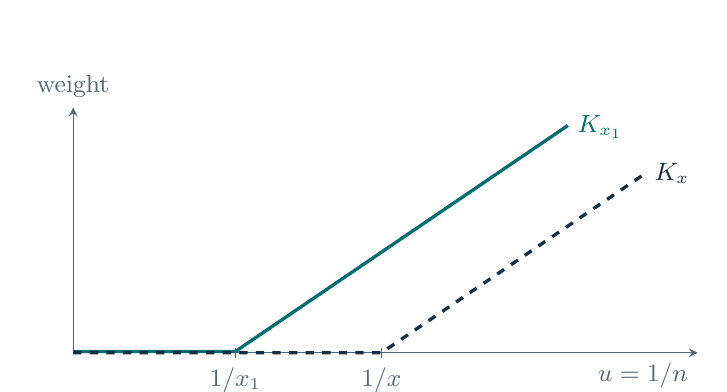
\begin{tikzpicture}[x=1.03cm,y=.70cm,>=stealth,every node/.style={font=\small}]
 \draw[->,quiet] (0,0)--(7.7,0) node[below left] {\(u=1/n\)};
 \draw[->,quiet] (0,0)--(0,4.45) node[above] {weight};
 \draw[very thick,accent] (0,.025)--(2,.025)--(6.1,4.125);
 \draw[very thick,ink,dashed] (0,0)--(3.8,0)--(7.05,3.25);
 \draw[quiet] (2,.09)--(2,-.10) node[below] {\(1/x_1\)};
 \draw[quiet] (3.8,.09)--(3.8,-.10) node[below] {\(1/x\)};
 \node[anchor=west,text=accent] at (6.1,4.1) {\(K_{x_1}\)};
 \node[anchor=west,text=ink] at (7.05,3.25) {\(K_x\)};
\end{tikzpicture}
\end{center}
When \(n<x\), the difference of the two kernels is the constant \(1/x_1-1/x\). When \(x<n<x_1\), only the longer kernel is positive. Beyond \(x_1\) both vanish. In particular the raw correction is nonpositive. The signed quantity \(\mathcal R\) can still be positive because it compares the total with its \emph{expected} value. It is an excess relative to this specified baseline that makes the normalized forms unusually short. The example uses an allowed fixed pair \(Q,d\) to illustrate the exact identities; in the zero argument the prime \(d\) will be chosen for a specified rectangle.

\subsection{Two routes to the same form}
A hermitian space over \(E\) is a vector space with a form that is linear in one variable and conjugate-linear in the other. Its unitary group preserves the form. An automorphic form here is, schematically, a function on an arithmetic quotient of such a group, with fixed transformation laws at the infinite and finite places. A theta lift integrates a form against a kernel built by summing a test function over rational vectors. In schematic notation, for groups attached to \(U\) and \(W\), it has the shape
\[
             f\longmapsto \left[h\longmapsto
                 \int_{[U]} f(g)\,\theta(g,h)\,dg\right].
\]
Conjugations, measures, test functions and level factors are fixed in the Lean construction. For definite spaces, the finite class-set description makes coefficients and their divisibility accessible.

There are two sequences of groups. The sequence based on \(X_0\) begins at rank \(k\) and adds \(t+1\) at each step. The sequence based on \(Y_0\) begins at rank \(r\) and adds \(t\) at each step. Since \(k=r+1-m\), the ranks at the last step differ by one, and \(Y_m\) sits inside \(X_m\). This inclusion permits restriction of a form there. The ranks count coordinates in a hermitian space. The dimensions of spaces of forms on the associated groups are different, usually much larger, numbers. At the other end a Poincaré series, a sum of translates of a prescribed function, gives a map \(\mathcal P\) from source forms on \(X_0\) to forms on \(Y_0\).

\begin{center}
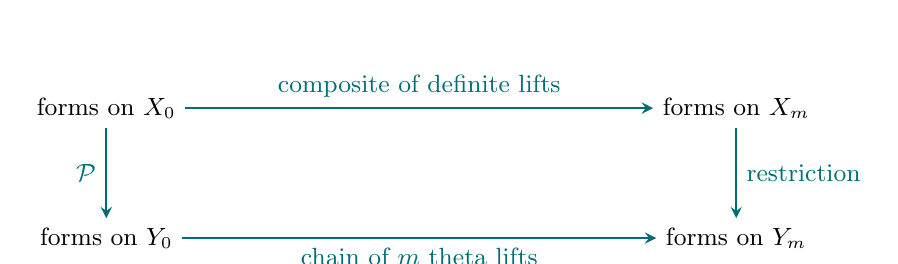
\begin{tikzpicture}[x=1cm,y=1cm,>=stealth, every node/.style={font=\small}]
\node (x0) at (0,1.65) {forms on \(X_0\)};
\node (xm) at (8,1.65) {forms on \(X_m\)};
\node (y0) at (0,0) {forms on \(Y_0\)};
\node (ym) at (8,0) {forms on \(Y_m\)};
\draw[->,thick,accent] (x0)--node[above]{composite of definite lifts} (xm);
\draw[->,thick,accent] (y0)--node[below]{chain of \(m\) theta lifts} (ym);
\draw[->,thick,accent] (x0)--node[left]{\(\mathcal P\)} (y0);
\draw[->,thick,accent] (xm)--node[right]{restriction} (ym);
\end{tikzpicture}\end{center}
The seesaw identity identifies the two outputs up to a fixed nonzero scalar, after taking the prescribed finite combination on the upper route and restricting to ramified source forms. The diagram suppresses twists and test data. One route exposes derivatives with controlled denominators. The other acts on a space whose determinant can be bounded. On \(Y_0\) a finite level group \(G\) acts. An idempotent \(e_0\) selects the local types used throughout. Its image is the target \(V\) of dimension \(d_T\). One may think of this projection as keeping prescribed symmetry types at the two level primes. Those types are chosen so that multiplicities can be compared between different unitary groups. Write \(\Theta_\xi\) for the lower chain on \(V\) with twist \(\xi\).
\route{\sref{New/UpperBound/Objects/Rows}{target}, \sref{New/UpperBound/Objects/Columns}{source}, \sref{New/UpperBound/Objects/RowChain}{chain}, \sref{New/UpperBound/Seesaw/SeesawIdentity}{seesaw}}

\section{How a theta derivative counts prime powers}\label{sec:derivative}

At the heart of the upper bound is a comparison one can already see for a polynomial. If a Taylor series $F(z)=\sum_j c_jz^j$ has $p$-integral coefficients, its $j$th derivative at zero is $j!c_j$. Thus differentiating guarantees at least $v_p(j!)$ factors of $p$. Legendre's formula expresses this valuation as $\sum_{e\geq1}\lfloor j/p^e\rfloor$. In a theta lift the Taylor series has partners in several variables, and its coefficients need not all be integral in the original coordinates. Accounting for both changes gives a different count, one that distinguishes splitting behavior and the weights at different places.

Fix the CM field $E$ of the construction and its imaginary quadratic subfield $K=\mathbb Q(\sqrt{-d})$. At a prime $p$ that does not split in $K$, the formal group of a CM elliptic curve gives a normal form for the theta Taylor series. After rescaling the variables, the series is an integral power series times an exponential. The possible denominators in that exponential are organized by expressions of the form
\[
  \Gamma_e(z)=\sum_{\tau,i}z_{\tau,i}^{p^e}z_{-p^e\tau,i}.
\]
Here $\tau$ indexes a place, $i$ indexes a coordinate, and $-p^e\tau$ denotes the partner place specified by the residue action. These pairs record the Frobenius action on the residue of a CM embedding, together with complex conjugation. They determine which two groups of variables can share a denominator. The contributing positive exponents are odd when $p$ is inert, and all positive exponents occur at the ramified prime $p=d$. An integral linear change of variables makes the relevant couplings sufficiently divisible in the degrees that a given derivative can see. The factorial valuation can then be applied. The chain rule charges a deduction when changing the variables back. The proof does this for derivatives defined by products of matrix minors, the polynomials describing the weights in a lift. \upperref{New/Derivatives/FormalGroup/ThetaProducts}{CM normal form} and \upperref{New/Derivatives/Divisibility/Count}{divisibility count}.

The resulting target for the valuation in a direction of order $y$ at $\tau$ has a simple expression. Write $u_+=\max(u,0)$ and let $\kappa$ be the weight on places. Put
\[
 s_p(y,\tau)=v_p(\pi_p)\sum_{e\in I_p}
             \bigl(y/p^e-\kappa(-p^e\tau)\bigr)_+.
\]
The index set $I_p$ consists of the positive contributing exponents just described. For split $p$, $I_p$ is empty. For inert $p$ the factor $v_p(\pi_p)$ is one, and for $p=d$ it is one half. These weights explain the exact prime sum when logarithms of \emph{squared} sizes are compared. If $p$ is inert then $1-\chi_d(p^e)$ is two for odd $e$ and zero for even $e$. At the ramified prime it is one for every $e\geq1$. Hence, for $0\leq y\leq a$,
\[
  2\sum_{p} s_p(y,\tau)\log p
  =\sum_{n\leq a}\Lambda(n)(1-\chi_d(n))
                  \bigl(y/n-\kappa(-n\tau)\bigr)_+
  =s_{\rm fin}(y,\tau).
\]
For a concrete local count take $Q=18480$, $d=9239$ and $p=19$. This prime is inert since $(19/9239)=-1$. Suppose its first and third partner places have the smaller weight $w=a/x_1$. For the trial order $y=2p^3w\le a$, the contributions at $p$ and $p^3$ are $721w$ and $w$ respectively. Already $y/p^5<w$, so higher powers contribute zero. Thus $s_{19}(y,\tau)=722w$ in this example. The positive part supplies the cutoff. Once $y/p^e$ has fallen below the partner weight, that prime power contributes nothing. The computation identifies the divisibility sought from a direction. Obtaining it for a chain of lifts requires controlling collisions in which two long rows occur at partner places. \upperref{Lib/CM/FormalGroup/PrimeNotation}{Local weights} and \upperref{New/UpperBound/Size/ShortColumns}{prime-by-prime gains}.

\subsection{Theorem A gives short forms at a controlled index}

The construction uses two descriptions of a vector on the final space $Y_m$. First send a source form $\phi$ on $X_0$ to a Poincar\'e series on $Y_0$, then apply the chain of $m$ theta lifts to $Y_m$. Alternatively, lift through the definite spaces $X_0,\ldots,X_m$, take a finite linear combination, and restrict to $Y_m$. An iterated seesaw identity equates the two descriptions on the ramified source space, up to a nonzero scalar independent of the twist. The definite description exposes the Taylor derivatives above. The $Y_0$ description is the one on which the lower determinant bound and the spanning argument operate. \upperref{New/UpperBound/Seesaw/SeesawIdentity}{Seesaw identity}.

The prescribed exponent $g(p)$ adds the contributions of the long rows of order $a$ at the $a$-places and the ordinary directions at all places, repeated through the $m$ lifts. At a collision a direct derivative count can lose some of this exponent at each step. The construction uses scaled Hecke operators at marked primes above exceptional $p$ to recover divisibility on a submodule. Bounds for the elementary divisors of those operators control the cost of restricting to it. The resulting estimate is simultaneous over twists of conductor prime to $p$. For each $p$ there is a nonnegative error $e_p$, with total $\sum_p e_p\log p\leq f a(\log b)^3$. On the indicated local submodule the composite lift has valuation at least $g(p)-e_p$. The colength, which measures the local index lost in passing to this submodule, is also controlled by $e_p$ times the dimension of the full source. This second assertion is what later permits arbitrary integral source forms to be used with a bounded correction to the index. \upperref{New/UpperBound/Divisibility/LocalDivisibility}{Local divisibility and colength}.

The factor $c_B=\prod_p p^{-\lfloor g(p)-e_p\rfloor}$ is a positive rational number with finite support in this product. Multiplying the map by $c_B$ spends the guaranteed finite-place divisibility to lower the complex size. In a squared norm its contribution is $2\log c_B$. On the complex side the cost assigned to a row of order $j$ is $s_\infty(j)=\log(j!)+j\log(M/\Omega)$, where $M$ is the product of the two level primes and $\Omega$ is the period scale. On the finite side one subtracts the prime sums just computed. The normalization of the period and the choice of the level $N$ account for the expected part of the long-row cost. The remaining signed contribution is minus $m$ times the excess $\mathcal R$ of the observed long-row prime sums over their expected values. A positive excess therefore produces shorter complex vectors.

More precisely, write $G$ for the finite level group, $\mathfrak p$ for the normalized projected Poincar\'e map, and $H$ for the main amount. The ramified source is spanned by globally integral $\phi$ satisfying, for every $s\in G$ and every complex field automorphism $\sigma$,
\[
  \bigl\|\Theta_1(s\mathfrak p\phi)\bigr\|_\sigma^2
       \leq \exp\{H-m\,\mathcal R+fa(\log b)^4\}.
\]
A target vector is integral at an identification $\iota:\mathbb C\simeq\overline{\mathbb Q}_\ell$ if, for every $m$-fold twist of conductor prime to $\ell$, its lift has integral coordinates there. An $m$-fold twist is one whose first $m$ powers remain ramified at each conductor place. To say a family has index at most $\delta$ means that, at each $\iota$, one matrix over the valuation ring makes its linear combinations integral simultaneously for all these twists. Its determinant has valuation at most $e_\ell$, where $\sum_\ell e_\ell\log\ell\le\delta$. If the members of a family belong to images of integral ramified forms under translates from a set $J$, the index allowance for that family is at most $2|J|\dim(S_{\rm ram})fa(\log b)^3$. In particular the number of translates used later has a measurable price. \upperref{New/Reduction/ShortAndEnough}{Theorem A, parts (a) and (b)}.

\section{Seeing an inert prime inside a derivative}
\label{sec:local-prime}

At which point does a derivative begin to distinguish a split prime from an inert one? One can see the first difference by differentiating polynomials with integer coefficients on a single elliptic curve. The full odd-prime-power pattern needs a second calculation with a formal parameter. Together these give a way into the local part of the proof.

\subsection{The same derivation at two primes}

Consider the affine elliptic curve \(y^2=x^3-x\) and its coordinate ring
\(A=\mathbb Z[x,y]/(y^2-x^3+x)\). The vector field dual to the differential \(dx/(2y)\) acts by
\[
 D(x)=2y,\qquad D(y)=3x^2-1.
\]
The derivative of the defining relation is zero, so these rules and the product rule give a derivation on \(A\). The curve has complex multiplication by \(i\), as one sees from the symmetry \((x,y)\mapsto(-x,iy)\), whose square is the negation map. The primes 3 and 5 are of good reduction. Modulo 3, the polynomial \(T^2+1\) is irreducible; modulo 5 it has the roots \(2,-2\). Thus 3 is inert and 5 splits in \(\mathbb Q(i)\). This curve illustrates the two reductions. In the global proof the imaginary quadratic field is \(\mathbb Q(\sqrt{-d})\) with a specially chosen prime \(d\).

Apply \(D\) three times, reducing each occurrence of \(y^2\) to \(x^3-x\):
\[
 D^3(x)=24xy,\qquad D^3(y)=60x^3-36x .
\]
Both vanish modulo 3. This already says something about \emph{every} function in \(A\). In characteristic \(p\) the \(p\)th iterate of a derivation is again a derivation, because the mixed binomial coefficients in the iterated product rule vanish. Since \(D^3\) kills the two generators modulo 3, it kills the entire ring modulo 3. Over the integers it follows that
\[
               D^a(A)\subseteq 3^{\lfloor a/3\rfloor}A .
\]
Indeed every additional block of three differentiations gives a factor of 3, and the derivatives are \(\mathbb Z\)-linear. An ordinary differential operation has imposed divisibility, uniformly over the input.

At 5 the same test gives a different answer. Continuing the recursion yields \(D^5(x)=(720x^2-144)y\equiv3D(x)\pmod5\). Using \(y=D(x)/2\) and the fact that \(2\) is a unit gives the same identity on \(y\). Since both sides are derivations modulo 5, \(D^5=3D\) on the entire reduced ring. Consequently \(D^{4j+1}(x)=3^jD(x)\bmod5\) for every \(j\ge0\). Arbitrarily long derivatives survive at this split prime. The contrast accounts for the first \(a/p\) in the inert-prime estimate recalled in Alpöge's announcement. The higher layers \(a/p^3,a/p^5,\ldots\) require more information than a calculation in characteristic \(p\) with one block of \(p\) derivatives. \href{https://alpo.ge/remark.pdf}{Discovery note, item~2}. \sref{Lib/CM/FormalGroup/PrimeNotation}{Prime decomposition and local rates in the proof}.

\subsection{Why the next layer is a cube of the prime}

A formal parameter \(T\) gives power-series coordinates near the identity of the CM elliptic curve. The analytic coordinate \(z\), in which the derivative is ordinary differentiation, and the parameter in which the group law is integral have different arithmetic normalizations. Fix an inert prime \(p\), and normalize its valuation by \(v_p(p)=1\). In the coordinate chosen in the formalization, put \(q_p=p^2\). Multiplication by \(p\) has the shape
\[
 T(pz)=g(T(z)),\qquad
 g(U)=pU+b_1U^{q_p}+\text{terms of higher degree},\qquad v_p(b_1)=0 .
\]
The power \(q_p\) in the first nonlinear unit coefficient is the feature of a height-two formal group that is relevant here. The series and the unit assertion are theorems for the source's particular CM curve and parameter.

There is a scale at which the two displayed terms have equal valuation. Choose \(\varpi^{q_p-1}=-p/b_1\), so \(v_p(\varpi)=1/(p^2-1)\). The precise rescaling theorem gives an integral series
\[
             Y(z)=T(\varpi z)/\varpi,\qquad
             Y-Y^{p^2}\equiv z\pmod p .
\]
It also gives the constant term zero. Iterating this congruence in formal power series, degree by degree, gives a particularly sparse answer,
\[
                Y\equiv z+z^{p^2}+z^{p^4}+z^{p^6}+\cdots\pmod p .
\]
Indeed the \(p^2\) power moves every exponent up by a factor \(p^2\) in characteristic \(p\). The tail eventually leaves any prescribed finite degree. The equality of the two valuations explains how the scale is chosen. Proving integrality of the rescaled coefficients is part of the formal-parameter theorem. \sref{Lib/CM/FormalGroup/FormalParameter}{Multiplication series and scaled parameter}.

The next calculation is about the theta function. After separating an integral factor, its rescaled Taylor series on one curve can be written
\[
 \theta(\varpi z)=W(z)\exp\!\bigl((\varpi^{p+1}/p)\,\Xi(z)\bigr).
\]
Here \(W,\Xi\) have integral coefficients. The local theta equation gives \(\Xi\equiv\lambda Y^{p+1}\bmod p\), where \(\lambda\) is a unit. The proof of this assertion isolates degrees in a particular congruence class in the logarithm of theta and proves a unit-coefficient statement. These are the elliptic-curve inputs. Once they are known, the odd powers can be read off by multiplying two sparse series:
\[
    Y^pY\equiv
       \left(\sum_{a\ge0}z^{p^{2a+1}}\right)
       \left(\sum_{b\ge0}z^{p^{2b}}\right) \pmod p .
\]
Each monomial has degree \(p^i+p^j\), with one index odd and the other even. Factoring out the lower power gives \(p^{\min(i,j)}(p^{|i-j|}+1)\). Their difference \(|i-j|\) is odd. Conversely every odd difference and every choice of the smaller index occur in this product. In particular the unshifted term \(z^{p^e+1}\) has a unit coefficient for every odd \(e\). This recovers the partner exponents from the CM curve's formal parameter. \sref{New/Derivatives/FormalGroup/Exponent}{Inert-prime exponent series and its unit coefficients}.

For a small instance of this local arithmetic, set \(p=3\), before imposing the global modulus conditions. The supports of \(Y\) and \(Y^3\) start with \(1,9,81\) and \(3,27,243\). Their product contributes the degrees below. Each entry is the sum of its row and column headings.
\begin{center}\begin{tabular}{@{}r|rrr@{}}
\toprule
&\(1\)&\(9\)&\(81\)\\\midrule
\(3\)&4&12&84\\
\(27\)&28&36&108\\
\(243\)&244&252&324\\\bottomrule
\end{tabular}\end{center}
For example \(28=3^3+1\), \(84=3(3^3+1)\) and \(252=3^2(3^3+1)\) all belong to the same partner difference \(e=3\). The degrees 4 and 244 exhibit \(e=1\) and \(e=5\). This table concerns the exponent of the local theta series. Exponentiating and changing variables again require estimates for factorials and denominators.

\subsection{From an odd difference to a smoothed prime count}

When one passes from one curve to the several variables in the lift, the two factors in a term of degree \(p^e+1\) acquire distinct place labels. The CM embeddings and their conjugates determine the pairing, and a resolution of the identity turns the sum of the terms into \(\sum_{\tau,c}z_{\tau,c}^{p^e}z_{-p^e\tau,c}\). Section~\ref{sec:inside-short} explains this passage. The multiplicity budgets of its two variables now need to be compared. If they are \(a\) and \(\kappa\), a coupling of this type uses \(p^e\) units of the first for one of the second. The positive excess is measured by \((a/p^e-\kappa)_+\). The local divisibility proof obtains this rate with the losses specified there.

Two identities show why this elaborate change of coordinates is worthwhile. At an inert prime the geometric series of unrestricted rates is
\[
 \sum_{e\ge1,\ e\ \mathrm{odd}}p^{-e}=\frac{p}{p^2-1}
              =\frac1{p-1}-\frac1{p^2-1}.
\]
On the right, the first term is the linear rate of \(v_p(a!)\); the second is the cost of the rescaling by \(\varpi\) per unit of degree. On the left, the same number has separated into layers at \(p,p^3,p^5,\ldots\). Thus two quite different readings of the local number agree. The unit coefficients in the exponent explain why nonzero interactions really occur at these layers. The eventual sharpness bounds for test derivatives address a further question about attaining the valuation after the other factors have been included. \sref{Lib/CM/FormalGroup/PrimeNotation}{Geometric series for the rate}. \sref{New/Derivatives/Sharpness/OneCurve}{Witnesses in specified derivative degrees}.

The second identity adds the cutoff, which a single asymptotic rate has lost. If \(\kappa=a/x\), then
\[
   (a/p^e-\kappa)_+=a\,(1/p^e-1/x)_+ .
\]
Taking squared norms pays \(2\log p\) per unit of inert-prime valuation. The resulting weights are exactly \(\Lambda(p^e)(1-\chi_d(p^e))\): twice \(\log p\) at odd powers, zero at even powers. At \(p=d\) the source has a different local expansion with all positive differences and a uniformizer of valuation \(1/2\). Its squared weight is \(\log d\). This local description is what makes it possible to recognize an analytic prime sum after aggregating many derivatives. A statement giving only the limiting slope \(p/(p^2-1)\) would discard which powers lie below \(x\).

\section{Inside the construction of a short form}\label{sec:inside-short}

The prime sum in Theorem A involves a single variable \(n\). Its source is a derivative in many variables, one group of variables for each embedding of a number field. We can follow a single summand through the construction. Its congruence condition comes from a permutation of the embeddings, its prime-power exponent from reduction of the theta function modulo a prime, and its sign in the final bound from dividing an algebraic vector by a rational number. The same normalization must work on a large enough family to constrain its volume.

\subsection{The places as a finite arithmetic construction}

Why are the places of \(E=K(\zeta_{q_1})\) suitable indices for variables? Fix a complex embedding of \(K=\mathbb Q(\sqrt{-d})\). Of the two conjugate embeddings of \(E\) that define a place, exactly one extends that embedding of \(K\). It sends \(\zeta_{q_1}\) to \(\zeta_{q_1}^{u}\) for a unit \(u\bmod q_1\). Every such unit occurs. Indeed, \(K\) embeds in \(\mathbb Q(\zeta_d)\), and the coprime conductors \(d,q_1\) give \([K(\zeta_{q_1}):K]=\varphi(q_1)\). This labels the variables by a group on which multiplication by a unit permutes them. Every prime divisor of \(q_1\) splits in \(K\), by the prescribed congruence for \(d\). In particular every prime power with nonzero coefficient \(\Lambda(n)(1-\chi_d(n))\) is a unit modulo \(q_1\). The formal convention for nonunits in \eqref{eq:sfin} therefore has no effect on the measured prime sum.

A small example illustrates the counting in \eqref{eq:two}. Take the units modulo \(25\), project to the units modulo \(5\), let \(A=\{1,6,11,16,21\}\), and choose \(B=\{4,9\}\) in the fibre over \(-1\). These small moduli illustrate the finite group calculation only. For two possible prime arguments, the partners, listed in the order of \(A\), are
\[
\begin{array}{c|ccccc|c}
 n&\multicolumn{5}{c|}{-n\tau\pmod {25},\quad \tau\in A}&\text{number in }B\\ \hline
 11&14&9&4&24&19&2\\
  2&23&13&3&18&8&0 .
\end{array}
\]
With trial cutoffs \(x=5,\ x_1=20\), the integer \(11\) is visible at the long cutoff and lies beyond the short one. Thus three of the five places contribute the factor \(1/11-1/20\), and two contribute zero, before multiplication by the common arithmetic weight and \(a\). In the second row there is no change of cutoff. The same reasoning counts any set \(B\) in the specified fibre, of any shape. The shape of \(B\) matters when a \emph{sequence} of partner places occurs in later estimates.
\route{\sref{New/Reduction/Data/FieldsAndPlaces}{cyclotomic irreducibility and splitting at the primes of the modulus}, \sref{New/Reduction/PrimeSums}{count at one integer}}

\subsection{How to keep many places while forbidding triples}

The size of \(B\) appears in the denominator when we solve \eqref{eq:two} for \(R_Q(x)\). The condition \(|B|\ge |A|/\log b\) makes that division affordable. At the same time the estimate that uses sparseness requires the following restriction. For each prime \(\ell\le kt\), write \(q_1^{(\ell)}\) for the largest divisor of \(q_1\) coprime to \(\ell\). Let \(s\) be given by \(2^s=m^{22}\) and let \(l_0\) be the least power of three strictly exceeding \(27s\). For \(0<i<j<l_0\) there must be no three members \(\sigma,\tau,\rho\) of \(B\) satisfying
\[
     \tau/\sigma\equiv\pm\ell^i,\qquad
     \rho/\sigma\equiv\pm\ell^j\pmod {q_1^{(\ell)}} .
\]
The signs are independent and repeated members count. This leaves a precise selection problem. Taking a single place would make the arithmetic signal too small. Taking the entire fibre would give many of the forbidden triples.

Here is the geometric fact used to solve it. For \(u,w\in\mathbb R^h\) and \(0<\lambda<1\),
\[
 \|(1-\lambda)u+\lambda w\|^2=(1-\lambda)\|u\|^2+\lambda\|w\|^2
                    -\lambda(1-\lambda)\|u-w\|^2.
\]
Consequently three points on the same sphere can satisfy a strict weighted-average relation only if they coincide. Among the \(H^h\) integer vectors of \(h\) digits in \(\{0,\ldots,H-1\}\), at most \(hH^2\) different squared lengths occur when \(h,H\ge1\). Some sphere therefore contains at least \(H^h/(hH^2)\) digit vectors. Read a vector on this sphere as an integer in base \(LH\), and let the modulus \(o\) be at least \((LH)^h\). If \(u_1,u_2,u_3\) are the resulting integers, a relation
\[
 (\alpha+\beta)u_2\equiv\alpha u_1+\beta u_3\pmod o,
 \qquad \alpha,\beta>0,\quad \alpha+\beta\le L
\]
forces an equality in each digit. Every digit on either side is smaller than the base, and both sides are below \(o\). Applying the identity for the sphere forces all three integers to coincide.

To see why a sphere says anything about prime powers, the source writes \(q_1=Q\cdot3l_0 2^s\) with \(2^s=m^{22}\). It sets \(g=1+3l_0 Q\), and uses the places represented by \(-g^u\) for selected exponents \(u\). All have the required sign modulo \(Q\). On a suitable power-of-two divisor of \(q_1\), \(g\) has order \(o=2^s\). For an odd prime \(\ell\), two forbidden ratios would imply
\[
       2j u_2\equiv 2(j-i)u_1+2i u_3\pmod o.
\]
Indeed, raising the first ratio to \(2j\) and the second to \(2i\) gives \(\ell^{2ij}\) in both cases and removes both signs. The sphere construction applies with \(L=2l_0\). If all three exponents coincide, the congruences still require \(\ell^{2i}\equiv1\) modulo a large power of two. The order bound in the construction gives \(2^s\le(\ell+1)2i\), contrary to its choice \(2l_0(kt+1)<2^s\). For \(\ell=2\) the argument instead uses the exact order of \(4\) modulo \(3l_0\). In this way a restriction covering all small primes follows from a single choice of exponents.

There is a separate elementary reason for the two primes in \(M=p_0p_1\). The lift needs an actual integer \(\alpha\in\mathcal O_K\) with \(\alpha\bar\alpha=M\). A split prime ideal can represent a nontrivial ideal class. If \(h_K\) is the class number, choose \(h_K+1\) distinct split primes in disjoint allowed windows, and write \((p_i)=I_i\bar I_i\). Two ideals, say \(I_i,I_j\), have the same class. Then \(I_i\bar I_j\) is principal, and its generator has norm \(p_i p_j\). For the other level prime \(N\), the field \(E\) contains \(\sqrt{-1}\), so a representation \(N=u^2+v^2\) supplies \(\pi_N=u+v\sqrt{-1}\) with \(\pi_N\bar\pi_N=N\). The prime-window input used to make these choices is of Siegel--Walfisz type. Its strength suffices because the construction allows the levels to be very large compared with the progression modulus.
\route{\sref{New/Reduction/Data/AdmissibleData}{definition of sparseness}, \sref{New/Reduction/Data/Existence}{sphere, powers of a unit, prime windows and norm generators}}

\subsection{What function is being differentiated?}

A theta kernel starts with a test function. The standard one used here, called the vacuum, combines a Gaussian at infinity with a twisted lattice indicator at the finite places. The theta function is obtained by summing over rational vectors. A scalar normalization makes the values of the standard vacuum at the specified finite translates integral at every prime and bounds their complex conjugates. Derivatives require additional control. An integral value at a point says little about the higher coefficients of the translated function there.

Complex multiplication supplies the link to a function of one variable. The elliptic curve attached to the lattice \(\Omega_0\mathcal O_K\subset\mathbb C\) has a theta function normalized at zero. A collection of vectors \(u_\nu\), with multiplicities \(b_\nu\), resolves the identity in the sense that
\[
                 z=\sum_\nu b_\nu(u_\nu^\dagger z)u_\nu.
\]
Here the dagger takes the conjugate transpose, and the equality uses the coordinates across the embeddings. The cyclotomic construction supplies such frames. For level-one standard data the Taylor series can, after the specified period scaling, be analyzed as a product of copies of the one-variable theta function along these linear forms, times a series in the corresponding local parameters. A formal group describes addition near the origin of the elliptic curve by power series. Its expansion controls precisely the part of the product capable of introducing denominators.

For an algebraic integer \(\alpha\in\mathcal O_E\), the two maps on either side of the following congruence agree at a nonsplit prime for each permitted exponent \(e\), giving
\[
              \tau(\alpha)^{p^e}\equiv\overline{\tau'(\alpha)}\pmod{\pi_p},
                    \qquad \tau'=-p^e\tau .
\]
All quantities are read in the chosen \(p\)-adic field. One can see the signs on the generators of \(E\). Raising \(\zeta_{q_1}^u\) to \(p^e\) gives exponent \(p^eu\), while complex conjugation negates the exponent at the partner. On the quadratic subfield, an inert prime has residue degree two. Frobenius acts there by the nontrivial conjugation, and its odd powers do the same. At \(p=d\), the generator \(\sqrt{-d}\) is zero modulo \(\pi_p=\sqrt{-d}\). The quadratic condition then allows every exponent, including zero. Thus a distinction visible on just two generators dictates the permitted interactions of all the Taylor variables.

Write \(L_\nu(z)=u_\nu^\dagger z\). The following polynomial would ordinarily involve the coefficients of every \(u_\nu\). Reduction modulo \(\pi_p\) gives
\[
       \sum_\nu b_\nu L_\nu(z)^{p^e} L_\nu(z)
       \equiv \sum_{\tau,c} z_{\tau,c}^{p^e}z_{-p^e\tau,c}=\Gamma_e(z)
       \pmod{\pi_p}.
\]
The power of a sum in characteristic \(p\) distributes over its terms. The congruence on coefficients moves the surviving coefficient to its partner, and the resolution of the identity then returns the corresponding coordinate. This explains why the result depends on a permutation of places, even though the lattice vectors used to describe the theta function may look quite different.

For the normalized series \(F\) of such data, the precise conclusion has the form
\[
   F(\varpi z)=W(z)\exp\!\left(
       \frac{\varpi^{p+1}}p\sum_{e\in I_p^\circ}\sum_{j\ge0}
                                  \lambda_{ej}\Gamma_e(z)^{p^j}\right).
\]
Here \(W\) has \(p\)-integral coefficients, each \(\lambda_{ej}\) is integral, \(I_p^\circ\) includes zero only for the ramified prime, and \(v_p(p)=1\). The change of scale has \(v_p(\varpi)=1/(p^2-1)\) in the inert case and \(1/(2p-2)\) in the ramified case. The displayed exponential is a formal power series. At any fixed total degree only finitely many of the displayed powers can contribute. The theorem turns a question about all coefficients of a multivariable theta function into a question about the specified monomials in \(\Gamma_e\).
\route{\sref{New/Derivatives/Vacuum/IntegralVacuum}{integral vacuum and theta products}, \sref{New/Derivatives/FormalGroup/ThetaProducts}{congruence and resolution of the identity}, \sref{New/Derivatives/Vacuum/Divisibility}{normal form for the Taylor series of standard data}}

\subsection{Reading a prime-power term out of a diagram}

For a polynomial \(P\) in the matrix entries, a \emph{jet} here means the number \(P(\partial)F(0)\). For example, the determinant of a two-by-two block gives the differential operator \(\partial_{11}\partial_{22}-\partial_{12}\partial_{21}\). A column of height \(h\) prescribes a minor of order \(h\). Multiplying the minors gives one of the differential operators used to read the lift. As a small example, a diagram with two columns of height one and a column of height two can prescribe
\[
          P(Z)=Z_{11}^2(Z_{11}Z_{22}-Z_{12}Z_{21}).
\]
Every term has degree four. Applying it to a power series gives a signed sum of factorials times coefficients of degree four. The alternating determinant enforces the prescribed transformation under change of coordinates. In the lift, a place in \(A\) contributes \(a\) columns of height one to the diagram, forming its long row. At other places this contribution is absent. Additional columns, beginning at height \(k\), encode the ordinary directions.

One monomial explains the positive parts in the valuation formula. A term \(z^{p^e}w\) used \(h\) times requires at least \(hp^e\) derivatives in \(z\) and \(h\) in \(w\). If the two available degrees are \(y\) and \(v\), its possible occurrences number at most \(\min(\lfloor y/p^e\rfloor,v)\). The algebraic identity
\[
                 y/p^e-\min(y/p^e,v)=(y/p^e-v)_+
\]
shows how much of a factorial contribution of size \(y/p^e\) survives a deduction of that form. Several couplings can occur together, and a minor differentiates several coordinates at once. The actual proof chooses directions that make the requisite couplings divisible in the degrees being tested, applies the multivariable factorial inequality there, and calculates the cost of this substitution upon returning to the original variables.

The statement for one diagram makes the distinction between a requested gain and a proven valuation concrete. At each place let \(t_\tau\) count columns of height one, \(c_\tau\) count the remaining columns of height below the row cutoff, and \(u_\tau\) count their boxes. For positive \(e\in I_p\) the summand at \((\tau,e)\) of the predicted exponent before the factor \(v_p(\pi_p)\) is
\begin{equation}
 \left(\frac{t_\tau}{p^e}-t_{\tau'}-c_{\tau'}\right)_+
 +\left(\frac{u_\tau}{p^e}-u_{\tau'}\right)_+
 -\frac{c_\tau}{p^e},\qquad \tau'=-p^e\tau.\label{eq:short-diagram}
\end{equation}
At \(p=d\) there is a further subtraction, half the sum over \(\tau\) of
\(\min(t_\tau,t_{\tau'}+c_{\tau'})+c_\tau+\min(u_\tau,u_{\tau'})\) for \(\tau'=-\tau\). This is the trace of the exponent \(e=0\) in the Taylor formula. If \(n'\) is the number of rows and \(b_*\) is the total number of boxes counted, the theorem bounds the valuation below by this prediction less
\(f(n')^3(1+\log_p\max(b_*,1))\). The logarithmic loss includes the digit errors that arise when estimating factorial valuations in many variables. Replacing these detailed counts by the simpler weight \(\kappa\) gives the requested sum of Section~\ref{sec:derivative} with a controlled error. In particular the local identity with \(\Lambda(p^e)(1-\chi_d(p^e))\) concerns the requested gain. Equation~\eqref{eq:short-diagram} explains the work needed to obtain that gain to sufficient accuracy.
\route{\sref{New/UpperBound/Objects/Weights}{columns of the lift diagrams}, \sref{New/Derivatives/Divisibility/Count}{jet theorem for products of minors}, \sref{New/UpperBound/Divisibility/JetExponent}{comparison with the requested exponent}}

\subsection{Following a vector through the seesaw}

There are two reasons for changing groups in the middle of the argument. The definite groups permit a finite description of their forms by lattice classes. The group of the original target \(Y_0\) has the signatures and distinguished periods needed for the comparison with the lower bound. At stage \(j\) the difference in ranks is
\[
       \dim_E Y_j-\dim_E X_j=m-1-j.
\]
For \(j<m\), the Gram matrix on \(Y_j\) contains the positive form on \(X_j\) and an additional block of this length. Its off-centre coordinates form hyperbolic pairs, with Gram matrix \(\left(\begin{smallmatrix}0&1\\1&0\end{smallmatrix}\right)\), and its middle entry, when present, is \(-N\). At \(j=0\) there are \((m-2)/2\) pairs and one middle coordinate. Moving one step along the chains shortens the block by one. At \(j=m-1\) it has disappeared, and at the final stage the direction of inclusion reverses. The standard definite \(Y_m\) is a codimension-one subspace of the standard definite \(X_m\).

To identify the forms on \(Y_m\), pair the lower-chain output with a test form there. Unfolding the Poincar\'e series rewrites this pairing as an integral over a subgroup against a prescribed character, called a Bessel period. In one step of the seesaw the theta kernel transfers that period through the lift. The outer integration splits into an archimedean integral and a weighted sum over finite classes. Repeating the step with the shorter additional block leaves a pairing of a definite lift with the test form on the codimension-one subspace. This supplies the restriction at the top. The finite weights arising from the subdivision into classes have controlled denominators. After the required normalization, primes away from the conductor of the twist preserve their integrality. This control over the coefficients is essential to carry the jet bounds through the identity.

More explicitly, for fixed evaluation data in the Poincar\'e series there exists \(c_{\rm ss}\ne0\) such that, for each permitted twist \(\xi\), a finite collection of coefficients \(\Psi_\xi\) gives the following identity for every ramified source form \(\phi\).
\[
  \Theta_{\xi}^{\rm raw}\,\mathcal P\phi
       =c_{\rm ss}\,B_{\xi,\Psi_\xi}\phi.
\]
Here \(\Theta_{\xi}^{\rm raw}\) is the chain on principal-level forms before projection to the selected target, and \(B_{\xi,\Psi_\xi}\) denotes the finite combination of definite chains with their final restriction. The same scalar works for all the twists. Their finite coefficient families may differ. This identity transfers size and divisibility of the definite expressions to the Poincar\'e images. Independence of those images requires a rank estimate, given in Section~\ref{sec:span}.

What makes the adjective \emph{ramified} operational here? At each of the \(f\) primes \(w\mid\pi_N\), a local scaling acts by an operator \(Z_w\) with \(Z_w^{N-1}=1\). The ramified source is the space on which each \(1+Z_w+\cdots+Z_w^{N-2}\) vanishes. On a complex eigenvector of \(Z_w\), the geometric sum acts by \(N-1\) if the eigenvalue is one and by zero at every other \((N-1)\)-st root of unity. Hence the space is the image of \(\prod_{w\mid\pi_N}(1-Z_w)\), as the scalings commute. This description avoids dividing by \(N-1\) when constructing integral forms in the subspace.

How expensive is that restriction? A vector fixed by \(Z_w\) is fixed by the larger level obtained by adjoining this scaling. The index of the original level there is at least \(N-1\). At the free levels in this argument the dimensions are proportional to the corresponding class counts, so at most \(1/(N-1)\) of the source dimension is fixed. Summing the bounds for the kernels of the differences gives
\[
      \frac{\dim S-\dim S_{\rm ram}}{\dim S}\le\frac f{N-1}\le b^{-8}
      \quad (\dim S>0).
\]
The free-level description also supplies short spanning vectors. One can specify a vector at one lattice class at a time, and use the integral weight polynomials there. Under a single difference \(1-Z_w\), integrality persists, and two vectors of squared size at most \(C\) have difference of squared size at most \(4C\). Thus applying all the differences increases this starting bound by at most \(4^f\). The estimates for the lift absorb that cost. Both size and dimension have now been quantified before choosing a single independent target image.
\route{\sref{New/UpperBound/Objects/Rows}{Gram matrices of the lower spaces}, \sref{New/UpperBound/Seesaw/SeesawIdentity}{iterated period transfer}, \sref{New/UpperBound/Size/ShortColumns}{scalings, dimension and short vectors}}

\subsection{Repairing a collision without paying for it at every step}

Inspect the first positive part in \eqref{eq:short-diagram}. At a long row \(t_\tau=a\), a second long row at its partner gives \(t_{\tau'}=a\). It can erase the whole contribution from that term. Such a pair \(\tau,\tau'\in A\) is a \emph{collision}. For a contributing prime, \(p\) is a unit modulo \(Q\), so its occurrence requires \(p^e\equiv-1\pmod Q\). A partner in \(B\) changed an ordinary weight and selected the desired progression. Collisions involve two long rows in \(A\), whose definition fixes the entire fibre, leaving no freedom to remove them from the design.

In one lift the unpaid amount from a collision is bounded by \(a/p^e\). Write \(C_p\) for the sum of these bounds over the collision pairs, and \(g_p\) for the requested exponent over all \(m\) lifts. Applying the single-lift estimate \(m\) times yields a bound of the form \(g_p-\mathcal L_p-m C_p\), where
\[
       \mathcal L_p=\frac{fa(\log b)^2}{p}
       \begin{cases}m,&p\equiv\pm1\pmod m,\\1,&\text{otherwise}.\end{cases}
\]
For a nonexceptional nonsplit prime below \(x_1\) the congruences and decay of \(p^{-e}\) give \(m C_p\le\mathcal L_p\). The exceptional case is an inert prime \(p\not\equiv\pm1\pmod m\) for which the multiplicative order of \(-p\) modulo \(Q\) is odd and at most \(\lceil\log_p m\rceil\). Here a small exponent can cause a recurring collision, and this argument alone gives too large a loss.

Fix a \(p\)-adic embedding. The places in a colliding pair induce conjugate primes in the construction at an exceptional \(p\). Choose one prime from every relevant conjugate pair. This is a full mark. A Hecke operator at a marked prime is a finite correspondence given by a sum of translates. Scaling it by the prescribed power of \(p\) gives an operator on integral source forms. Write \(U\) for the product of these scaled operators, \(M_p\) for the local module of integral source forms, and \(j_p=\lceil 2mfa/p\rceil\). Moving these operators through the lifts supplies divisibility for the rows at the marked places. Every collision meets a marked side, and the valuation bound on \(U^m M_p\) becomes \(g_p-2\mathcal L_p\). The same bound holds on \(p^{j_p}M_p\) by the crude estimate \(m C_p\le j_p\). It therefore holds on their sum.

It matters how large this sum is. For a model over \(\mathbb Z_p\), suppose an integral matrix has elementary divisors \(p^{s_1},\ldots,p^{s_h}\). In diagonal coordinates its image plus \(p^j\mathbb Z_p^h\) has index \(p^{\sum_i\min(s_i,j)}\), since in coordinate \(i\) the two generators are \(p^{s_i}\) and \(p^j\). For instance the exponents \((0,0,7)\) and \(j=3\) cost three powers of \(p\) in total. Multiplying every coordinate by \(p^3\) would cost nine. The elementary-divisor estimate proved for these Hecke operators plays exactly this role. In the formal module's index sense it bounds the cost of \(U^m M_p+p^{j_p}M_p\) by \(\mathcal L_p\dim S\) powers of \(p\). Intersecting with the ramified source gives a submodule on which the required gain holds simultaneously for every permitted twist of conductor prime to \(p\).

Finally one sums over primes. Away from the small nonsplit primes and from \(N\), the gain and loss are zero and the chain preserves integrality. The level prime \(N\) has its own loss estimate. Writing \(e_p\) for the combined losses, the formal bound is \(\sum_p e_p\log p\le fa(\log b)^3\). Multiplication by \(p^{-\lfloor g_p-e_p\rfloor}\) leaves the local output integral on the indicated submodule. The loss from rounding each exponent down is less than \(\log p\) in the ordinary logarithmic size, and the sum of these \(\log p\)'s over the support is at most \(b\). Thus the single rational scalar used across all primes satisfies
\[
       \log c_B\le -\sum_p g_p\log p+fa(\log b)^3+b.
\]
The factor in a squared complex norm is \(\exp(2\log c_B)\) at every conjugate because \(c_B\) is rational. The local submodules need not have the same basis. Their costs enter the index estimate of Theorem A, while the single complex normalization transfers the measured prime excess to the lengths of the lifted vectors.
\route{\sref{New/UpperBound/Divisibility/JetExponent}{cost per collision}, \sref{New/UpperBound/Divisibility/LocalDivisibility}{marked operator, corrected module and uniform divisibility}, \sref{New/Reduction/ShortAndEnough}{rounding, normalization and the two conclusions of Theorem A}}

\section{Why few translates span almost the whole target}\label{sec:span}

A short vector gives no constraint if all the maps send it to zero. Many copies of one short direction would also be insufficient for a lower bound involving the target dimension. Theorem B proves the necessary independence by measuring overlaps between translates. For this argument let $P$ denote the Poincar\'e map with its second-moment normalization on the \emph{full} source, of dimension $h$. Let $e_0$ be the orthogonal projection onto the target of dimension $d_T$, and write $s$ for the unitary action of a member of $G$. For an operator $A$, $\|A\|_{\rm HS}^2$ is the sum of $\|A v_i\|^2$ over an orthonormal basis. The overlap of $P$ with its translate $sP$ is measured by $P^*sP$.

Two estimates carry the analytic work. For each subspace $U$ of the full source,
\[
 \|e_0P\operatorname{pr}_U\|_{\rm HS}^2
           \geq \dim U-5b^{-4}h,
 \qquad
 \frac{d_T}{|G|}\sum_{s\in G}\|P^*sP\|_{\rm HS}^2
           \leq (1+9b^{-4})h^2 .
\]
The first excludes loss of a large subspace through projection onto the selected local types. The second bounds the average squared overlap. To prove the estimates one unfolds the inner products of Poincar\'e series into sums over pairs of rational elements with prescribed congruences. The main terms are controlled by local orbital integrals, Poisson summation and a sieve over places. The other terms are bounded by counting lattice frames with fixed congruences and discriminants. A dimension estimate for the target uses equality of relevant multiplicities with a definite unitary space where the level is free and the dimension can be counted. \upperref{New/Spanning/Unfolding/Moments}{Unfolded moments} and \upperref{New/Spanning/SecondMoment/SpanningTheorem}{normalized estimates}.

The first estimate puts nearly one unit of squared norm into the selected target per source dimension. The second prevents too much of that norm from lying in the directions already occupied by earlier translates. Estimating this overlap and iterating gives the following quantitative conclusion. 
\[
 |J|\dim S_{\rm ram}\leq 5d_T\log(1+2b^2),\qquad
 \dim\sum_{s\in J}s\mathfrak p S_{\rm ram}
           \geq(1-4/b^2)d_T>0
\]
for a suitable finite $J$ and the large admissible parameters. Because the forms supplied by Theorem A span their source and work for every translate at once, a basis of this sum can be chosen from their images. These are the vectors whose Gram determinant is compared with the lower bound. \upperref{New/Spanning/SecondMoment/FewTranslates}{Finite-dimensional argument} and \upperref{New/Reduction/ShortAndEnough}{Theorem B}.

\subsection{A cyclic example in which all the overlaps can be counted}
\label{sec:cyclic-frame}
The factor $1/d_T$ in the mean overlap bound has a geometric meaning. To see its value before dealing with automorphic forms, take a $d$-dimensional space with orthonormal coordinate vectors $e_0,\ldots,e_{d-1}$, indexed cyclically. Let $P$ include the span of the first $h$ coordinate vectors, where $1\le h\le d$, and let the $d$ shifts act by $s e_i=e_{i+s}$. The matrix entry in position $(i,j)$ of $P^*sP$ is $1$ when $i=j+s\pmod d$ and is zero otherwise. Its squared Hilbert--Schmidt norm counts exactly the ordered pairs $(i,j)$ of indices in the original block having difference $s$. Each of the $h^2$ pairs supplies precisely one difference. Hence
\[
   \frac1d\sum_{s=0}^{d-1}\|P^*sP\|_{\rm HS}^2=\frac{h^2}{d}.
\]
For example, with $d=8$ and $h=2$, the overlap counts for shifts $0$ through $7$ are $2,1,0,0,0,0,0,1$. The four shifts $0,2,4,6$ give an orthogonal decomposition of the target. This example has many pairs of shifts with a common direction. What makes the construction work is the average over the whole group.

The same computation has an operator form. On the ambient space put
\[
       K=\frac1{|G|}\sum_{s\in G}sPP^*s^{-1}.
\]
Then $\operatorname{tr}K=\|P\|_{\rm HS}^2$ and
\[
        \operatorname{tr}(K^2)=\frac1{|G|}
                       \sum_{s\in G}\|P^*sP\|_{\rm HS}^2.
\]
To obtain the second identity, expand $K^2$, cycle the factors under the trace, and group the pairs of elements by their quotient. In the cyclic model $K=(h/d)I$, since exactly $h$ translated blocks contain each coordinate. More generally, a positive operator on a space of dimension $d$ with trace $h$ satisfies $\operatorname{tr}(K^2)\ge h^2/d$ by Cauchy--Schwarz on its eigenvalues. Equality requires all the eigenvalues to be equal. This explains the precision of the second-moment estimate in the proof. The actual $P$ takes values in a larger ambient space and $e_0$ selects the target. The near-isometry bound for $e_0P$ supplies the additional information needed about the part that survives this projection.

\subsection{How a count of overlaps becomes an automorphic calculation}
\label{sec:moment-unfolding}
In the actual source an orthonormal coordinate is labeled by $(c,i)$. Here $c$ is a class on the definite source group and $i$ is a coordinate of an archimedean Bessel function $W$. This function is part of the prescribed test data at infinity. Write $h_c$ for a representative of $c$. The coefficient of the translated Gram matrix, in the inner-product convention of the source, is
\[
 \langle sPe_{(c',j)},Pe_{(c,i)}\rangle
   =\frac{1}{\nu}\!
    \sum_{\substack{\gamma\ \mathrm{rational}\\
           h_c^{-1}\gamma h_{c'}\ \mathrm{integral}\,,\ 
           h_c^{-1}\gamma h_{c'}\bmod M=s}}
       A_\gamma(c,c';i,j).
\]
The positive number $\nu$ is the covolume of the rational unipotent points for the chosen level. The summand is an entry of an integral that pairs $W(y)$ with $W(\gamma^{-1}y)$ using the two class cutoffs. Expanding a Poincar\'e series inside its inner product initially produces two sums over rational translates. Unfolding one sum against the arithmetic quotient leaves the relative element $\gamma$. The normalization of $P$ accounts for $\nu^{-1}$ in this identity.

Squaring a matrix entry now pairs two rational elements lying above the same congruence. There are two different estimates to recover from the resulting sums. At $s=1$, the Bessel-subgroup terms give the identity on the source. The remaining terms obey
\[
                 \|P^*P-I\|_{\rm HS}^2\le b^{-12}h.
\]
For the projection $e_0$ there is also a loss from the types discarded at the two level primes. At each prime the coefficient at the identity of the complementary idempotent is at most $b^{-8}/2$ in real part. On the regular representation that coefficient is the proportion of the dimension selected by this complement. The moment estimates transfer the corresponding smallness to $P$ and give the $5b^{-4}h$ error in the first inequality of the section.

For the global average, the orbital calculation and the dimension calculation produce the same normalizing quantity. Let $D_\infty$ be the product of the formal degrees of the Bessel representations at infinity and let $\mathfrak m_r$ be the mass of the genus of the standard rank-$r$ lattice. Mass here is a weighted count of lattice classes, with a factor reciprocal to the size of each automorphism group. The two bounds are
\[
  \sum_{s\in G}\|P^*sP\|_{\rm HS}^2
        \le(1+9b^{-4})\frac{h^2}{D_\infty\mathfrak m_r},
  \qquad
  d_T\le |G|D_\infty\mathfrak m_r .
\]
In the first estimate, terms on the main orbits unfold into a finite-place Kloosterman sum (a sum of character values) times an orbital integral at infinity. The other terms are controlled by the lattices common to two frames and the discriminant of such a lattice. In the second estimate, the good forms on $Y_0$ have the same dimension as the good forms on a definite group of rank $r$. The full principal-level space on that group can be counted. At the chosen free level all class stabilizers are trivial, and one counts the dimension of the weight space for each class. Multiplying the two inequalities cancels $D_\infty\mathfrak m_r$ and gives precisely the normalization suggested by the cyclic example.
\route{\sref{New/Spanning/Unfolding/Moments}{Bessel subgroup and projected norm}, \sref{New/Spanning/MainTerm/GlobalToLocal}{unfolding of the main orbits}, \sref{New/Spanning/RemainingTerms/Sum}{remaining pairs}, \sref{New/Spanning/SecondMoment/SpanningTheorem}{dimension and second moment}}

\subsection{Counting the dimensions still missing}
\label{sec:rank-iteration}
The actual choice of translates can be made greedily. Put $d=d_T$, and relax both analytic errors $5b^{-4}$ and $9b^{-4}$ to $\varepsilon_0=(8b^2)^{-1}$, as admissibility permits. If the current span $F$ has dimension $\alpha d$, the overlap inequality gives an $s$ with
\[
   \|\operatorname{pr}_F sP\|_{\rm HS}^2
       \le h\sqrt{\alpha(1+\varepsilon_0)}
       \le \tfrac12(1+\alpha+\varepsilon_0)h .
\]
Let $U$ be the inverse image of $F$ under $e_0sP$. On $U$ the projections $e_0sP$ and $\operatorname{pr}_F sP$ agree, since $F$ lies inside the image of $e_0$ and the component discarded by $e_0$ is orthogonal to $F$. The near-isometry estimate on $U$ bounds $\dim U$ by the right side plus $\varepsilon_0h$. Composing $e_0sP$ with the quotient by $F$ now gives an exact rank identity,
\[
   \dim(F+\operatorname{im}e_0sP)-\dim F=h-\dim U
                  \ \ge\ \tfrac12(1-\alpha-3\varepsilon_0)h .
\]
While the missing fraction $1-\alpha$ exceeds $16\varepsilon_0$, this addition is at least $\tfrac25(1-\alpha)h$. Thus each step multiplies the remaining codimension by at most $1-2h/(5d)$. After at most $u$ choices one can leave a fraction at most
\[
              \max\{16\varepsilon_0,\exp(-2hu/(5d))\}.
\]
The extra logarithm in the bound on $|J|$ is the price of reaching a specified small missing fraction by a geometric decrease. Taking the ceiling of $\tfrac{5d}{2h}\log(1/(16\varepsilon_0))$ reaches the fraction $16\varepsilon_0=2/b^2$ on the full source.

Theorem A provides its integral vectors in the ramified source $S_{\rm ram}$. For each chosen translate, replacing the full source by this subspace can reduce the rank by at most $h-\dim S_{\rm ram}$. The source proves
\[
  h-\dim S_{\rm ram}\le \frac{f}{N-1}h\le b^{-8}h .
\]
Summing this loss over $J$ costs at most another $2d/b^2$. This accounts for the two contributions to the $4/b^2$ in Theorem B. Importantly, the same finite set $J$ pays both costs in the next argument. Its images furnish the independent vectors, and its cardinality multiplies the denominator bound. Taking all of $G$ would give an uncontrolled allowance for denominators.
\route{\sref{New/Spanning/SecondMoment/FewTranslates}{greedy rank and codimension estimates}, \sref{New/Reduction/ShortAndEnough}{restriction to ramified forms}}

\section{Which forms can be counted on two different groups?}\label{sec:good-types}

The Poincar\'e series produce vectors in a space of forms on the group of $Y_0$. The dimension of that space can be estimated on a definite group, and the calculation of the Rallis determinant also requires passage between hermitian groups with different signatures at infinity. What can one carry across when there is no specified correspondence between individual forms? The proof matches the traces of operators on selected subspaces. The selection has to retain enough of the Poincar\'e series for the spanning argument. The same selection also has to distinguish certain Galois representations when one estimates denominators. A single finite-field construction meets these requirements.

\subsection{Two conditions on a list of polynomials}

Above either of the two level primes $p_i$, the finite group acting on the forms is a product of $f$ copies of $\mathrm{GL}_r(\mathbb F_q)$ up to identification of the residue fields, with $q=p_i$. Write $h_0$ for the order parameter called $q_2$ in the construction. In each factor a \emph{label} is a monic squarefree polynomial $c_w(X)$ of degree $r$ with $c_w(0)\ne0$. Such a polynomial indexes a character of the finite general linear group, and hence a projector onto the part transforming according to that character. The variable $X$ here labels a representation type. Evaluation of the polynomial is arithmetic in a finite field.

Above each $p_i$ the proof retains a tuple $(c_w)_w$ if it meets two conditions:
\begin{enumerate}
\item At \emph{every} $w$, the polynomial has no root among the elements $t$ of the residue field satisfying $t^{h_0}=1$. Call such a label allowed.
\item At \emph{some} $w$, the polynomial is primitive. It is irreducible and a root generates $\mathbb F_{q^r}^{\times}$.
\end{enumerate}
For $r>1$ a primitive label is automatically allowed, since it has no root in the ground field. A tuple can use many split labels together with one primitive one. The projector $e_0$ sums the tensor-product projectors of all the tuples meeting both conditions above both primes. Its centrality lets it commute with translation by the finite group. Why are the two quantifiers so different?
\route{\sref{New/UpperBound/Objects/LabelsAndIndexTypes}{allowed and primitive polynomials, good tuples and their projector}, \sref{Lib/LocalGL/Green/LabelCharacters}{orthogonality of the label idempotents}}

At any place $w$ an unwanted contribution can involve an average over matrices fixing a hyperplane pointwise. If $l$ is a nonzero row vector defining the hyperplane, these matrices have the form $g=1+u l$ with $\det(g)\ne0$. Indeed, $g-1$ vanishes on $\ker l$ precisely when it factors through the one-dimensional quotient by $\ker l$. For a multiplicative character $\eta$ the group algebra element for this contribution is
\[
     H_{l,\eta}=\sum_{g=1+ul\,\mathrm{invertible}}\eta(\det g)^{-1}g.
\]
In any complex representation, division by the subgroup size turns this into the projection onto vectors on which the subgroup acts by $\eta\circ\det$. Finite-field character theory assigns $\eta$ a name $t_\eta$ in the multiplicative group of the residue field. The label identity is $H_{l,\eta}e_{c_w}=0$ whenever $c_w(t_\eta)\ne0$. For the characters at issue, $t_\eta^{h_0}=1$. Thus one nonzero hyperplane constraint in a tensor of such averages annihilates the good space, wherever it occurs. This is a reason to require the root exclusion in \emph{every} coordinate. It enters the calculation of periods on forms orthogonal to genuine lifts.
\route{\sref{Lib/LocalGL/Green/TauFunctions}{the weighted hyperplane sum}, \sref{Lib/LocalGL/Green/LabelCharacters}{the finite-field annihilation identity}, \sref{New/OneLift/ComparisonOperator/GluingMaps}{its action on the projected forms}}

By contrast, one irreducible label supplies a split place where every translate of the relevant test function has average zero along the unipotent radical of every proper coordinate parabolic. In rank two a typical radical consists of the matrices $\left(\begin{smallmatrix}1&u\\0&1\end{smallmatrix}\right)$. In higher rank $u$ is replaced by a rectangular block. This vanishing is the local meaning of a \emph{cuspidal} test function in the trace comparison. The comparison theorem, with the stipulated gaps between the archimedean weights and the other hypotheses on the field and level, equates the traces for the two signatures. The place supplying the vanishing may differ between summands of $e_0$. One applies comparison to each tuple and then adds. This order of summation explains how the proof can retain the union of a large family of types.
\route{\sref{Lib/Adelic/TraceFormula/TestFunction}{local vanishing over proper radicals}, \sref{Lib/Adelic/TraceFormula/CuspidalType}{an irreducible label supplies a cuspidal test}, \sref{New/Spanning/Multiplicities/EqualMultiplicities}{comparison tuple by tuple}}

\subsection{How much of the space does the test remove?}

Polynomial counting alone gives the wrong unit of measurement. The regular representation of a finite group $G$ has basis indexed by its elements. For $A=\sum_g a_gg$, left multiplication by $A$ has constant diagonal $a_1$ in that basis. Hence if $A$ is an idempotent, its rank divided by $|G|$ is $a_1$. For the projector of an irreducible character of degree $d$, the coefficient is $d^2/|G|$. This is the Plancherel weight of the character. The weights multiply on tensor products and add on orthogonal sums. A lower bound from the degree formula for the label characters gives to \emph{every} label a weight at least
\[
                         w_0=q^{-r}(1-r/q), \qquad 1<r<q .
\]
There are $q^r$ monic polynomials of degree $r$. Uniform counting at weight $w_0$ therefore furnishes a lower bound for the actual dimension retained. It need not account for all the irreducible representations.
\route{\sref{Lib/LocalGL/Green/TauFunctions}{character projector and its degree bound}, \sref{New/Spanning/MainTerm/BadTypes}{product bound for the coefficient at the identity}}

Two elementary counts show what this buys. Specifying one forbidden root, including zero, leaves at most $q^{r-1}$ choices for the quotient by its linear factor. There are at most $1+h_0$ such roots. If a polynomial is divisible by a repeated monic irreducible factor of degree $d\ge1$, the number of choices for that factor and the remaining quotient is at most $q^d q^{r-2d}\le q^{r-1}$. Taking a union over possible degrees costs at most $rq^{r-1}$. Consequently the allowed polynomials, each assigned weight $w_0$, have total weight at least $1-\epsilon$ with $\epsilon=(1+h_0+2r)/q$. For the second count, $\mathbb F_{q^r}^\times$ has $\varphi(q^r-1)$ generators. Each has degree $r$ over $\mathbb F_q$, and the $r$ Frobenius conjugates give one primitive polynomial. The elementary estimate $n\le\varphi(n)(2\log n+1)$ gives a lower bound for the fraction of primitive polynomials among all monic ones of
\[
                           u_q=\frac{1}{2r(2r\log q+1)}.
\]
The uniform weight of the nonprimitive ones is at most $1-u_q\le e^{-u_q}$, since $w_0\le q^{-r}$.

In $f$ factors, the uniformly weighted count of all-allowed tuples is at least $(1-\epsilon)^f$ when $0\le\epsilon\le1$. From it subtract an upper bound for the tuples that lack a primitive entry, namely $e^{-fu_q}$. Each surviving tuple contributes at least its uniform weight to the true rank. Bernoulli's inequality now gives
\[
 \frac{\operatorname{rank}(1-e_{p_i})}{|\mathrm{GL}_r(\mathbb F_q)|^f}
       \le f\epsilon+e^{-fu_q}
\]
in the regular representation. The rejected-root cost grows linearly with the number of places. The cost of failing to find a primitive witness falls exponentially. The admissible parameters balance these two costs. Specifically, the source verifies $fu_q\ge9\log b$ and $f\epsilon+b^{-9}\le b^{-8}/2$. This bounds the discarded coefficient separately above each level prime. For the actual automorphic vectors it takes the unfolded moment estimate of Section~\ref{sec:span} to turn the group-algebra coefficient into a bound on the lost squared norm. A representation consisting of copies of a single rejected type would have lost its entire dimension.
\route{\sref{New/Spanning/MainTerm/BadTypes}{the two counts and the product estimate}, \sref{New/Spanning/SecondMoment/SpanningTheorem}{admissible parameters and transfer to the projected Poincar\'e series}}

\subsection{A calculation over the field of five elements}

Take $r=2$, $q=5$, $h_0=2$. This models the local test; the sizes in the proof are much larger. An allowed split quadratic must have distinct roots outside $\{0,1,-1\}$. The only choice is $(X-2)(X-3)$. All ten irreducible monic quadratics are allowed, since $\mathbb F_{25}\setminus\mathbb F_5$ consists of twenty elements in ten conjugate pairs. Of these quadratics $\varphi(24)/2=4$ are primitive. The order of $\mathrm{GL}_2(\mathbb F_5)$ is $(25-1)(25-5)=480$. For a split regular label the character degree is $q+1=6$, and for an irreducible quadratic label it is $q-1=4$. These degree formulas can also be read from the factor-by-factor degree calculation. For distinct irreducible factors of degrees $d_j$ the denominator of the degree at rank two is $q\prod_j(q^{d_j}-1)$, with numerator $|\mathrm{GL}_2(\mathbb F_q)|$.

\begin{center}
\begin{tabular}{@{}lrrr@{}}\toprule
Allowed labels & Number & Degree & Total regular share\\\midrule
Split & 1 & 6 & $36/480$\\
Irreducible, nonprimitive & 6 & 4 & $96/480$\\
Primitive & 4 & 4 & $64/480$\\\bottomrule
\end{tabular}
\end{center}
In two factors there are $11^2-7^2=72$ good tuples of polynomials. Giving every monic quadratic the same weight would assign these tuples the fraction $72/625$. Their actual regular share is
\[
                (196/480)^2-(132/480)^2=41/450 .
\]
This small field illustrates the two measures particularly well. The primitive condition is imposed once in the pair, and the degree-squared weights account for the different sizes of the allowable pieces. The script accompanying the guide enumerates these quadratics and both counts.
\route{\sref{Lib/LocalGL/Green/TauFunctions}{degree calculation from irreducible factors}, \sref{New/Spanning/MainTerm/BadTypes}{uniform lower weights used for general rank}}

\subsection{Why a primitive label does more than an irreducible one}

Trace comparison used irreducibility alone. The stronger condition prepares the same forms for the Galois calculation of Section~\ref{sec:galoisbridge}. If $z$ generates $\mathbb F_{q^r}^{\times}$, its conjugates are
$z,z^q,\dots,z^{q^{r-1}}$. All of them have the same power
\[
 z^{1+q+\cdots+q^{r-1}}=N_{\mathbb F_{q^r}/\mathbb F_q}(z).
\]
The norm has order $q-1$. Thus a matrix whose eigenvalues come from one such orbit has, when diagonalizable, a power that is scalar of known order. In the example above, a root $z$ of $X^2+X+2$ has $z^6=2$ and $z^8=3z+1\ne1$, so it has order $24$. Both $z$ and $z^5$ have sixth power $2$.

Now change coefficient characteristic to a prime $\ell$ away from the chosen level prime. Reduction of roots of unity can kill their $\ell$-power parts. The distinct eigenvalues must survive reduction if their differences are to be units. Here is a short explanation of a purpose of the unusual choice $r=3^a$. Suppose $a\ge1$, $q\equiv1\pmod9$, and let $A=q^{r/3}$. For any $v\ge0$, the degree of $z^{\ell^v}$ divides $r$. If it is smaller, it divides $r/3$. Then $(z^{\ell^v})^{A-1}=1$, so
\[
                A^2+A+1=\frac{q^r-1}{A-1}\quad\hbox{divides}\quad \ell^v.
\]
But $A\equiv1\pmod3$ gives $A^2+A+1\equiv3\pmod9$, and $A^2+A+1>3$. It has a factor $3$ and a prime factor different from $3$. No prime power can contain it. For example $q=19$, $r=3$ gives $19^2+19+1=3\cdot127$. Removing the part at any one coefficient prime leaves the Frobenius orbit of length three. The construction also rescales the roots by a scalar of order dividing $h_0$. Its level primes satisfy $h_0^2\mid q-1$, which preserves primitivity under this rescaling. Indeed in a cyclic group of order $q^r-1$, such a scalar is a power of a generator with exponent divisible by every prime dividing the group order: primes outside $h_0$ remain in $(q^r-1)/h_0$, and primes dividing $h_0$ remain there by the square divisibility. Adding this exponent to one maintains coprimality.
\route{\sref{New/UpperBound/Objects/LabelsAndIndexTypes}{common power, norm and scaling of roots}, \sref{New/Congruences/GaloisRepresentations/RowsAndColumnsFromLabels}{the properties required after changing coefficient prime}}

The payoff is an integral statement about matrices. Over a sufficiently large residue field of coefficients let $D$ denote the action of a tame inertia element and $F$ that of a Frobenius element, choosing the convention $F^{-1}DF=D^q$. Starting with one eigenvector $v$ of $D$ of eigenvalue $\lambda$, the vectors $F^i v$ have eigenvalues $\lambda^{q^i}$. The surviving orbit of size $r$ supplies an eigenbasis. In that basis the $r$ matrices $I,D,\ldots,D^{r-1}$ span the diagonal matrices: the determinant of the matrix of their diagonal entries is the product of the pairwise eigenvalue differences, a unit. Multiplying by $F^a$ for $0\le a<r$ moves each diagonal to a different cyclic diagonal. Thus the $r^2$ matrices $F^aD^j$ already span the full matrix algebra after reduction. Nakayama's lemma lifts the spanning assertion to the local coefficient ring. It gives control of the integral image on the Galois side; knowing that a representation is irreducible over a characteristic-zero field alone would leave possible index losses here. The two level primes secure a primitive witness away from \emph{any} specified $\ell$. If $\ell$ is one of the level primes, use the witness above the other.
\route{\sref{Lib/GaloisRep/Pseudocharacter/Pseudorepresentations}{the integral matrix-span lemma for a tame pair}, \sref{New/Congruences/GaloisRepresentations/RowsAndColumnsFromLabels}{selection of a witness away from the coefficient prime}}

Finally, what information can actually be carried from one real form to another? At $T=1$ the common trace is the dimension of the selected space. For an arbitrary spherical Hecke operator $T$ away from the level, all $T^j$ belong to the same algebra. Traces of its powers therefore agree. For example, the coefficient of degree $d-2$ in the characteristic polynomial of a $d$-dimensional operator is $((\operatorname{tr}T)^2-\operatorname{tr}T^2)/2$. The higher Newton identities give the entire characteristic polynomial, hence also the determinant. In the Rallis calculation the source first realizes the two operators under comparison by the same Hecke element. Its matrix coefficients arise as limits of simultaneous matrix coefficients of partial sums. The common image in a pair of finite-dimensional spaces of matrices is a closed linear subspace, so the limit again lies in that image. Trace comparison now carries the determinant across the change of signature. The construction of $e_0$ has supplied a target large enough to be filled, precise enough to transfer this determinant, and arithmetically constrained enough to estimate the ensuing congruences.
\route{\sref{New/Spanning/Multiplicities/EqualMultiplicities}{common Hecke operator, characteristic polynomials and Rallis determinants}}

\section{Why an almost-basis has to be long}
\label{sec:longforms}
The issue in the lower bound is already visible in an orthogonal projection. In the Euclidean plane the orthogonal projection of $(1,0)$ onto the line spanned by $(1,2)$ is $(1,2)/5$. The numerator comes from an integral vector, and the denominator comes from its squared length. The lower bound in the proof faces this problem in a family of spaces of automorphic forms. It needs to control projections onto theta lifts over the full collection of primes.

Let $V$ be the target of dimension $d_T$. Write $\Theta_\xi$ for its chain of $m$ lifts at an $m$-fold twist $\xi$, and use $\xi=1$ for the trivial twist. The relevant determinant is
\[
                 Z(\xi)=\det(\Theta_\xi^*\Theta_\xi).
\]
This is the factor by which the map changes a \emph{squared} volume in the full dimension of $V$. For a basis $u$ of $V$,
\[
       \det\operatorname{Gram}(\Theta_\xi u)
           = Z(\xi)\det\operatorname{Gram}(u).
\]
The formal development proves that the chains on the selected target are injective and that these determinants are positive. Thus ratios taken below have genuine nonzero denominators.

\subsection{Making one choice at each prime}
The untwisted map supplies the ordinary complex size. For finite-place integrality a different choice is available. For each prime $\ell$ and identification $\iota:\mathbb C\simeq\overline{\mathbb Q}_\ell$, choose a finite-order anticyclotomic character $\xi_\iota$ whose conductor is prime to $\ell$. Anticyclotomic means that conjugation on the CM field sends the character to its inverse. The first $m$ powers must stay ramified at every prime in the support of that conductor. The twists are chosen so that projection denominators and certain ratios of special Hecke $L$-values are simultaneously controlled for these powers. They serve only inside the proof. The Dirichlet character in the final GRH statement is arbitrary.

Why can this improve a \emph{global} inequality? The development measures the height of a family $y_\iota$ by looking for one multiplier $H\ne0$ that works for the entire family. One bounds all complex conjugates of $H$ by $e^\alpha$, all $\ell$-adic sizes of $H y_\iota$ by $\ell^{h_\ell}$, and adds $\alpha+\sum h_\ell\log\ell$, with $h_\ell\geq0$ and the sum bounded over every finite set of primes. Write $h(y)\le C$ for the resulting existence assertion. The bound can be negative for a varying family. For the constant family $1$, the product formula forces $C\geq0$. This distinction permits a separate advantageous twist at each finite place and still gives an inequality for the fixed, nonzero Gram determinant of a completed basis.

\subsection{How the chain determinant is estimated}
The determinant ratio has a structure invisible from the dimension of the target alone. The proof arranges lifts and transposed lifts in a triangle of spaces. A forward arrow adds a block and a descent removes a block. An exchange identity compares the two routes around a square. Much of the original chain lies outside the range for a direct application of the Rallis inner-product formula. The exchanges separate the chain into single lifts in the required range. Equality of Hecke multiplicities on the auxiliary rank-$r$ spaces and on the target identifies the determinants of the relevant operators. Applying the single-lift norm formulas then gives
\[
 \frac{Z(1)}{Z(\xi)}
       = S(\xi)^{-d_T}
           \prod_{j=1}^{m}\frac{Z_j(1)}{Z_j(\xi^j)} .
\]
Here $Z_j$ is the squared volume of a single lift from a rank-$r$ unitary group to one of rank $r+t$. The factor $S(\xi)$ consists of a fixed power of the norm of the conductor and products of ratios of partial Hecke $L$-values indexed by $1\le i<j\le m$. The conductor is prime to the prime under consideration. Its power costs nothing in the family height. The inverse $L$-value ratios in this scalar cost at most $m^2 t x_1\le b$. For an individual square, the identity alone leaves open whether its coefficient vanishes. Injectivity of the assembled chains and the positivity theorem for their Gram determinants establish the nonvanishing needed for this formula.

For a single lift, a comparison operator is built from a gluing map and its adjoint. At each split place $w$ away from the level and its conjugate, the false lifts at $w$ belong to the selected local types, are perpendicular to the genuine lift space, and are killed by the designated Hecke polynomial there. The comparison operator sends genuine lifts to forms perpendicular to the false lifts at every such $w$. Let $\Delta_j(\eta)$ be the determinant of the compression of this operator to the genuine lift space. Comparison of periods gives, for a nonzero twist-independent $C_j$,
\[
 Z_j(\eta)\,\Delta_j(\eta)
       = C_j\left(\frac{P_j(\eta)}{P_j(1)}\right)^{d_T},
\]
where $P_j$ is a specified product of partial Hecke values and local factors. The complex conjugates of $\Delta_j(1)$ are bounded using the size of the untwisted operator. At $\ell$, projection denominators control $\Delta_j(\xi_\iota^j)$. Thus $Z_j(1)/Z_j(\eta)$ is $\Delta_j(\eta)/\Delta_j(1)$ times the inverse $d_T$th power of the special-value ratio. The nonzero number $\Delta_j(1)$ serves as the common multiplier for the family of compression-determinant ratios.

The arithmetic input explains this choice of twists. Congruences between lifts and other eigensystems can make the denominators of projections large. A Ribet-type argument relates the denominators, on the orthogonal complement of the false lifts, to lengths of Selmer groups. These groups measure Galois extension classes subject to local conditions. By adding ramification at auxiliary primes the proof constructs a twist simultaneously bounding these lengths and the valuations of relevant Hecke-value ratios, for the finitely many systems and the first $m$ powers needed at $\iota$. The arithmetic quantity needed here is the length, which measures the size of a finite module over a valuation ring. The resulting logarithmic denominator budget is $fa(\log b)^3/(mk)$. On the special-value side, critical Hecke values are realized, after normalization and local factors, by squared norms of rank-one theta lifts. The proof pairs these lifts with integral test forms of controlled valuation. This application needs a reverse inequality on valuations. The upper construction guarantees divisibility; the lower construction also needs a derivative coefficient which attains the predicted valuation, up to controlled loss. The sharpness theorem supplies, for weights near $\kappa$, a common normalizing scalar and a suitable theta test datum at each prime. A pairing that reads this coefficient then gives the height saving $-kH_{\rm dir}$, where $H_{\rm dir}$ is the archimedean cost minus the prime divisibility in a single ordinary direction. The test datum can depend on the prime. \upperref{New/Derivatives/Sharpness/BoundAttained}{Sharpness of the derivative bound} and \upperref{New/OneLift/HeckeValues/TwistedValueHeights}{its use for special values}.

Quantitatively, the result for one lift is
\[
 h\!\left(\left(\frac{Z_j(1)}{Z_j(\xi_\iota^j)}\right)_{\!\iota}\right)
       \le d_T\left(\frac{fa(\log b)^4}{m}-kH_{\rm dir}\right).
\]
Adding the $m$ bounds and the cost of $S$ yields
\[
 h\!\left(\left(\frac{Z(1)}{Z(\xi_\iota)}\right)_{\!\iota}\right)
       \le d_T\bigl(b+fa(\log b)^4-H\bigr),
       \qquad H=mkH_{\rm dir}.
\]
The negative sign is essential. It makes $H$ a \emph{positive} lower bound when this estimate is applied to the untwisted determinant.

\subsection{Why the inner-product formula needs a triangle}
\label{sec:rallis-triangle}
To appreciate the significance of the exchanges, consider what the ordinary inner-product formula computes. Write $S,T$ for hermitian spaces, $y,y'$ for rapidly decreasing automorphic forms on $U(S)$, and $f,f'$ for theta test functions. For the data used in the doubling formula, with $f$ satisfying its support condition, the source proves an absolutely convergent identity of the form
\[
 \langle\Theta_{f'}y',\Theta_fy\rangle_{[U(T)]}
   =\operatorname{vol}[U(T)]
      \int_{U(S)(\mathbb A)}
        \langle f',\omega(g)f\rangle\,
        \langle y',R(g)y\rangle_{[U(S)]}\,dg .
\]
Here $R(g)$ translates an automorphic form, and $\omega(g)$ is the action on theta test functions, including the chosen character factors. The quotient $[U(S)]$ identifies points differing by a rational unitary transformation. The integral on the right runs over the \emph{whole} adelic group. Unfolding accounts for the difference. In the product of the two theta kernels one replaces their two arguments by a single argument on the doubled space $S\oplus S^{-}$, where $S^{-}$ has the negative hermitian form. The Siegel--Weil identity expresses the integral in terms of maximal isotropic subspaces of this doubled space. The test function kills the unwanted terms. The surviving subspaces are graphs of rational isometries of $S$, so they are indexed by the rational points of $U(S)$. Summing over these graphs unfolds one copy of the quotient. The formula above is the result after integrating against $y,y'$.

This proof of the formula requires $2\dim S<\dim T$. One can see the obstruction to using it $m$ times in succession just by counting coordinates. In the arrow $Y_j\to Y_{j+1}$ the condition reads
\[
                  2(r+jt)<r+(j+1)t
                      \quad\Longleftrightarrow\quad r+jt<t.
\]
Since $t=5r$, it holds for $j=0$ and fails as soon as $j\ge1$. A separate issue would remain even if all the arrow norms were known. For successive maps $A,B$, one has $(BA)^*BA=A^*(B^*B)A$. The second operator must be understood on the image of the first map. Multiplying determinants computed in unrelated ambient dimensions would give no such information.

The triangle keeps a fixed rank-$r$ stem and an interval of blocks. A rightward lift adds the last block, and a downward descent removes the first. The first nontrivial square has the following four positions, where $\varnothing$ at the lower left denotes the empty interval on the next row.
\begin{center}
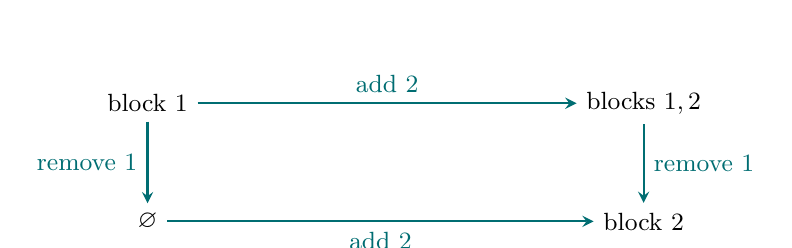
\begin{tikzpicture}[x=1cm,y=1cm,>=stealth,every node/.style={font=\small}]
\node (a) at (0,1.5) {block $1$};
\node (b) at (6.3,1.5) {blocks $1,2$};
\node (c) at (0,0) {$\varnothing$};
\node (d) at (6.3,0) {block $2$};
\draw[->,thick,accent] (a)--node[above]{add $2$}(b);
\draw[->,thick,accent] (b)--node[right]{remove $1$}(d);
\draw[->,thick,accent] (a)--node[left]{remove $1$}(c);
\draw[->,thick,accent] (c)--node[below]{add $2$}(d);
\end{tikzpicture}
\end{center}
The two routes agree up to specified scalars with the finite-level normalizations included. Moving a descent across a longer interval applies one such relation per crossed block. With three blocks, removing the first crosses the second and the third, and subsequently removing the second crosses the third. These are exactly the pairs $(1,2),(1,3),(2,3)$. In general this operation accounts for the index $i<j$ in the scalar $S(\xi)$. The twist on added block $j$ is $\xi^j$. Comparing the characters of blocks $i,j$ therefore involves $\xi^{j-i}$. The associated scalar contains $t$ ratios of partial Hecke values per pair. All first arrows out of an empty interval have ranks $r\to r+t$, so their Gram forms lie in the range of the doubling formula.

The same arrangement proves injectivity. Suppose an entire row of $n+1$ weighted lifts kills the vector coming from the stem. Apply a descent and move it across the row using the square laws. A row of $n$ lifts on the next stem then kills the vector obtained by first lifting and descending. The single-step statement says that lift followed by descent acts injectively between these copies of the stem. Induction starting with the empty chain forces the original vector to be zero. This is how positivity of the full determinant enters before dividing by it.
\route{\sref{Lib/SiegelWeil/RallisInner/Doubling}{doubling and the rank range}, \sref{New/Determinant/Chain/ChainNorms}{intervals and the exchange laws}, \sref{New/Determinant/Chain/TriangleNorms}{induction in the triangle}}

\subsection{How the operators return to the same space}
\label{sec:operator-cancellation}
For fixed $\xi$ let $R_j$ denote the operator of the $j$th Rallis series on the good forms of $Y_0$. These are operators built from translations at unramified places. The single-lift formula initially gives an operator on the good forms of a different rank-$r$ hermitian space $W_j$. The groups at the finite places agree, while their signatures at infinity can differ. A trace comparison for the chosen local types proves that spherical Hecke operators away from the level have the same traces on both spaces. This includes their powers. The trace identities determine the characteristic polynomials, hence the determinants. They also identify the dimensions and the multiplicities of individual simultaneous systems of eigenvalues. This justifies using $R_j$ on the common space in a determinant identity.

The calculation can now be carried out with operators of the correct sizes. Write $d=d_T$, let $u_{\xi}$ be the local factor for the conductor of $\xi$, and put $A_j\ne0$ for the constants of the single-lift formulas. These constants are independent of the twist. The source proves
\begin{align*}
  \Theta_\xi^*\Theta_\xi
    &=c(\xi)u_{\xi}^m\,R_1\cdots R_m,\\
  Z_j(\xi^j)&=(A_j u_{\xi})^d \det R_j .
\end{align*}
All first $m$ powers of the twist have the same conductor support. This is why the same factor $u_{\xi}$ occurs in each row. Taking a determinant in the first identity and substituting the second gives
\[
             Z(\xi)=\left(\frac{c(\xi)}{\prod_{j=1}^m A_j}\right)^d
                       \prod_{j=1}^m Z_j(\xi^j).
\]
For the scalar one takes absolute values and then the ratio with the trivial twist. The fixed constants drop out, and the exchange calculation supplies the magnitude of $c(\xi)/c(1)$. In particular, the scalar is raised to $d$ because it acts on the $d$-dimensional stem. The quantity that multiplies $m$ times is a determinant of an operator on that same stem. This calculation explains why the rank of the much larger last hermitian space never multiplies the main term.
\route{\sref{New/Spanning/Multiplicities/EqualMultiplicities}{trace and determinant comparison}, \sref{New/Determinant/Chain/NormOfChain}{the single-lift and whole-chain identities}}

\subsection{Completing the basis and using the product formula}
Suppose $y_1,\ldots,y_n$ are independent, their untwisted logarithmic squared covolume is bounded by $V_0$ at every conjugate, and their finite-place index is bounded by $\delta$. Complete them by $d_T-n$ auxiliary forms. The proof gives separate bounds for the ordinary sizes of these forms and for the scalars that render their twisted lifts integral. If $n\ge(1-4/b^2)d_T$, their \emph{total} cost is at most $d_T b$. For this completed basis, the untwisted Gram determinant is obtained from the twisted one by multiplication by $Z(1)/Z(\xi_\iota)$. If a matrix $U$ changes the columns, their Gram matrix is transformed to $U^*\operatorname{Gram}U$. Its determinant acquires the two factors $\overline{\det U}$ and $\det U$, explaining the charge $2\delta$ after accounting for conjugate places. The product formula, applied to the common nonzero untwisted determinant, now gives
\[
 0\le V_0+2\delta+d_T b
        +d_T\bigl(b+fa(\log b)^4-H\bigr).
\]
Absorbing the two $b$ terms in the error proves Theorem C,
\[
 \boxed{\quad V_0+2\delta
           \ \ge\ d_T\bigl(H-3fa(\log b)^4\bigr).\quad}
\]
The almost-full dimension matters here. A lone short vector could leave too many expensive directions to complete before applying the product formula.


\route{\sref{New/Determinant/Chain/NormOfChain}{chain factorization}, \sref{New/OneLift/LiftVolumeHeight}{single-lift comparison}, \sref{New/Congruences/FitTwistsExist}{regular twists}, \sref{New/Determinant/Twist/LongForms}{lower bound}}

\subsection{A two-dimensional example of a negative height}
\label{sec:signed-height-model}
Take $V=\mathbb Q^2$ with its standard basis and Euclidean metric after extension to $\mathbb R$. As a model for the untwisted map take $T=\operatorname{diag}(5,1)$. Allow also the identity map. Choose the identity at the prime $5$ and choose $T$ at every other prime. These choices merely illustrate the determinant accounting. In the proof the maps come from arithmetic twists whose existence needs the congruence theorems. For a map $A$ write $Z_A=\det(A^{\mathsf T}A)$. Then $Z_T=25$ and $Z_I=1$.
\begin{center}
\begin{tabular}{@{}lrrr@{}}\toprule
Prime & $Z_{\rm chosen}$ & $Z_T/Z_{\rm chosen}$ & Product\\ \midrule
$5$ & $1$ & $25$ & $25$\\
$\ell\ne5$ & $25$ & $1$ & $25$\\ \bottomrule
\end{tabular}
\end{center}
The first column of numbers forms a family of local units. Its height has upper bound zero with multiplier $1$. For the ratio column choose the single rational multiplier $1/25$. At $5$ the multiplied ratio is $1$. At all other primes it is $1/25$, a unit there. Thus every finite-place charge is zero, while the archimedean charge for the multiplier is $-\log25$. The ratio family therefore has height at most $-\log25$. The last column is a fixed nonzero number. If its archimedean bound is $e^B$, the product formula requires
\[
                          0\le B-\log25 .
\]
Here equality holds. A local choice that gives an especially divisible ratio can enforce a lower bound on an ordinary Euclidean squared volume. In this model all denominators are visible. In the formal proof the index of the original vectors and the cost of completing to a basis are the two additional charges.

\subsection{The product formula with the full list of factors}
\label{sec:local-to-global-volume}
Let $w$ be the family obtained by adjoining $n'=d_T-n$ auxiliary forms to the $n$ given ones, and write $G_\eta=\det\operatorname{Gram}(\Theta_\eta w)$, where $w$ is a basis. At the place $\iota$ use $\eta=\xi_\iota$ and the auxiliary clearing scalar $\gamma_\eta$. There is an exact factorization for every $\iota$,
\[
 G_1=\underbrace{|\gamma_\eta|^{2n'}G_\eta}_{\text{cleared twisted Gram determinant}}\,
      \underbrace{(|\gamma_\eta|^{-2})^{n'}}_{\text{undo the clearing}}\,
      \underbrace{\frac{Z(1)}{Z(\eta)}}_{\text{change the lift}} .
\]
Each factor on the right has a separate height bound. The first costs $2\delta$, the second at most $n'b$, and the third at most $d_T(b+fa(\log b)^4-H)$. The equality holds because $G_\eta=Z(\eta)\det\operatorname{Gram}(w)$. This is the step that needs a full basis. For a proper subspace and a general operator, the squared volume changes by the determinant of its Gram operator restricted as a form to that subspace, a different quantity.

Two conjugations deserve attention. At a finite place the matrix entries of a Gram form are conjugate-linear in one vector. If $\bar\iota(z)=\iota(\bar z)$, one uses a clearing matrix at $\bar\iota$ for that vector and a clearing matrix at $\iota$ for the other. Both matrices work for the \emph{same} twist $\eta$, since the original index bound controls all twists allowed at the underlying prime. The local determinant of the Gram matrix after clearing is integral. Each of the two matrix determinants costs at most the assigned local index, giving $2\delta$ in total.

At infinity a field automorphism $\sigma$ of $\mathbb C$ can change the operation of conjugation on coordinates. For example, the embeddings of a cubic field with one real embedding and two nonreal embeddings already show why an automorphism moving a real algebraic number to a nonreal conjugate requires care. Write $v_i$ for the coordinates of $\Theta_1 w_i$ and $\sigma'=\operatorname{conj}\circ\sigma\circ\operatorname{conj}$. The matrix of the metric is rational. Therefore $\sigma G_1$ is the mixed Gram determinant pairing the vectors $\sigma' v_i$ in the first slot with the vectors $\sigma v_i$ in the second. Cauchy--Schwarz on the exterior power bounds its squared modulus by the product of the two ordinary Gram determinants. This explains the use of the norm bounds on \emph{every} complex conjugate. It gives
\[
                |\sigma G_1|\le \exp(V_0+2n'x_1^2 b^2).
\]
The upper bound here also uses Fischer's determinant inequality for adjoining the new vectors and Hadamard's bound for their individual lengths.

Finally combine this archimedean bound with the three heights above. One formal way to apply the product formula is to multiply the constant family $G_1$ by its inverse, whose height is bounded above by $V_0+2n'x_1^2 b^2$. The resulting family is $1$. Its height bound must be nonnegative. To see the point for a general complex multiplier $H_0$, the proof first shows that a bound on the $2$-adic norm of $H_0$ under \emph{every} identification forces $H_0$ to be algebraic. It applies the rational product formula to the nonzero norm of $H_0$ from $\mathbb Q(H_0)$, and uses the uniform embedding bounds to divide the inequality by the degree. This gives
\[
 0\le V_0+2\delta+n'(2x_1^2b^2+b)
             +d_T\bigl(b+fa(\log b)^4-H\bigr).
\]
The exact bound $n'\le4d_T/b^2$ from Theorem B cancels the $b^2$ in the cost of each added form. Indeed $n'(2x_1^2b^2+b)\le d_T(8x_1^2+4/b)\le d_T b$ by admissibility. The comparison therefore recovers $d_TH$ to the accuracy required by the short-form estimate.
\route{\sref{New/Reduction/Lattices/TwistedLattice}{mixed Gram determinants and the three factors}, \sref{New/Reduction/Lattices/Heights}{product formula for the family $1$}, \sref{New/Determinant/Twist/LongForms}{auxiliary forms and completion costs}}

\section{How one lift recovers the missing main term}\label{sec:one-lift-lab}

The upper calculation has already assigned a logarithmic cost \(H_{\rm dir}\) to an ordinary derivative direction. With \(k\) such directions and \(m\) stages it produces the background \(mkH_{\rm dir}\), in addition to the prime excess one wants to measure. Why should a lower bound based on projections, inner products and special values know this precise coefficient? We follow one stage \(j\). Two identities and a sharpness estimate suffice to locate the coefficient, and each can be understood separately.

\subsection{Changing the metric on the lift space}

Let \(u:S\to T\) be an injective linear map of finite-dimensional complex inner product spaces and put \(L=u(S)\). If \(U\) is an operator on \(T\), let \(C_U=P_L U|_L\) denote its compression to \(L\). In orthonormal coordinates the following identity holds:
\begin{equation}
        \det(u^*u)\,\det C_U=\det(u^*Uu).
        \label{eq:compressionlab}
\end{equation}
To prove it, let \(J:S\to L\) be \(u\) with its range as codomain. Then \(J\) is invertible, and \(u^*\) kills \(L^\perp\). Consequently \(u^*Uu=(u^*u)J^{-1}C_UJ\). Taking determinants gives the formula. It works even when \(U\) carries some vectors of \(L\) outside \(L\). This matters because projection back into \(L\) is precisely where prime denominators can appear.

Here is a two-dimensional example inside a three-dimensional space. Take
\[
 u=\begin{pmatrix}1&0\\1&0\\0&2\end{pmatrix},\qquad
 g=\begin{pmatrix}1&0\\0&0\\0&1\end{pmatrix},\qquad U=gg^* .
\]
The columns of \(u\) are perpendicular, with squared lengths 2 and 4, so their squared area is \(8\). The operator \(U\) deletes the middle coordinate, and \(u^*Uu=\operatorname{diag}(1,4)\). On the lift space \(C_U\) acts by \(1/2\) on \((1,1,0)\) and by 1 on \((0,0,2)\). Indeed \(U(1,1,0)=(1,0,0)\), whose orthogonal projection onto the first direction is \((1/2,1/2,0)\). The two sides of \eqref{eq:compressionlab} both give 4. All of \(u,g,U\) have integral entries. The compression alone has acquired a factor of \(1/2\). An upper bound for the determinant of the compression at the prime 2 needs arithmetic information beyond integrality of \(U\). \sref{New/OneLift/LiftVolumeHeight}{Determinant of a compression and the local eigenvalue bound}.

In the proof \(u=u_\eta\) is the single lift on good forms, with twisting character \(\eta\); \(g_\eta\) glues tuples of test forms on a smaller space into forms on the larger space. The adjoint \(g_\eta^*\) reads a collection of periods of a form. A period is obtained by pairing or integrating a form against specified test data. An exchange calculation proves
\[
            c'_\eta\,g_\eta^*u_\eta=u^\circ ,
\]
with \(c'_\eta\ne0\) and the \emph{same} period map \(u^\circ\) for all twists. This is what makes \(U_\eta=C_0g_\eta g_\eta^*\) an informative choice in \eqref{eq:compressionlab}. The positive factor \(C_0\) is a multiple of stabilizer orders times the square of a hook number from the weight representation. It makes the algebraic construction compatible with integral coordinates. The inner products now satisfy
\[
       u_\eta^*U_\eta u_\eta
           = C_0|c'_\eta|^{-2}(u^\circ)^*u^\circ .
\]
A positive definite form on the fixed source, independent of \(\eta\), has emerged. After taking determinants, the entire dependence on the twist on the right is a scalar to the power \(\dim S=d_T\).

Write \(P_j(\eta)\) for the product of Hecke special values with its local normalizations and put \(\rho_\eta=P_j(\eta)/P_j(1)\). The exchange formula identifies this scalar ratio with \(|c'_1|^2/|c'_\eta|^2\). If \(Z_j(\eta)=\det(u_\eta^*u_\eta)\) and \(\Delta_\eta=\det C_{U_\eta}\), division of the twisted and untwisted identities gives
\begin{equation}
       \frac{Z_j(1)}{Z_j(\eta)}
         =\frac{\Delta_\eta}{\Delta_1}\,\rho_\eta^{-d_T}.
       \label{eq:delta-rho}
\end{equation}
The determinant of the common positive definite form is nonzero. This justifies cancellation even for the individual twists chosen later at finite places. \sref{New/OneLift/LiftVolumeHeight}{Gluing adjoint, positive comparison form and volume ratio}.

\subsection{What it takes to use this identity at a finite prime}

The map \(g_\eta g_\eta^*\) has another advantage. Writing the identity on the tuple space as a sum of rank-one operators from a tight frame writes \(U_\eta\) as a sum of rank-one operators on integral test forms, with known normalization. It preserves integrality away from the conductor. On a genuine lift its output is orthogonal to the false lifts. These are forms in the orthogonal complement of the genuine lifts that satisfy the selected local type and an annihilating Hecke-polynomial condition at the split place in question. The latter condition can hold for more forms than come from the intended lift. The orthogonality result lets the proof apply the arithmetic projection bound on the particular vectors it needs.

There is a useful distinction between clearing every coordinate by one large scalar and estimating the determinant of an operator that clears the projection on this subspace. In the latter formulation let \(B_\ell\) be such a clearing operator on the genuine lifts. If its determinant has \(\ell\)-adic norm at least \(\exp(-d_T r\beta_\ell)\), then
\[
              |\Delta_\eta|_\ell\le \exp(d_T r\beta_\ell).
\]
Indeed \(B_\ell C_{U_\eta}\) takes integral lifts into integral lifts. Its eigenvalues have norm at most 1. One way to see this in lattice coordinates is to scale an eigenvector until its largest coordinate has norm 1. An integral operator takes it to a vector of norm at most 1, bounding the norm of its eigenvalue. Multiplying the eigenvalues gives \(|\det(B_\ell C_{U_\eta})|_\ell\le1\); dividing by the lower bound for \(|\det B_\ell|_\ell\) gives the claim. The formal proof uses the integral gauge on forms for the normalization of the eigenvector. Its hypotheses allow different clearing operators at different primes.

At infinity the proof controls every conjugate of \(\Delta_1\) from above by \(\exp(3d_T f m b(\log b)^2)\). Thus \(\Delta_1\ne0\) can be the fixed multiplier in the height of the family \(\Delta_{\xi_\iota^j}/\Delta_1\). The archimedean contribution is paid once per stage, and the finite-place charges are bounded by summing the projection allowances. This first factor of \eqref{eq:delta-rho} has accounted for a cost. The negative main term is in the second factor. \sref{New/OneLift/LiftVolumeHeight}{Tight frame, integral comparison operator and both determinant bounds}.

\subsection{Why divisibility also has to be sharp}

Theorem A gives derivatives divisible \emph{at least} to a predicted order. Such a statement allows every test coefficient to vanish. In the lower bound one needs a test form whose pairing with a rank-one lift has valuation \emph{at most} a predicted order plus a controlled loss. A large guaranteed common divisor and a witness close to that common divisor play different roles, just as divisibility of a list of integers by \(p^h\) leaves open whether all of them are divisible by \(p^{h+1}\).

There is an elegant argument for finding a witness on a single CM curve. Let \(y\) be its local parameter in the specified normalization, \(\mathcal O\) the \(p\)-adic valuation ring, and use the valuation \(v_p(p)=1\). Define \(M_n\) to be the greatest \(p\)-adic norm of \(f^{(n)}(0)\) among \(f\in\mathcal O[[y]]\), with derivatives in the additive uniformizing coordinate. Each fixed coefficient depends on only finitely many powers of \(y\). The nonarchimedean triangle inequality shows the maximum is attained by a power of \(y\). In these coordinates \(0\le M_n\le1\), \(M_0=1\). The integral formal group law writes \(y(z+w)\) as an integral series in \(y(z)\) and \(y(w)\). Differentiating \(n\) times in \(z\) and \(h\) times in \(w\) consequently gives
\[
                              M_{n+h}\le M_n M_h .
\]
A bound in this direction says that a loss at even one order propagates under repeated addition.

Set \(q_p\) equal to the residue-field size and \(e_p\) to the ramification index of the quadratic field at \(p\). The scaled formal parameter has a unit coefficient after rescaling in degrees \(N=q_p^a\). Removing the scale gives a coefficient of valuation \(-(N-1)/(e_p(q_p-1))\). Converting it into a derivative multiplies by \(N!\), of valuation \((N-1)/(p-1)\), since \(N\) is a power of \(p\). The resulting rate is
\[
            \gamma_p=\frac{1}{p-1}-\frac{1}{e_p(q_p-1)} .
\]
In particular \(M_N\ge p^{-(N-1)\gamma_p}\) in arbitrarily large degrees. Write \(c=p^{-\gamma_p}\le1\). If \(M_n<c^n\) at any fixed \(n>0\), divide these large \(N\)'s as \(N=un+r\), \(0\le r<n\). Then
\[
        \frac{M_N}{c^N}\le
        \left(\frac{M_n}{c^n}\right)^u\frac{M_r}{c^r}\longrightarrow0 ,
\]
contradicting \(M_N\ge c^N\). Thus \emph{in every degree} some derivative has valuation at most \(n\gamma_p\). This passage from rare explicit coefficients to all required orders is one of the smaller insights hidden inside the lower bound. For an inert prime the answer simplifies to \(p/(p^2-1)=p^{-1}+p^{-3}+\cdots\), exactly the odd-power rate in the local divisibility calculation. \sref{New/Derivatives/Sharpness/OneCurve}{Sharpness on the curve and submultiplicativity}.

The bridge to the actual critical values is substantial. The coefficients lie on a CM field with several places and prescribed nearby degrees \(\kappa_\tau\le l_\tau\le\kappa_\tau+x^{42}\). Partner places can interfere. The readable proof uses products in disjoint copies of variables, bounds the losses from close pairs of places, and transfers a coefficient to theta data supported on one residue class. With twelve copies it produces a \emph{single} nonzero number \(t_0\) of controlled complex size. For every \(p\) it supplies an indicator datum and a Taylor coefficient \(a_{\gamma,p}\) of the prescribed degrees for which
\[
   v_p\!\left(c_{\rm vac}^{12}\Bigl(\prod_\tau l_\tau!\Bigr)a_{\gamma,p}\right)
                   \ \le\ S_p+v_p(t_0),
   \qquad |\sigma(t_0)|\le \exp(fmb/k).
\]
Here \(c_{\rm vac}\) normalizes the vacuum, \(S_p\) is the ordinary-direction gain at \(p\) summed over places, and the valuation refers to the chosen embedding. The datum and coefficient may vary with \(p\). A witness in one degree on one curve supplies an ingredient; the multivariable statement, the placement in a rank-one lift, and orthogonality of the resulting test form each require their own arguments. \sref{New/Derivatives/Sharpness/BoundAttained}{Coefficient at every prime}; \sref{New/OneLift/HeckeValues/TwistedValueHeights}{test-form pairing and the ratio of critical values}.

\subsection{The coefficient on both sides, counted exactly}

One can now read the claimed main term off an exact factor count. For the \(j\)-th lift the product ratio \(\rho_\eta\) has the form
\[
 \rho_\eta=(\mathrm{N}\mathfrak q_\eta)^e
  \left(\prod_{a\in A_j} r_a(\eta)
          \prod_{c\in B_j} r_c(\eta^{s_c})\right)^2 ,
       \qquad 2|A_j|=k,\quad |B_j|=5m .
\]
The \(r\)'s are ratios of absolute values of partial Hecke \(L\)-functions at specified integers, \(s_c=\pm1\), and the indexing sets are independent of the twist. The symbols \(A_j,B_j\) here enumerate special values, distinct from the earlier sets of infinite places. The norm of the conductor is a unit at the chosen finite prime. Put \(D_{\rm den}=fa(\log b)^3/(mk)\). The inverse ratio of each main pair in \(A_j\) has height bounded by \(6D_{\rm den}-H_{\rm dir}\). Its sign comes from the test pairing and the comparison of its finite valuation with its archimedean normalization. The remaining \(5m\) inverse ratios each cost at most \(x_1\). Taking the product, including its square, gives exactly
\[
       h(\rho^{-1})\ \le\
         \underbrace{k(6D_{\rm den}-H_{\rm dir})}_{2(k/2)\ \mathrm{main\ factors}}
            +\underbrace{10mx_1}_{2(5m)\ \mathrm{other\ factors}} .
\]
The \(\rho^{-d_T}\) in \eqref{eq:delta-rho} multiplies these terms by \(d_T\). The other errors, including the cost of \(\Delta_\eta/\Delta_1\), fit inside \(d_T k(\log b)D_{\rm den}\) once combined with the positive terms above. Each stage thereby contributes a main term \(-d_T kH_{\rm dir}\) in its height estimate. After \(m\) stages one obtains \(-d_TmkH_{\rm dir}\). Application of the product formula transfers it to the other side of the inequality as \(+d_T H\).

The upper proof counted \(k\) ordinary directions per step. The lower proof counted \(k/2\) distinguished values in a \emph{squared} product. Missing that square would return only half of \(H\). As Section~\ref{sec:compare} quantifies, even a small fixed fractional error in \(H\) would exceed the permitted error by a growing power of \(x\). The coefficient identity explains why the proof calculates such specialized periods when its ultimate goal is an estimate for primes. \sref{New/OneLift/HeckeValues/TwistedValueHeights}{The factor count and inverse-ratio bound}; \sref{New/OneLift/LiftVolumeHeight}{height of one lift}.


\section{Why a congruence between forms affects their volume}\label{sec:galoisbridge}
The lower bound has to estimate how far an integral test form can move outside an integral lattice when it is projected onto the space of genuine lifts. This is where Galois representations and Selmer groups enter the proof about prime sums.

\subsection{A denominator visible in an eigenvalue difference}
Return to projection onto the line through \((1,2)\), and introduce the integral symmetric matrix
\[
      T=\begin{pmatrix}1&2\\2&4\end{pmatrix}.
\]
It has eigenvalue \(5\) on that line and \(0\) on the line through \((-2,1)\). Over \(\mathbb Q\) its spectral projection onto the first line is \(P=T/5\). In particular \(P(1,0)=(1,2)/5\). At the prime \(5\) the two eigenvalues coincide modulo the maximal ideal. Indeed, the reductions of the two eigenlines coincide there as well. This example exhibits a simple relationship: separating two systems of eigenvalues over a field can introduce the prime divisors of their difference into the denominators of a projector.

In the automorphic setting there are many commuting Hecke operators, and many eigensystems may remain congruent at once. The proof constructs an endomorphism \(\Lambda\) of the lift space \(Z\). For the allowed integral test forms \(v\), the vector \(\Lambda\,\mathrm{pr}_Z v\) is integral at the chosen \(\ell\)-adic identification. The tests satisfy an orthogonality condition on the false lifts described above. The quantitative assertion includes
\[
       \bigl|\det\Lambda\bigr|_\ell
          \ \geq\ \exp\{-\dim(Z)\,r\,\beta_\ell\},
\]
where \(r\) here is the rank of the source hermitian space for the lift in question. In the two-dimensional example multiplying by \(5\) clears the projection denominator. In the general case the eigenvalues of the clearing operator can have different valuations. A determinant bound suffices because the eventual comparison is a volume calculation.

\subsection{From Hecke eigenvalues to extension classes}
A Hecke eigensystem is the list of eigenvalues by which commuting arithmetic operators act on a form. The proof transfers suitable information in these lists to representations of the absolute Galois group of the CM field. For a genuine lift the traces of a normalized representation have a recognizable shape: a main summand, twisted by a character, together with a specified string of powers of the inverse cyclotomic character. The cyclotomic character records Galois action on roots of unity. The fact that the main block can be used across different twists lets one control a fixed finite family. This assertion is established for the local types and ranks of the construction. See the \sref{New/Congruences/GaloisRepresentations/RowsFromEigensystems}{main-summand theorem}.

A two-dimensional calculation explains the appearance of cohomology. Suppose a group acts on a module preserving a line. In a basis beginning with that line the matrices have the shape
\[
 \rho(g)=\begin{pmatrix}\alpha(g)&b(g)\\0&\nu(g)\end{pmatrix}.
\]
Assume \(\alpha,\nu\) are characters, with \(\nu(g)\) invertible. Multiplying the matrices for \(g,h\) gives, for \(z(g)=b(g)/\nu(g)\),
\[
 z(gh)=z(g)+(\alpha/\nu)(g)\,z(h).
\]
This is the cocycle equation for the action through \(\alpha/\nu\). Replacing the second basis vector by itself plus \(c\) times the first changes \(z(g)\) by \(((\alpha/\nu)(g)-1)c\). Such changes are coboundaries. Thus a cohomology class records whether the extension can be made diagonal by a change of splitting. The trace \(\alpha(g)+\nu(g)\) alone has forgotten that class. Integral lattices and reduction modulo powers of \(\ell\) are where the extra information relevant to congruences is recovered.

A Selmer group is a group of cohomology classes satisfying specified conditions on restriction to the local Galois groups. Its length over a local coefficient ring counts the successive layers of divisibility. For example, \(\mathbb Z_\ell/\ell^h\mathbb Z_\ell\) has length \(h\). In the proof lengths are normalized so that the quotient by \(\ell\) has length one after extensions of the coefficient ring. A uniform estimate for the relevant lengths limits how much congruence can persist in the Hecke projector. The formal version of this implication is substantially stronger than the two-dimensional example. A first-order form of Ribet's method constructs an element controlling determinants of several matrix relations at once. The denominator theorem converts this element and estimates for local errors into the operator \(\Lambda\) above. The exact interfaces are \sref{New/Congruences/FirstOrder/RibetLemma}{the common Ribet element} and \sref{New/Congruences/FirstOrder/DenominatorBound}{the clearing bound}.

\subsection{Making one twist serve several powers}
At a fixed rational prime \(\ell\), choose an identification of coefficients \(\iota\) with an algebraic closure of \(\mathbb Q_\ell\). Several constraints must hold at once. The determinant formula uses \(\xi_\iota,\xi_\iota^2,\ldots,\xi_\iota^m\). The main summands arise from both rank-\(r\) eigensystems and the rank-one lifts used to evaluate Hecke values. Finally, the inverse of each required twisted special-value ratio must have controlled \(\ell\)-adic size. Choosing the best twist separately for each factor would leave no guarantee about the determinant of a \emph{single} twisted chain.

The construction adds auxiliary split places away from \(\ell\) and the old level. Their Frobenius and tame inertia elements can be selected with prescribed properties by a Chebotarev argument. At such a place a linear condition of the form
\[
         z(\text{tame generator})
                 =s_v\,z(\text{Frobenius})
\]
ties two values of a cocycle. A duality count for these local conditions compares the length of a constrained Selmer group with a dual group and explicit local errors. The construction packages the resulting constraints on the twist into finitely many polynomials. It also packages conditions on special values by means of elements of class-group rings with norm relations. Evaluating at carefully chosen roots of unity then selects an anticyclotomic character that works simultaneously for the finite list and for every needed power. Small Selmer groups here means bounded length; the argument allows a residual cost. The finite list can be large, since its size is determined \emph{after} the data for \(x\) have been chosen.

For each \(\iota\) the output is a character whose conductor avoids \(\ell\), bounds for projection denominators, and bounds for inverse ratios of the designated special values. The resulting family can vary with \(\iota\); the untwisted Gram determinant to which the product formula is applied is fixed. The \sref{New/Congruences/Selmer/AuxiliaryPrimes}{choice of auxiliary places}, \sref{New/Congruences/Selmer/Count}{duality count}, \sref{New/Congruences/Selmer/GeneralTheorem}{simultaneous specialization} and \sref{New/Congruences/FitTwistsExist}{regular-family theorem} give successive entry points.

\subsection{Where the square of the chain length occurs}
There is a way to see why a square-root-length chain is compatible with the cost of these denominators. The sum allowed for denominators per lift and source direction is
\[
            B_{\mathrm{den}}=\frac{fa(\log b)^3}{mk}.
\]
One contribution to the estimate for clearing all primes is the local defect. The proof bounds its total, weighted by \(\log\ell\), on any finite set of primes by
\[
       C f\frac{m}{k}\,b\log b,
             \qquad C=4\cdot10^6 e^{180}.
\]
This displayed quantity is an \emph{upper bound} for one contribution. Divide it by the available budget and substitute \(a=xb\). The ratio simplifies to
\[
       C\frac{m^2}{x(\log b)^2}.
\]
With \(\sqrt x\le m\le2\sqrt x\) it is at most \(4C/(\log b)^2\). As \(x\) grows the prescribed scales make this arbitrarily small. The criterion at the end of the proof rewards the length \(m\) because the prime discrepancy is multiplied by \(m\). The denominator accounting here charges for \(m\) twice, once in the local loss and once when allocating the budget. If one tried the formal substitution \(m=x^{1/2+\delta}\), the same ratio would have a numerator \(x^{2\delta}\). It could no longer be absorbed for arbitrarily small choices of the exponent controlling \(\log b\) by this calculation alone. This calculation explains the square-root choice within the estimates proved here. Other constructions would require their own analysis of the denominator cost.

The bound on the total clearing cost includes further terms. Some are bounded by fixed powers of \(x\) with large exponents, such as \(x^{4000}\). They are harmless here because \(b\) grows faster than any fixed power of \(x\) when the small positive scale exponent is fixed. The distinguishing feature of the local-defect term is that it too contains \(b\); comparison requires the finer cancellation of scales just displayed. The estimates and their final sum appear together in the \sref{New/Congruences/FitTwistsExist}{source for regular twists}.

\section{Which part of a congruence costs volume?}\label{sec:denominatorlab}

Projecting an integral form onto an eigenspace can put a large prime power in its denominator. The small matrix in Section~\ref{sec:galoisbridge} made this visible for two eigenvalues. Suppose now that ten thousand systems of Hecke eigenvalues nearly agree with the one we want. Multiplying ten thousand differences of eigenvalues would separate it from its competitors over a field, provided each difference was chosen to detect the corresponding competitor. The valuation of that product could ruin the lower bound. The actual argument can afford enormous divisibility in an \emph{intermediate} separator. The valuation eventually charged to the determinant comes from a different coefficient. We trace the changeover at one prime.

Fix a coefficient identification at $\ell$ and one of the single lifts. Write $Z$ for its space of genuine lifts, $P$ for orthogonal projection onto $Z$, and $N_x(g)$ for the normalized Galois matrix of an eigensystem $x$ at a group element $g$. An input form $v$ is integral and orthogonal to the false lifts in the specified types. The problem is to find a linear operator on $Z$ which makes $Pv$ integral, and whose determinant has bounded valuation.

\subsection{What a root of the Hecke polynomial can detect}

Set $\delta_g(x)=\det(1-N_x(g))$. At a genuine lift the normalized eigenvalue data include the zeroth power of the cyclotomic character, namely the trivial character. Thus $\delta_g(x)=0$ for every $g$. The source calls a system satisfying the latter condition a \emph{weak lift}. The distinction between a common fixed vector and a fixed vector for each $g$ is worth seeing in an example.

Let the Klein four group act on three coordinates in characteristic zero, with generators
\[
  a=\operatorname{diag}(1,-1,-1),\qquad
  b=\operatorname{diag}(-1,1,-1).
\]
The fixed lines of $a$, $b$ and $ab$ are the first, second and third coordinate axes respectively. Each group element has eigenvalue $1$. The intersection of the fixed spaces is zero. In fact $a+b+ab=-I$, so the sum of the three matrices $1-a$, $1-b$, $1-ab$ is $4I$, with nonzero determinant. This finite group illustrates a gap in the proposed inference. A proof using only the individual equalities $\delta_g(x)=0$ would need another argument to recognize the image of the lift.

The extra information is orthogonality. At a suitable split place the local Hecke polynomial, acting at the distinguished lift root, kills the weak systems at base level. Identification of that root uses a local theorem giving a whole chain of roots, with successive ratio the residue-field order. After projection to a type, any weak component in $Z^\perp$ of the specified kind lies among the false lifts. The test form has zero pairing with these components. In the form used in Lean, if a subspace $M$ contains every relevant isotypic vector in a non-weak system, and the stated stability and type conditions hold, then
\[
                P_{\rm type}(v-Pv)\in M .
\]
Taking $M$ to be a suitable kernel lets a diagonal operator act on the integral $v$ in place of its possibly nonintegral projection. The period comparison constructs inputs $v=Uz$ orthogonal to the false lifts, so the proof can invoke this result for precisely the vectors it needs.
\route{\sref{New/Congruences/FirstOrder/DenominatorBound}{weak systems and the type component of the error}, \sref{New/Congruences/FirstOrder/HeckeStrings}{the chain of Hecke roots}, \sref{New/OneLift/LiftVolumeHeight}{orthogonality of the comparison operator}}

\subsection{A separator with an uncontrolled valuation}

For every non-weak system $y$ at base level choose a single $g_y$ with $a_y=\delta_{g_y}(y)\ne 0$. These numbers are integral at $\ell$ because the characteristic polynomials have integral coefficients. Write $\mathcal Y$ for this finite set of non-weak systems and form the simultaneous separator
\[
        D(x)=\prod_{y\in\mathcal Y}(a_y-\delta_{g_y}(x)),\qquad
        n_0=\prod_{y\in\mathcal Y}a_y .
\]
At a non-weak $x$, its own factor vanishes. At a weak $x$, $D(x)=n_0\ne0$. Consequently $D/n_0$ is exactly the indicator of the weak systems at this level. Its expression has introduced a denominator for which all we know so far is nonvanishing. Even a product of numbers with quite modest valuations can be expensive when there are many factors.

Two ingredients recover control. First, a Hecke-algebra polynomial $F$ turns every $\delta_g$ into an element of a particular ideal $\mathfrak a$ upon multiplication. Traces expressing local relations on the representations and finite-precision terms generate this ideal. The elementary algebraic consequence is
\begin{equation}
                      (D-n_0)F\in\mathfrak a .                 \label{eq:denom-ribet}
\end{equation}
Indeed, expanding $D-n_0$ leaves only terms containing at least one $\delta_{g_y}$. This is why the \emph{same} $F$ must serve all $g$. Second, one can make the precision of the local construction as deep as the valuation of $n_0$ requires. To see what survives after using that precision, we need the coefficient of $F$ supplied by the arithmetic.
\route{\sref{New/Congruences/FirstOrder/DenominatorBound}{the product over non-weak systems}, \sref{New/Congruences/FirstOrder/AuxiliaryPrimeTie}{the product difference and the tied ideal}}

\subsection{Why take the coefficient of every auxiliary variable once?}

At a finite ordered set of auxiliary places $J$ introduce variables $X_j$. A model relation in the group algebra is
\[
     (\tau_j-1)-X_j(\phi_j-1)H_j(\phi_j),
              \qquad H_j(1)=1.
\]
Here $\tau_j$ is tame inertia and $\phi_j$ is Frobenius. The Hecke algebra sees traces of products of this relation with group elements. The variables record how inertia is tied to Frobenius, with conjugate places treated together. These variables belong to the first-order congruence argument. The character-selection polynomials in Section~\ref{sec:bridgelab} serve a separate purpose.

The common Ribet element $F$ has two properties beyond \eqref{eq:denom-ribet}. At every designated lift system all its coefficients of \emph{proper squarefree divisors} of $X_J=\prod_{j\in J}X_j$ vanish. At a specified lift system $x_0$, its coefficient $d_0=[X_J]F(x_0)$ has a quantitative valuation bound. Squarefree means that each variable has exponent zero or one. A term $X_1^2$ is allowed in $F$. Its exponent makes it irrelevant to the coefficient we will extract. For two places the observation amounts to calculating in $\mathcal O[X_1,X_2]/(X_1^2,X_2^2)$, with $\mathcal O$ a local coefficient ring. The surviving polynomial at $x_0$ is simply $d_0X_1X_2$. This explains the phrase \emph{first order}. One keeps at most the first power in \emph{each} local variable, however many places are involved.

Where does the bound for $d_0$ come from? Relations among the matrices $N_x(g)-1$ impose relations on cocycles. Over a discrete valuation ring $\mathcal O$, the maximal minors of a matrix presenting a finite quotient measure its length. For instance, with uniformizer $\pi$, the relation rows $(\pi^a,1)$ and $(0,\pi^b)$ present a quotient of length $a+b$. Their determinant has exactly this valuation, even though one relation mixes the two coordinates. The proof needs this principle over the polynomial ring $\mathcal O[X_j]$. It uses the ideal generated by full-size determinants of relation rows, the zeroth Fitting ideal. One result is that for a set of indices $I$ belonging to one character block the ideal contains
\[
             \left(\prod_{j\in I}X_j\right)B(X),\qquad
             v_\pi(B(0))\le b_0+(|I|+|S|)v_\pi(C).
\]
Here $S$ indexes a finite set of tests, $C$ is a scalar covering a separation loss, and $b_0$ bounds the lengths in the lemma's triangular hypotheses. Successively imposing one local relation isolates one variable per place. Determinant relations for the main summand and the character blocks are then combined. The length charged for the main summand is bounded using its Selmer group. For even character cocycles the ordered places ensure that vanishing at earlier tests controls the next one up to the prescribed loss. This triangular property of carefully chosen primes allows the estimate to dispense with a bound for the total size of all those even class groups.

In the Galois application write $c$ for the fixed group-order multiple that clears stabilizers, $r'$ for the source rank, $t'$ for the rank difference, $s$ for the Selmer-length bound and $h$ for the ramification allowance. In the normalization $v_\ell(\ell)=1$ the theorem obtains
\begin{equation}
       v_\ell(d_0)+2v_\ell(c)
       \ \le\ s+2t'h+r'\,\mathrm{loc}_\ell+e_\ell .            \label{eq:denom-coeff}
\end{equation}
The last two terms represent the local defect contribution and the explicit remaining error. The factors $a_y$ have disappeared from the right-hand side. Construction of $F$ uses the hypotheses on local types, Galois representations, lattices and auxiliary places. The elementary determinantal calculation illustrates how length enters the estimate.
\route{\sref{New/Congruences/FirstOrder/FittingBlock}{triangular Fitting ideals and the common element}, \sref{New/Congruences/FirstOrder/RibetLemma}{assembling the blocks}, \sref{New/Congruences/FirstOrder/RibetElement}{the valuation of the squarefree coefficient}, \sref{New/Congruences/FirstOrder/EvenClasses}{the conditions on the ordered primes}}

\subsection{How extra precision pays for an arbitrarily large separator}

Each auxiliary place also supplies an integral operator $\partial_j$. It deforms the ordinary finite-group sum $\mathrm{Nm}_j$ in that local direction. The source multiplies the factors $\mathrm{Nm}_j+X_j\partial_j$ and uses their coefficients as operators. The resulting family $\mathcal N$ annihilates the tied ideal after the prescribed reduction, when read at the coefficient $X_J$. It also factors through the base-level norm after insertion of specified powers of an integral Hecke operator. These two properties connect the polynomial identity \eqref{eq:denom-ribet} with integrality of forms at base level.

There is a direct way to see why the top coefficient is correctly placed. Write $F_U=[\prod_{j\in U}X_j]F$. In two variables the product has coefficient
\[
 [X_1X_2](\mathcal NF)
   =\mathcal N_{\varnothing}F_{12}
    +\mathcal N_1F_2+\mathcal N_2F_1+\mathcal N_{12}F_{\varnothing}.
\]
On a vector supported on the lifts, $F_{\varnothing},F_1,F_2$ vanish. The only term to survive there is the ordinary norm $\mathcal N_{\varnothing}$ applied to the desired coefficient. In general the terms are indexed by complementary subsets of $J$, and the same reasoning singles out $F_J$. Simultaneously, \eqref{eq:denom-ribet} licenses replacing $D$ by $n_0$ in the appropriate reduced calculation. The cutoff to the systems congruent to $x_0$ is an integral idempotent $A$. In this calculation its power $A^{|J|+1}$ acts in the same way as $A$.

Here is the precision requirement that makes cancellation legal. Write $n$ for the rank of the larger hermitian space and choose the auxiliary level so that, in the valuation ring,
\[
             2n!\,(n_0c^2)^{|J|+1}\ \mid\ \ell^\nu .
\]
The order of choices matters. The finite product $n_0$ is nonzero, and the auxiliary-prime theorem fixes the finite ordered index type $J$ before asking for precision $\nu$. One can therefore choose $\nu$ this large and still obtain the required primes. The lower-bound estimate incurs no charge proportional to $\nu$. The elementary cancellation behind this step is worth spelling out. In a lattice $L$ over the valuation ring, if $a\ne0$, $a\mid b$, and $az=au+bw$ with $u,w\in L$, then $z=u+(b/a)w\in L$. Sufficient precision is what makes $b/a$ integral.

The source performs the operator calculation with $a=(n_0c^2)^{|J|+1}$ after allowing for $2n!$. The coefficient it delivers, up to fixed normalization and $A$, is $F_J$. Thus the price of distinguishing the systems need only be paid in the depth of the auxiliary calculation. The valuation charged to the final operator is bounded by \eqref{eq:denom-coeff}. Treating $D/n_0$ as the final projector would conceal this distinction.
\route{\sref{New/Congruences/FirstOrder/AuxiliaryPrimeTie}{the deformed norm, its factorization and cancellation at the top coefficient}, \sref{New/Congruences/FirstOrder/DenominatorBound}{choice of the level after the index type}}

\subsection{Choosing a single operator on the lift space}

At this point each lift generator can be handled separately. Choose a basis $z_1,\ldots,z_d$ of $Z$ among the generators. For its $i$-th member the construction gives an operator $G_i$ on $Z$, diagonal in that basis. It takes $Pv$ to an integral vector for every allowed $v$, and its eigenvalue on $z_i$ has valuation at most the explicit bound. The argument has given no comparable lower bound on the norms of its other eigenvalues. Multiplying the operators could therefore give a singular operator.

Consider a two-operator model at $\ell=2$ on three directions. Take
\[
       G=\operatorname{diag}(1,0,1),\qquad
       H=\operatorname{diag}(0,1,1).
\]
Every direction has a unit eigenvalue on at least one of the two operators. Yet every combination $uG+vH$ with $u,v\in\mathbb Z_2$ has a non-unit eigenvalue. Its eigenvalues are $u,v,u+v$. If the first two are units, the third is even. Over the valuation ring of $\overline{\mathbb Q}_2$ take $u=1$ and $v=\omega$, a primitive cube root of unity. All three are units, since $1+\omega=-\omega^2$, and the determinant is $-1$. The extension of the residue field has made simultaneous success possible.

In general write $g_{ik}$ for the eigenvalue of $G_i$ on $z_k$, viewed $\ell$-adically. Choose in each column a nonzero entry $m_k$ of largest norm. The linear polynomial $\sum_i(g_{ik}/m_k)U_i$ now has integral coefficients, one of them a unit. Its reduction is nonzero. The residue field $\overline{\mathbb F}_\ell$ is infinite, so one tuple avoids the finitely many hyperplanes where one of these linear forms vanishes. One proof takes their product. A nonzero polynomial over an infinite field cannot vanish on the entire affine space. Lift the coordinates of a good tuple to integral $u_i$. Then
\[
   \left|\sum_i u_i g_{ik}\right|_\ell
          =|m_k|_\ell=\max_i|g_{ik}|_\ell
          \qquad\text{for every }k .
\]
The sum $\sum_i u_iG_i$, with coefficients carried back through the fixed identification, is still a clearing operator, because integral vectors are closed under integral linear combinations. It simultaneously attains at least the norm available to each direction separately. Multiplication by the fixed stabilizer multiple $c$ also gives integral pairings with every test vector integral at all places above $\ell$. For the resulting operator $\Lambda$ the determinant bound is
\[
              |\det\Lambda|_\ell
                    \ \ge\ \ell^{-d r'\beta_\ell},
\]
where $\beta_\ell$ is the local clearing bound before multiplication by $\log\ell$. This is what the volume comparison requires. The large number of unwanted systems first affected an auxiliary precision. The number of basis directions now enters as the dimension $d$ in a determinant, just as it does in the volume on the other side of the proof.
\route{\sref{New/Congruences/FirstOrder/HeckeStrings}{combining diagonal operators}, \sref{New/Congruences/FirstOrder/DenominatorBound}{one generator, the full lift space and the final pairing bound}}

\section{How one character survives every test in the chain}\label{sec:bridgelab}

At a finite place one needs a character $\xi$ for which all $m$ lifts fit together. Its powers enter both the Gram determinant and the projection denominators. A choice of $\xi$ that makes the first projection nearly integral can make a later special value highly divisible. Choosing a different character for the later lift breaks the comparison with the determinant of the chain. There is a way to solve all these requirements at once by counting how often a polynomial can be small on the roots of unity. The proof of this fact involves an elementary harmonic sum. We follow it because it explains how conditions of two apparently different kinds can share one character.

\subsection{Two polynomials that reject a proposed character}

Consider an example over the algebraic closure of $\mathbb Q_3$. Write $v$ for the $3$-adic valuation, with $v(3)=1$ and $v(0)=+\infty$. A positive valuation means divisibility. A large valuation at a selected point will be expensive. Let
\[
    P_1(X)=\Phi_3(1+X),\qquad P_2(X)=\Phi_9(1+X),
\]
where $\Phi_n$ is the cyclotomic polynomial. Both take the value $3$ at $X=0$. We want the values of both polynomials at $X=\zeta^j-1$ to have bounded valuation for $1\le j\le3$. If $\zeta$ has order $9$, then $P_2(\zeta-1)=0$. Increasing its order to $27$ fixes this first test, but $\zeta^3$ has order $9$, so $P_2(\zeta^3-1)=0$. Taking a power can move an otherwise good choice directly onto an exceptional point.

Take $\zeta$ of order $81$. If $\eta$ has order $3^h$ and $k<h$, the quotient formula for $\Phi_{3^k}$ gives
\[
 v(\Phi_{3^k}(\eta))
 =v(\eta^{3^k}-1)-v(\eta^{3^{k-1}}-1)=3^{-(h-k)}.
\]
Indeed a primitive root $u$ of order $3^a$ has $v(u-1)=1/(2\cdot3^{a-1})$. The two terms of the difference therefore have ratio $3$. All six tests are now explicit.

\begin{center}
\begin{tabular}{@{}rrrr@{}}\toprule
Power $j$ & Order of $\zeta^j$ & $v(P_1(\zeta^j-1))$ & $v(P_2(\zeta^j-1))$\\ \midrule
1 & 81 & $1/27$ & $1/9$\\
2 & 81 & $1/27$ & $1/9$\\
3 & 27 & $1/9$ & $1/3$\\ \bottomrule
\end{tabular}
\end{center}
This example has rational coefficients and two prescribed exceptional orders. In the proof the coefficients can be arbitrarily ramified algebraic integers over $\mathbb Q_\ell$. The polynomials can have many variables, and even their degrees can depend on the supply of available characters. A degree bound for avoiding finitely many roots would give the choices in the wrong order. We need an upper bound on the orders of the roots of unity before we know which polynomials will arise.

\subsection{Turning arithmetic conditions into polynomial evaluations}

Fix the data for $x$, a rational prime $\ell$, and an identification of the algebraic coefficients with $\ell$-adic ones as in the proof. Here $Q$ denotes the finite set of auxiliary places of the CM field $E$ used by the twist construction. The progression modulus resumes its earlier meaning in the next section. With each $u\in Q$ it constructs a homomorphism $\lambda_u$ from the absolute Galois group of $E$ to $\mathbb Z/\ell^N\mathbb Z$. At inertia above $u$ this homomorphism takes the value $1$. The other $\lambda$'s vanish there. Each $\lambda_u$ is anticyclotomic, meaning that conjugation by complex conjugation negates its value in the additive cyclic group. Given roots of unity $\zeta_u$ of orders dividing $\ell^N$, set
\[
       \psi(g)=\prod_{u\in Q}\zeta_u^{\lambda_u(g)},\qquad
       X_u=\zeta_u-1 .
\]
Changing any representative of $\lambda_u(g)$ by $\ell^N$ leaves this expression unchanged. It defines a character, is trivial on decomposition groups above $\ell$, and inverts under complex conjugation. On inertia at $u$ it takes the value $\zeta_u$ on some element. Thus if $\zeta_u^j\ne1$ for all $u$ and $j\le m$, each positive power under consideration ramifies at every place of $Q$.

There are two sorts of polynomial. For a group-ring element $\Theta_Q=\sum_g c_g[g]$ on the relevant finite class group, evaluation sends $[g]$ to the value of the character at $g$. A monomial in the $1+X_u$ expresses this value, using the chosen representatives of the finite cyclic exponents. Summation gives a polynomial that evaluates to $\psi(\Theta_Q)$ at every permitted torsion point. The norm relations among the $\Theta_Q$ give a bound $\beta_i$ up to a small prescribed loss at a reference point; this supplies an input to the selection argument. For a Selmer datum the corresponding polynomial is obtained from minors of matrices of relations for cocycles over a finite coefficient quotient. A full-rank square matrix over a discrete valuation ring illustrates the principle. In Smith normal form its diagonal entries are units times $\pi^{e_a}$. The length of the cokernel is $\sum_a e_a$, precisely the valuation of the determinant in the normalization $v(\pi)=1$. If the relations admit extra rows, choosing one full-rank minor gives an upper bound for the length of the quotient. In the formal construction a bound for the specialized minor, below a designated threshold, bounds the normalized length of the relevant Selmer module. The torsion level is chosen larger than that threshold. For the reference point the proof restricts to a line patterned on the local relations between tame inertia and Frobenius. A minor for the module satisfying those extra relations and a polynomial for the cost of releasing them yield the required estimate on that line.

Each datum or special value can produce a \emph{different} reference point $x_i$. Its coordinates have $v(x_{iu})\ge t$ for a fixed rational $t>0$. With $s_0$ a bound for twice the number of auxiliary places, the source obtains
\[
                     v(P_i(x_i))\le \beta_i+s_0t .
\]
Here and below lengths use the normalization in which the quotient by $\ell$ has length one. The $x_i$ can be general integral points, so they need not define characters. The problem has become one of replacing the individual points by the powers of one tuple of roots of unity while keeping the inequalities.
\route{\sref{New/Congruences/Selmer/Line}{construction of the polynomials and their individual points}, \sref{New/Congruences/Selmer/GeneralTheorem}{the character and its powers}}

\subsection{Why the degree of the polynomial drops out}

First work in one variable with an integral polynomial $g(Y)=\sum_d c_d Y^d$. For $t>0$ put
\[
                 w_t(g)=\min_d\{v(c_d)+td\}.
\]
This weighted Gauss valuation bounds $v(g(y))$ below whenever $v(y)\ge t$. It adds on products. For $g\ne0$ there is a useful root-by-root formula in the algebraic closure, with every integral root $\alpha$ counted with multiplicity,
\[
  w_t(g)=w_0(g)+\sum_\alpha\min\{v(\alpha),t\},
  \qquad
  v(g(y))=w_0(g)+\sum_\alpha v(y-\alpha)\quad(v(y)\ge0).
\]
At a point of valuation $t$, any root of valuation different from $t$ contributes exactly its predicted amount by the ultrametric inequality. Only roots on the same valuation level as $y$ can increase the answer.

For a primitive $\ell^h$-th root of unity the valuation level of $\zeta-1$ is
\[
                    t_h=\frac{1}{\varphi(\ell^h)}\qquad (h\ge1).
\]
One way to remember this formula is that $\Phi_{\ell^h}(1)=\ell$. The $\varphi(\ell^h)$ conjugates of $1-\zeta$ have the same valuation and their product has valuation one. Let $R_h$ be the multiset of integral roots of $g$ with valuation $t_h$. These levels are distinct. If a good reference point gives $w_t(g)\le B$, it follows immediately that
\[
               \sum_{h:t_h\le t}|R_h|t_h\le B .
\]
Every root counted on the left contributes exactly its level to the first root formula. We may have no information about the degree of $g$. We still know how much weight its roots can occupy on all the valuation levels that we are going to sample.

Choose $0<\delta<1$. Choose $H$ so large that
\[
                  \delta\!\sum_{\substack{1\le h\le H\\t_h\le t}}
                        \frac{1}{h+1}>B .
\]
This is possible because $t_h$ tends to zero, so only finitely many initial terms of a divergent harmonic sum are lost. There must be an $h\le H$ with $t_h\le t$ and $|R_h|t_h\le\delta/(h+1)$. This $h$ can depend on $g$. The ceiling $H$ depends only on $\ell,t,B,\delta$.

We still have to pick a point on that level. A single $\alpha\in R_h$ could coincide with some $\zeta-1$, making its valuation of approach infinite. Truncate at one and average over all primitive roots at level $h$. The estimate is
\[
 \sum_{\operatorname{ord}(\zeta)=\ell^h}
              \min\{v(\zeta-1-\alpha),1\}\le h+1 .
\]
To derive it, use $f(Y)=(1+\alpha+Y)^{\ell^h}-1$. The arguments $\zeta-1-\alpha$ are among its roots. The weighted valuation $w_1(f)$ bounds the displayed sum from above by the root formula. The coefficient of $Y$ is $\ell^h(1+\alpha)^{\ell^h-1}$, with valuation $h$ because $v(\alpha)>0$. Using just this term in the minimum defining $w_1$ gives $w_1(f)\le h+1$.

There are $1/t_h$ primitive roots at this level. Summing first over $\alpha\in R_h$ and taking the average over $\zeta$ shows that some $\zeta$ has total truncated valuation at most $|R_h|t_h(h+1)\le\delta$. Since the total is less than one, every summand is less than one and the truncation can be removed. Now the two root formulas give
\[
                       v(g(\zeta-1))\le w_{t_h}(g)+\delta .
\]
The two averaging steps have different roles. The first restricts how many roots can cause cancellations at a level. The second bounds each such root's total effect on all primitive points at that level. The same factor $h+1$ occurs as a loss in the second step and in the denominator of the divergent sum that funds the first.
\route{\sref{Lib/General/NumberTheory/GaussValuation}{weighted Gauss valuations and their root formula}, \sref{New/Congruences/Selmer/RootsOfUnity}{the harmonic sum and the primitive-root average}}

\subsection{Synchronizing different tests and different powers}

To make several one-variable tests work, apply the argument to $g=\prod_i g_i$. The gain over the Gauss valuation at the sampled point is additive across the factors, and every individual gain is nonnegative. A total gain of at most $\delta$ therefore bounds every individual gain by $\delta$. Since $t_h\le t$ and each original coordinate has valuation at least $t$, we have
\[
  v(g_i(\zeta-1))\le w_{t_h}(g_i)+\delta
     \le w_t(g_i)+\delta\le v(g_i(x_i))+\delta .
\]
The positivity of the individual gains is needed here. An upper bound for the sum of arbitrary signed changes would permit one test to deteriorate substantially.

In several variables, release one coordinate and freeze the others at the values currently assigned to each test. This gives the polynomials $g_i$ above. Update that coordinate of every test to the same value $\zeta-1$ and move on. Untouched coordinates retain their initial valuation bounds. The argument for the product also bounds the sum of the updated evaluations by the old sum plus $\delta$ per coordinate. Thus one initial bound for that sum, increased by one, suffices throughout if $s_0\delta\le1$. Taking $s_0\delta$ smaller than the desired error yields one torsion point acceptable for every polynomial.

To include every power $j$, enlarge the list by replacing $P_i$ with the polynomial in coordinates $Y_u$ given by
\[
              P_{ij}(Y)=P_i\bigl(((1+Y_u)^j-1)_{u\in Q}\bigr).
\]
We need reference points for these polynomials too. For each old coordinate $x$, the monic equation $(1+y)^j=1+x$ has $j$ integral roots in the algebraic closure, whose product is $\pm x$. When $x\ne0$, at least one root has valuation at least $v(x)/j\ge t/m$. When $x=0$ we can take $y=0$. Choosing these roots supplies a reference point for each pair $(i,j)$ with exactly the old value of $P_i$. We can now perform the preceding construction at radius $t/m$. At the result, $P_{ij}$ evaluates to $P_i((\zeta_u^j-1)_u)$. Even if $\ell$ divides $j$, this identity incorporates the smaller orders of the roots after taking powers, as the $3$-adic example illustrates.

The same radii control the local ramification cost. In the actual construction $t<1$. The choice $v(\zeta_u-1)\le t/m$ forces the order of $\zeta_u$ to exceed $m$. For $j\le m$ the valuation of $\zeta_u^j-1$ increases by the factor $\ell^{v_\ell(j)}\le j$, so it stays at most $t$. In particular the power remains ramified there. At a place $w=u$ or its conjugate the image of any tame generator $\gamma_w$ generates the cyclic inertia image. Some power of $\psi^j(\gamma_w)$ equals $\zeta_u^j$. The elementary factorization of $z^a-1$ by $z-1$ for a unit $z$ shows that $v(\psi^j(\gamma_w)-1)\le v(\zeta_u^j-1)$. There are at most $s_0$ such places including conjugates. Their valuations sum to at most $s_0t$ for each $j$.

The order of the choices explains how the proof avoids a circular dependence. The arithmetic argument first bounds the number of variables by $s_0$. Choose $t$ so that $s_0t\le\varepsilon/2$. The finitely many reference bounds, $m$ and $s_0$ give an order ceiling $\ell^H$ for the roots of unity that permits an additional error $\varepsilon/2$. Only now choose a sufficiently large level $N\ge H$ and build the auxiliary primes, cyclic homomorphisms and polynomials for this $N$. Every selected root defines a genuine character on these cyclic quotients. Even if increasing $N$ greatly increases the degrees of the resulting polynomials, the ceiling still applies. We have obtained one $\psi$ for which every power obeys every prescribed Selmer and special-value bound, with total slack at most $\varepsilon$ in each estimate.

In the application the character $\psi$ is the $\ell$-adic character attached to the inverse of a finite-order character of the norm-one torus. The argument is repeated at each coefficient identification. The proof can afford a different auxiliary character at a different identification because the product formula is applied to the fixed untwisted determinant. At any single identification the selection above preserves the exact identity for its whole twisted chain. This is how the local polynomial estimate enters the global volume comparison.
\route{\sref{New/Congruences/Selmer/GeneralTheorem}{one anticyclotomic character for all powers}, \sref{New/Congruences/Selmer/TwistingTheorem}{application to the main summands and critical values}, \sref{New/Congruences/FitTwistsExist}{projection costs for the regular family}}


\section{The cancellation and the square-root exponent}\label{sec:compare}
We can now compare two estimates for the same family. The quantities needed are the target dimension \(d_T\), the excess \(\mathcal R\) of \eqref{eq:two}, and the common main term
\[
 H=mk H_{\rm dir},\qquad
 H_{\rm dir}=\sum_{\tau\in\Phi}
  \left(s_\infty(\kappa(\tau))-s_{\rm fin}(\kappa(\tau),\tau)\right).
\]
The quantity \(H\) is nonnegative for the prescribed scales. The source proves \(H\ge x^4fa\), whereas the permitted final error is \(fa(\log b)^5\). Since the scales satisfy \((\log b)^{100}\le x\), the ratio of these two quantities is at least \(x^{79/20}\). An uncontrolled positive discrepancy of even one thousandth of the main term would exceed the tolerance as \(x\) grows. Theorems A and C must reproduce the same quantity accurately enough for subtraction.

\subsection{Where the common main term comes from}
At one lift there is a distinguished long derivative and a cost from the other directions. After summing over places, the latter is charged as \(kH_{\rm dir}\) per step. Each prime \(p\) has a requested local divisibility exponent \(g(p)\). The exact contribution of all those exponents, in squared-norm units, satisfies
\begin{align*}
 2\sum_p g(p)\log p
 &=m\sum_{\tau\in A}s_{\rm fin}(a,\tau)
     +mk\sum_{\tau\in\Phi}s_{\rm fin}(\kappa(\tau),\tau) .
\end{align*}
Only nonsplit primes below the larger cutoff contribute. The normalization of the upper map subtracts the left side from its logarithmic size up to controlled losses. Subtracting the second sum from its archimedean counterpart gives \(H\). The first sum equals \(m|A|s_{\rm main}+m\mathcal R\). This is the origin of the term \(-m\mathcal R\) in Theorem A. On the lower side the ratio for each single lift supplies \(-kH_{\rm dir}\) in its height. Multiplication of the \(m\) ratios and the product formula give \(+H\) in Theorem C.

There is a second cancellation inside the estimate for the long derivatives. Let \(\mathrm{rd}_E\) be the root discriminant of \(E\). The period normalization gives
\[
 \log(M/\Omega)=1+c_1+\log\bigl(M\,\mathrm{rd}_E/(2\pi)\bigr).
\]
Since \(s_\infty(a)=\log(a!)+a\log(M/\Omega)\), Stirling's upper bound cancels the \(1\) against the \(-a\) in \(\log(a!)\). Subtracting \(s_{\rm main}\) then cancels \(c_1\). The leading remainder is \(a\log(\bar\kappa M\,\mathrm{rd}_E/(2\pi))\). This explains the scale chosen for the auxiliary level prime \(N\). Its logarithm is placed in a prescribed window so that, over the entire chain,
\[
        m\bigl(s_\infty(a)-s_{\rm main}\bigr)-a\log N
                          \le 32 a\log b .
\]
The long-row main cost is thereby removed to the stated precision. Keeping only the dominant factorial growth would lose the centering constant and give the wrong estimate.
\route{\sref{New/UpperBound/Size/ArchimedeanSize}{period, level, and local gains}, \sref{New/Reduction/PrimeSums}{nonnegativity of the main term}}

\subsection{Why an elliptic period knows the centering constant of the primes}
\label{sec:period-constant}

The period identity just used looks like an inspired definition of \(\Omega\). But changing a numerical definition in a manuscript cannot make the Taylor coefficients of an actual function change their size. Two theorems are involved. One identifies a constant of the primes analytically. The other finds the very same number in the geometry of the lattice on which the theta function lives. Here the distinction between a freely chosen normalization and a proved equality of normalizations is particularly revealing.

\emph{Read the constant at the pole of zeta.} Use the unrestricted weights \(\lambda_1(n)=\Lambda(n)(1-\chi_d(n))\). For real \(s>1\) their Dirichlet series is
\[
     A(s)=-\frac{\zeta'}{\zeta}(s)
                         +\frac{L'}{L}(s,\chi_d).
\]
Writing \(Z(s)=(s-1)\zeta(s)\), regularized at one, gives \(-\zeta'/\zeta=1/(s-1)-Z'/Z\). Near one we have \(Z(1)=1\), \(Z'(1)=\gamma\), with \(\gamma\) Euler's constant. The mean term to remove in the convention of the smoothed count is \(s/(s-1)\). Its constant coefficient is \(1\), in addition to its pole. We therefore get
\[
  c_1=\lim_{s\downarrow1}\left(A(s)-\frac{s}{s-1}\right)
      =-1-\gamma+\Re\frac{L'}{L}(1,\chi_d).
\]
The quadratic character is real and its function is nonzero at one. This real limit uses the classical behavior at one; the zeros whose exclusion is the goal are elsewhere. \sref{New/Reduction/Zeros/PrimeError}{The two lemmas evaluating the unrestricted mean}.

\emph{Read the same constant from an area.} Set
\[
           c_{\rm CS}=\gamma-\Re\frac{L'}{L}(1,\chi_d).
\]
The CM curve has periods generating a lattice in the complex plane. For a lattice with basis \(\omega_1,\omega_2\) its area is \(|\Im(\overline{\omega_1}\omega_2)|\). Scaling by \(z\) multiplies this area by \(|z|^2\). The form of Chowla--Selberg proved in the source gives one nonzero \(u\) such that, for every conjugate curve under \(\sigma\) fixing \(K\),
\[
        \operatorname{area}(\Lambda^\sigma)|\sigma u|^2
                  =\frac{2\pi^2}{\sqrt d}\exp(c_{\rm CS}),
        \qquad |u|_p=1\quad\text{at every finite place.}
\]
The last clause allows the change of scale to keep the finite divisibility just obtained. Summing Kronecker's limit formula over ideal classes first computes a geometric mean of lattice quantities. Integrality information for isogenies supplies the unit that makes the formula work simultaneously for the conjugates. A bound only on their mean would leave a gap in the short-form estimate, which controls each conjugate. \sref{Lib/CM/ChowlaSelberg}{Class-group sum and the simultaneous period formula}. \sref{New/Derivatives/Vacuum/TightFrames}{The unit used to scale the vacuum}.

Passing from the quadratic curve to the CM field \(E\) introduces its root discriminant. In the notation of the size calculation, the positive scale is
\[
   \Omega=e^{c_{\rm CS}}\,\frac{2\pi}{\mathrm{rd}_E}.
\]
A homogeneous derivative of degree \(a\) acquires the \(a\)th power of a coordinate rescaling. This is why the logarithmic period occurs with coefficient \(a\) in the cost of a long row. The two evaluations are now visibly compatible:
\[
 \log(M/\Omega)-c_1
       =\log\bigl(M\,\mathrm{rd}_E/(2\pi)\bigr)-c_{\rm CS}-c_1
       =1+\log\bigl(M\,\mathrm{rd}_E/(2\pi)\bigr).
\]
The surviving \(+1\) has an exact job. In \(\log(a!)\) the leading Stirling terms are \(a\log a-a\). The factor \(+a\) from the period cancels the \(-a\) from the factorial. Together with subtraction of \(a\log(a/\bar\kappa)\), this leaves \(a\log(\bar\kappa M\,\mathrm{rd}_E/(2\pi))\) up to \(O(\log a)\). Thus a constant in an expansion at a pole, an area of a lattice, and the linear term in Stirling's formula all participate in one equality. \sref{New/Reduction/Data/FieldsAndPlaces}{Definition of the field scale}. \sref{New/Derivatives/Vacuum/Scale}{Rescaling a homogeneous derivative}. \sref{New/UpperBound/Size/ArchimedeanSize}{The resulting one-row inequality}.

\emph{Why is this precision necessary?} Suppose the computation allowed an uncertainty of \(a\epsilon_0\) per long row for a fixed \(\epsilon_0>0\). Summing over the places in \(A\) and all \(m\) lifts would allow an error \(ma|A|\epsilon_0\). Converting it back to \(R_Q(x)\) divides by \(ma|B|\). The uncertainty would then be \((|A|/|B|)\epsilon_0\), which is at least \(\epsilon_0\) since \(B\) is a subset of a fibre of the same cardinality as \(A\). The requested upper bound tends to zero. Knowing the correct coefficient of \(a\log a\) alone would therefore be insufficient even to make this error small. The exact period formula removes a term that the length of the chain could never repair.

\subsection{Where the compensating power of the level comes from}

The remaining long-row cost still appears once per lift. How can a single auxiliary prime \(N\) cancel it? The inclusion \(Y_m\subset X_m\) used for the last restriction has codimension one. Restricting a weight representation along this inclusion leaves a character in the omitted coordinate. Let \(n_\tau\) be the difference of the sums of the weights on the two sides at the infinite place \(\tau\). The scalar in the restriction contains one factor with exponent \(-n_\tau\) for each \(\tau\), formed from a conjugate of the chosen element \(\pi_N\) with \(\pi_N\bar\pi_N=N\). Every complex embedding of the CM field gives \(|\tau(\pi_N)|^2=N\). Thus the squared absolute value of the scalar is exactly
\[
                          N^{-\sum_\tau n_\tau}.
\]
The remaining integral branching matrix has an explicitly bounded norm. The sum of the exponents is computed from the endpoint diagrams,
\[
       \sum_\tau n_\tau=|A|a-fm\,\frac{\Delta}{2},
\]
where \(\Delta/2\) is the half-gap between the designated weights. The first term supplies \(-|A|a\log N\) in log squared norm. The error budget absorbs the second term together with the norm cost of the branching map. Here a complex saving has a specific origin in how the last coordinate transforms. Its arithmetic cost at the level prime itself is included in the separate local index estimates. \sref{New/UpperBound/Objects/Weights}{Sum of the exponents}. \sref{New/UpperBound/Divisibility/ChainValuation}{Squared norm under restriction}. \sref{New/UpperBound/Size/ArchimedeanSize}{Budget for the remaining costs}.

The level window is explicit. Put \(C=M\,\mathrm{rd}_E/(2\pi)\). Its lower endpoint is
\[
             N_- = \bar\kappa^{\,m} C^{\,m-1} b^{-15/2},
  \qquad \log N_-\le\log N\le\log N_-+\sqrt{\log b}.
\]
Choose an admissible prime in this window, with the other splitting and level conditions. Then
\[
        m\log(\bar\kappa C)-\log N
                    \le \log C+\tfrac{15}{2}\log b .
\]
The right side has lost the multiplier \(m\). The source proves \(\log C\le23\log b\) and \(m(1+\tfrac12\log a)\le a\log b\) for the data. These inequalities give the bound \(32a\log b\) quoted above, including the error from Stirling. Choosing \(N\) by its scale is what makes a single restriction strong enough to cover the leading cost of every lift. The prime also has to support the near-spanning and integrality arguments, which explains the care taken with the admissible-data existence theorem. \sref{New/Reduction/Data/AdmissibleData}{The level window}. \sref{New/Reduction/Data/Existence}{Construction of admissible data}. \sref{New/UpperBound/Size/ArchimedeanSize}{Level compensation in the norm estimate}.

\subsection{Comparing the inequalities line by line}
Set \(L=fa(\log b)^4\) and \(I=10\log(1+2b^2)\,fa(\log b)^3\). Theorem B gives a set of translates. Choose a basis \(y_1,\ldots,y_n\) of their combined image from the short vectors of A. Then \((1-4/b^2)d_T\le n\le d_T\), and the number of translates is small enough to put the index at most \(d_T I\). Hadamard's inequality gives the squared covolume bound \(n(H-m\mathcal R+L)\). Theorem C applied with precisely these two upper allowances gives
\begin{equation}
 d_T(H-3L)\le n(H-m\mathcal R+L)+2d_T I . \label{eq:squeeze}
\end{equation}
Rearranging gives
\[
 n m\mathcal R
 \le (n-d_T)H+(n+3d_T)L+2d_T I
 \le d_T(4L+2I).
\]
Here \(n-d_T\le0\) while \(H\ge0\). The data ensure \(n\ge d_T/2>0\), and for the prescribed large \(b\), \(2(4L+2I)\le fa(\log b)^5\). It follows that
\begin{equation}
                 \boxed{\displaystyle m\mathcal R\le fa(\log b)^5.}
                 \label{eq:star}
\end{equation}
This comparison holds for every admissible data set. At this stage the prime \(d\) can be any prime in the prescribed class. Later the analytic argument will choose it in response to a hypothetical zero.
\route{\sref{New/Reduction/MainInequality}{\texttt{star\_inequality}}}

\subsection{Why a distant cutoff gives a local bound}
Substitute \eqref{eq:two} in \eqref{eq:star} and divide by \(ma|B|\). With \(f=\varphi(Q)|A|\) and \(|A|/|B|\le\log b\), this yields
\begin{equation}
 R_Q(x)\le\frac{\varphi(Q)(\log b)^6}{m}
              +|R_Q(x_1)|+(\log b)|R_1(x_1)| . \label{eq:cutoffs}
\end{equation}
The asymmetry of the two scales does real work. At \(x\), a bound by every negative power of \(\log x\) would still be too weak. At \(x_1\), the same classical estimate is sufficient. Fix \(0<\eta<1/100\). For every sufficiently large integer \(x\) the data can be chosen with
\[
 m\ge\sqrt{x},\qquad \log b\le 2x^\eta,\qquad \log x_1\ge x^{\eta/12}.
\]
For fixed \(Q,d\) and each integer \(B_0\ge1\), the classical estimate gives
\( |R_u(y)|\le(\log y)^{-B_0}\) eventually for \(u=1,Q\).
Take \(B_0\ge24/\eta\). Each of the two distant remainders is then at most \(x^{-2}\). The first term of \eqref{eq:cutoffs} is at most \(64\varphi(Q)x^{-1/2+6\eta}\). The explicit integer conclusion in Lean is
\[
      R_Q(x)\le(64\varphi(Q)+3)x^{-1/2+6\eta}.
\]
Between consecutive integers the unsmoothed count has size \(O(x)\) by Chebyshev's estimate, and its integrated remainder varies slowly. The code obtains \(R_Q(y)-R_Q(\lfloor y\rfloor)\le26/y\) for \(y\ge2\). Given the exponent \(\varepsilon\) in \eqref{eq:oneside}, choose \(\eta\) so small that \(6\eta<\varepsilon\). The slack absorbs both the fixed constant and the floor error on taking \(y\) large. This proves \eqref{eq:oneside} for all real \(y\) sufficiently large for \(Q,d,\varepsilon\).

The arithmetic source of the exponent is now visible. The determinant permits an error in the \emph{total} excess on the scale \(fa(\log b)^5\). The quantity measured on the other side is \(m\mathcal R\). Dividing by the chain length saves \(x^{1/2}\), while the loss of six powers of \(\log b\) can be made smaller than any fixed positive power of \(x\). The ordinary prime number theorem is used at the distant cutoff; the gain at the target cutoff is supplied by the chain.
\route{\sref{New/Reduction/Zeros/PrimeNumberTheorem}{fixed-modulus remainder}, \sref{New/Reduction/OneSidedBound}{scales, floor, and real bound}}

\subsection{The classical estimate used at the far cutoff}
\label{sec:far-cutoff-detail}

Two assertions about the same remainder have very different strengths. For fixed \(d,u\), the classical estimate gives \(|R_u(y)|\le(\log y)^{-B_0}\) eventually, for each positive integer \(B_0\). The determinant gives a power of \(x\) at the near cutoff. To see the independence of these inputs, consider how the formalization proves the classical estimate. Its starting region for zeros lies close to the line \(\Re s=1\).

Fix \(u=1\) or \(Q\), and put \(V(v)=R_u(e^v)\). The variable \(v\) measures multiplicative distance. The integral representation of \eqref{eq:remainder} gives
\[
  |R_u(z)-R_u(y)|\le13\frac{z-y}{y}\qquad(1\le y\le z).
\]
Indeed, the sum of the weights up to \(t\) is at most \(2\sum_{n\le t}\Lambda(n)\le12t\) by Chebyshev's bound, and the main term \(t/\varphi(u)\) is at most \(t\). Integration against \(t^{-2}\) proves the inequality. With \(y=e^v\), \(z=e^{v+h}\) and \(0\le h\le1\), this gives \(|V(v+h)-V(v)|\le26h\). Subdividing a longer interval gives the same Lipschitz bound there. The vanishing of \(1/n-1/y\) at \(y=n\) is the reason this smoothed sum is continuous even as a new prime power enters.

The analytic input is a zero-free region valid for each fixed character. Given a sufficiently large \(\ell\), the code bounds the logarithmic derivative of its regularized \(L\)-function on
\[
       \Re s\ge 1-\ell^{-25},\qquad |s|\le e^\ell .
\]
A familiar trigonometric identity underlies the bound,
\[
  3+4\cos\theta+\cos(2\theta)=2(1+\cos\theta)^2\ge0 .
\]
Applied termwise to the logarithms of Euler products at \(\sigma,\sigma+it,\sigma+2it\) for \(\sigma>1\), it gives a lower bound of one for the product of the corresponding absolute \(L\)-values for \(\mathbf1,\chi,\chi^2\) raised to powers \(3,4,1\). Bounds on the derivatives carry a lower bound for the middle factor a short distance across \(\Re s=1\). When the square of the character is principal and \(s\) is close to \(1\), the regularized function is nonzero at \(1\), and continuity suffices. The threshold for \(\ell\) can therefore depend on the character. Both families of characters that occur for fixed \(d,u\) are finite. Their thresholds have a common upper bound.

Write \(G_u(s)\) for the analytic part obtained by subtracting \(s/[\varphi(u)(s-1)]\) from the Dirichlet series of the weights, initially to the right of \(1\). Its continuation is an average of differences of regularized logarithmic derivatives with a constant subtracted, computed in Section~\ref{sec:zero-detection}. Put \(F_0(s)=G_u(s)/s\). In the slightly narrower region
\[
      \Re s\ge1-\ell^{-26},\qquad |s|\le e^\ell ,
\]
the source proves holomorphy and \(|F_0(s)|\le\ell^{26}\) for every sufficiently large \(\ell\). The extra power absorbs constants from summing over characters. The transform of \(V\) is the difference quotient \(g(s)=(F_0(s)-F_0(1))/(s-1)\), initially for \(\Re s>2\). Its continued value at \(1\) is given by the derivative.

\subsection{Reading the same Taylor coefficient in two ways}

How can a region whose width shrinks at large height still give every inverse power of \(\log y\)? Pick a large \(v_0=\log y\), choose an integer \(k\), and put \(h=(k+1)/v_0>1\). Differentiate the transform \(k\) times at the real point \(1+h\). Its normalized coefficient is
\[
   A_k=\frac{(-h)^k h}{k!} g^{(k)}(1+h)
     =\int_0^\infty V(v)\,\frac{h^{k+1}v^k e^{-hv}}{k!}\,dv .
\]
The kernel is a probability density. Its integral is one, its mean is \(v_0\), and its variance is \(v_0^2/(k+1)\), by integration of three consecutive gamma moments. Thus the normalized derivative samples \(V\) around \(v_0\). If \(L\) is its Lipschitz constant, Cauchy--Schwarz gives
\[
          |A_k-V(v_0)|\le L\frac{v_0}{\sqrt{k+1}} .
\]
The source obtains the same scale by majorizing \(|v-v_0|\) with \(t+(v-v_0)^2/t\) for \(t>0\) and integrating. Taking \(k=\lfloor v_0^{2B_0+4}\rfloor\) makes the standard deviation at most \(v_0^{-B_0-1}\).

There is another way to estimate \(A_k\). Set \(\ell=(2B_0+5)\log v_0\) and \(w=\ell^{-26}\). The disk of radius \(h+w\) about \(1+h\) reaches left to \(1-w\), and lies inside \(|s|\le e^\ell\) for large \(v_0\). On its boundary, \(|s-1|\ge w\), so \(|g(s)|\le2\ell^{26}/w\). Cauchy's estimate for the same derivative gives
\[
        |A_k|\le\frac{2h\ell^{26}}{w}
                 \left(\frac{h}{h+w}\right)^k .
\]
Here \(k\) helps because the radius exceeds \(h\). For \(w\le h\), the ratio to the power \(k\) is at most \(\exp(-kw/(2h))\). Now \(k/h\) is asymptotic to \(v_0\), while \(1/w\) is only a fixed power of \(\log v_0\). Hence this exponential beats every inverse power of \(v_0\), even after paying the prefactor. The integral calculation places \(A_k\) near \(V(v_0)\), and the disk calculation places it near zero. Together they give \(|V(v_0)|\le v_0^{-B_0}\) eventually. The only zero-free input in this argument was the narrow region adjoining \(1\).
\route{\sref{Lib/Analytic/PrimeNumberTheorem/ZeroFreeRegion}{the classical zero-free region}, \sref{Lib/Analytic/PrimeNumberTheorem/Tauberian}{the gamma kernel and Cauchy's estimate}, \sref{New/Reduction/Zeros/PrimeNumberTheorem}{application to the smoothed remainder}}

\subsection{An example of the exponent calculation}

Suppose the final analytic argument needs \(R_Q(y)\le y^{-1/2+1/50}\). One permissible choice is \(\eta=1/400\). In the data at every sufficiently large integer \(x\) the distant cutoff obeys \(\log x_1\ge x^{1/4800}\). Take \(B_0=9600\) in the classical estimate just proved. Each absolute remainder at \(x_1\) is then at most
\[
             (\log x_1)^{-9600}\le x^{-2}.
\]
The first term in \eqref{eq:cutoffs} is bounded by \(64\varphi(Q)x^{-1/2+3/200}\). The other two together are at most \(x^{-2}(1+2x^{1/400})\). This gives the integer bound with exponent \(-1/2+3/200\). For a real argument \(y\ge2\), let \(n=\lfloor y\rfloor\). The same local variation estimate yields
\[
        |R_Q(y)-R_Q(n)|\le13/n\le26/y .
\]
For \(-1\le t\le0\), the elementary inequality \(n^t\le 2y^t\) follows from \(n\ge y/2\). Thus the bound persists at real arguments with a fixed multiplicative constant. The exponent difference \(1/50-3/200=1/200\) absorbs that constant as \(y\) increases. The large integer 9600 illustrates the freedom in the classical input. Only the eventual estimate for these two fixed moduli enters, so no effective starting point in \(y\) is needed.

The use of \eqref{eq:cutoffs} terminates after a single substitution. The far remainders admit an absolute estimate through the narrow classical zero-free region. At the near cutoff the conclusion concerns the upper sign, and the chain supplies its extra strength. The quantifier \emph{every sufficiently large integer} for the data matters here. The floor argument covers intervals of length one. A sparse sequence of available test points could leave a much larger interpolation error.
\route{\sref{New/Reduction/OneSidedBound}{scales and passage from integers to reals}}

\section{How a one-sided prime estimate locates the zeros}
\label{sec:zero-detection}

Suppose that a character modulo $q$ has a zero at $\rho\ne1$ with
$\Re\rho>1/2$. Choose $\beta$ strictly between $1/2$ and $\Re\rho$.
The argument will turn this particular zero into a pole of an integral,
then use the upper bound on the prime remainder to show that the integral
is holomorphic at $\rho$. Two difficulties arise. A quadratic twist could
cancel the pole, and the upper bound gives no direct control of the
negative part of the remainder. The choice of the twist addresses the
first difficulty. A positivity argument of Landau addresses the second.

\subsection{The transform and the sign of its residues}

For the original modulus $q$ put $Q=18480q$ and $d_0=Q/2-1$.
This is an invertible residue class modulo $Q$, congruent to $7$ modulo
$8$. For now take any prime $d\equiv d_0\pmod Q$. Write
$\eta(n)=(n/d)$ for its quadratic character and $h_Q=\varphi(Q)$
for Euler's totient. In the notation of \eqref{eq:remainder}, write $R=R_Q$, $c=c_Q$ and
\begin{align*}
 \lambda(n)&=\mathbf1_{n\equiv1\bmod Q}\,\Lambda(n)(1-\eta(n)),\\
 R(x)&=\sum_{n\le x}\lambda(n)\left(\frac1n-\frac1x\right)
       -\frac{\log x}{h_Q}-c.
\end{align*}
Here $c$ is the constant giving $R(x)\to0$. For a character $\psi$,
write $E_\psi(s)=L(s,\psi)$ if $\psi$ is nonprincipal, and use the
entire continuation of $(s-1)L(s,\psi)$ if it is principal. The
quadratic character serves to compare two families, the $E_\psi$ and the
$E_{\psi\eta}$, as $\psi$ runs over characters modulo $Q$.

Character orthogonality and the Dirichlet series for $-L'/L$ give, for
$\Re s>1$,
\[
 \sum_{n\ge1}\lambda(n)n^{-s}=\frac{s}{h_Q(s-1)}+G(s),
 \qquad
 G(s)=\frac{1}{h_Q}\left[
 \sum_{\psi\bmod Q}\left(\frac{E_{\psi\eta}'}{E_{\psi\eta}}(s)
                 -\frac{E_\psi'}{E_\psi}(s)\right)-1\right].
\]
The sum over $\psi$ tests the congruence $n\equiv1\pmod Q$. Removing
the principal character's pole accounts for the rational term.
The function $G$ is analytic at $1$, and $G(1)$ is real and equals $c$.

Set $v=\log x$ and consider
\[
 \Phi(s)=\int_0^\infty R(e^v)e^{(1-s)v}\,dv.
\]
The smoothing weight was chosen so that the transform of the contribution
of one $n$ is $n^{-s}/[s(s-1)]$ times $\lambda(n)$. Indeed, its integral
begins at $v=\log n$, where $1/n-e^{-v}$ vanishes, and each of the two
exponential integrals can be evaluated directly. The two subtracted
terms in $R$ then give the identity
\[
 \Phi(s)=\frac{G(s)/s-c}{s-1}.
\]
The Lean proof first establishes the identity for $\Re s>2$. Its right
side supplies the meromorphic continuation. The numerator vanishes at
$1$, so this point is removable. At any $z\ne0,1$ with $\Re z>0$ the
only possible pole is simple. Its residue is
\[
 r(z)=\frac{n(z)-n_d(z)}{h_Q z(1-z)},\qquad
 n(z)=\sum_{\psi\bmod Q}\operatorname{ord}_z E_\psi,\qquad
 n_d(z)=\sum_{\psi\bmod Q}\operatorname{ord}_z E_{\psi\eta}.
\]
Each order is a nonnegative integer, and a zero of multiplicity $h$
contributes exactly $h$. This follows by factoring an analytic function
locally as $(s-z)^h$ times a nonvanishing function and taking its
logarithmic derivative.

\route{\sref{New/Reduction/Zeros/PrimeError}{transform and residues}}

\subsection{Choosing a twist that will reveal the proposed zero}

Take $H=|\Im\rho|$. The auxiliary zero-density result supplies a prime
$d\equiv d_0\pmod Q$ such that \emph{every} $E_{\psi\eta}$ is
nonzero for $\Re s\ge\beta$ and $|\Im s|\le H$. The prime can depend
on the proposed zero. This analytic twist changes Dirichlet characters modulo $Q$ into characters modulo $Qd$. The twists $\xi_\iota$ used in the determinant construction are characters of a unitary group over the auxiliary field and solve a different problem, namely control of local denominators. This freedom is available because the one-sided
estimate holds for each prime in the entire prescribed residue class.
It is sufficient for the conclusion that the threshold for the estimate
may depend on $d$.

Here is how existence of such a prime is obtained independently of the
one-sided estimate. For fixed $Q,H$ and $\beta=1/2+9\delta$ with
$1/2<\beta<1$, the number of bad primes $d\le X$ is
$O(X^{1-\delta/2})$. The estimate comes from the Mellin representation
of a Dirichlet $L$-function by a theta series and a mollifier formed with
Möbius-weighted coefficients. A zero in the specified region forces the
integrated size of these series to be large, by interpolation between
$\Re s=1/2$ and $\Re s=2$. Averaging the squared theta sums over the
twists bounds the frequency of this event. The off-diagonal terms with
nonsquare odd part are controlled by the Pólya--Vinogradov character-sum
estimate. If every prime of the class were bad, partial summation would
make $\sum_{p\equiv d_0\bmod Q}(\log p)/p$ converge. This contradicts
the classical divergence for an invertible residue class. If $\beta\ge1$,
the result for a smaller $\beta$ suffices.

With this choice of $d$, the integer $n_d$ vanishes throughout the
region, including at $\rho$ and on the relevant real axis.
At a real $u$ with $\beta<u<1$, the denominator
$h_Q u(1-u)$ is positive, so $r(u)\ge0$. At $u=1$ the singularity
is removable, and for $u>1$ all the original functions are already
zero-free. Thus every real residue to the right of $\beta$ is nonnegative.

\route{\sref{Lib/Analytic/QuadraticTwist}{density and choice of a quadratic twist}}

% The next four subsections can be read immediately after the choice of twist.
\subsection{How a zero forces a large theta integral}
\label{sec:bad-twists-detail}

The zero-density estimate used above has a short numerical core. We may choose \(\beta<1\) when testing any proposed zero to the right of \(1/2\). Write \(\beta=1/2+9\delta<1\) and fix the height \(H\). Let \(\chi\) be a primitive nonprincipal character of conductor at most \(T^2\), with parity \(j\in\{0,1\}\) determined by \(\chi(-1)=(-1)^j\). For a sequence \(c(n)\) define
\[
  w_j(t)=t^j e^{-\pi t^2},\qquad
  \theta_c(u)=u^{1/2}\sum_{n\ge1} c(n)\,w_j(nu).
\]
When \(u\ge1/T\), the Gaussian makes indices much larger than \(T\) contribute very little. The one-variable series here will have character coefficients or their Möbius-weighted variants. The unitary-group theta lifts earlier in the argument supplied the prime bound.

To quantify cancellation in the series, measure its size and that of its Möbius-weighted companion together,
\[
   J(\chi,T)=\int_{1/T}^{\infty}
    \bigl(|\theta_\chi(u)|+|\theta_{\mu\chi}(u)|\bigr)\,\frac{du}{u}.
\]
Here \(\mu\) is the Möbius function, so that \(\sum_{n\ge1}\mu(n)\chi(n)n^{-s}=1/L(s,\chi)\) for \(\Re s>1\). Let \(\Gamma_j(s)=\int_0^\infty w_j(t)t^s\,dt/t\). For \(\Re s>1\), making the substitution \(t=nu\) term by term shows that the Mellin transform of \(\theta_\chi\) with exponent \(s-1/2\) is \(\Gamma_j(s)L(s,\chi)\). Poisson summation gives the continuation of this identity to \(\Re s>0\) for the nonprincipal primitive character. For \(\mu\chi\) the corresponding full transform in \(\Re s>1\) is \(\Gamma_j(s)/L(s,\chi)\). Truncate the second transform by integrating only over \(u>1/T\), and denote the result by \(\mathcal M(s)\). This is the mollifier. Its purpose is to make a product close to a known nonzero function on a line of absolute convergence.

Consider the discrepancy
\[
       P(s)=\Gamma_j(s)L(s,\chi)\mathcal M(s)-\Gamma_j(s)^2.
\]
At a zero of \(L(s,\chi)\) its absolute value is exactly \(|\Gamma_j(s)|^2\). On \(\Re s=2\), the omitted integral over \(0<u\le1/T\) gives \(|P(s)|\le 9/T\). On \(\Re s=1/2\), the functional equation of the primitive theta series folds the integral for \(|\Gamma_j L|\) at the inverse square root of its conductor. That point is at least \(1/T\). Thus \(|\Gamma_j L|\le2J\) there, and the definition gives \(|\mathcal M|\le J\). If \(J\le T^{2\delta}\), these facts give the two boundary bounds
\[
 |P(1/2+it)|\ll T^{4\delta},\qquad |P(2+it)|\ll T^{-1}
 \qquad (t\in\mathbb R).
\]
The three-lines theorem interpolates the logarithms of these bounds. At a point with real part \(\sigma\in[1/2+9\delta,1]\), the right boundary has weight
\(w=(\sigma-1/2)/(2-1/2)\ge6\delta\). The exponent becomes
\[
          4\delta(1-w)-w\le4\delta-6\delta=-2\delta.
\]
So a zero in this strip would satisfy \(|\Gamma_j(s)|^2\ll T^{-2\delta}\). Yet \(\Gamma_j(s)=\tfrac12\pi^{-(s+j)/2}\Gamma((s+j)/2)\) has a positive minimum in absolute value on the fixed rectangle \(1/2\le\Re s\le1,\ |\Im s|\le H\). This proves that for all sufficiently large \(T\) a zero there forces \(J(\chi,T)>T^{2\delta}\). Keeping \(H\) fixed is essential to this use of compactness.
\route{\sref{Lib/Analytic/DirichletTheta}{Mellin transform and folding}, \sref{Lib/Analytic/QuadraticTwist}{the mollifier and three-lines estimate}}

\subsection{Bounding the number of exceptional quadratic twists}

For \(d\equiv7\bmod8\), the factor at two and the reciprocity sign take a particularly simple form. Writing \(n^\circ\) for the odd part of \(n\), one has
\[
      \left(\frac{n}{d}\right)=\left(\frac{-d}{n^\circ}\right)
      \qquad(n\ge1).
\]
The symbol on the right is the Jacobi symbol. For example, \((2/d)=1\) throughout the chosen prime class, which explains why only the odd part of \(n\) remains. Reciprocity puts the varying \(d\) in the numerator. One can now enlarge the averaging set to all integers \(1\le v\le T^2\) and apply character cancellation in the variable \(v\).

More precisely, take any coefficients \(|\alpha_n|\le1\) and define \(c_v(n)=\alpha_n(-v/n^\circ)\), with the parentheses denoting the Jacobi symbol. Expanding \(\sum_v|\theta_{c_v}(u)|^2\) produces products of two symbols. For indices \(n,m\), the inner sum over \(v\) is
\[
  \sum_{1\le v\le T^2}\left(\frac{-v}{(nm)^\circ}\right).
\]
If \((nm)^\circ\) is a square the character need not cancel. Such pairs have the same squarefree odd part and can be counted together, including pairs with \(n\ne m\). If it is a nonsquare, the Jacobi symbol gives a nonprincipal character and Pólya--Vinogradov bounds the interval sum. The Gaussian weights make the resulting estimates over \(n,m\) summable. The source obtains, for \(u\ge1/T\),
\[
  \sum_{v\le T^2}|\theta_{c_v}(u)|^2\ll_\delta T^2 u^{-2\delta}.
\]
Cauchy--Schwarz in \(v\), followed by integration over \(u\ge1/T\), gives a bound of order \(T^{2+\delta}\) for the sum of the tail integrals. The same estimate applies to \(\alpha_n\mu(n)\).

Fix a primitive character \(\psi\) of conductor \(M\mid Q\), and take \(\alpha_n=\psi(n)\). For primes \(d\) in the prescribed class, \(c_d(n)=\psi(n)(n/d)\). Since \(d\) is prime to \(Q\), this twist is primitive with conductor \(Md\). Take \(T=\sqrt{QX}\), so \(Md\le T^2\) for \(d\le X\). Each bad prime accounts for more than \(T^{2\delta}\) in the nonnegative sum bounded above by \(O(T^{2+\delta})\). Hence
\[
    \#\{d\le X:\text{ this twist is bad}\}
       \ll T^{2-\delta}\ll_Q X^{1-\delta/2}.
\]
The constants may also depend on \(\delta,H,\psi\). A character modulo \(Q\) induced from \(\psi\) has the same zeros there as its primitive representative, since the added Euler factors are nonzero for \(\Re s>0\). Summing over the finite character family proves the stated bad-prime bound.

For completeness, if every prime in the progression were bad, the primes in the dyadic interval \(2^a<d\le2^{a+1}\) would contribute
\(O((a+1)2^{-a\delta/2})\) to \(\sum_d(\log d)/d\). This is summable over \(a\). Divergence for an invertible class supplies the contradiction and a suitable \(d\). Excluding any finite initial set of primes gives the same reasoning. A single suitable prime suffices for the zero being tested.
\route{\sref{Lib/Analytic/QuadraticTwist}{quadratic reciprocity, the mean estimate, and the supply of good primes}}

\subsection{Why the residue class and the centering matter}

There are two possible cancellations in the residue formula. The good quadratic twist removes one of them by forcing \(n_d(\rho)=0\). The choice of the residue class \(1\bmod Q\) removes another. Orthogonality for a general invertible class \(b\bmod Q\) would weight each character by \(\overline{\psi(b)}\). For \(b=1\) the weight is one for every character. Consequently, if even one original function has a zero at the proposed point, the sum of orders \(n(\rho)\) is a positive integer, regardless of coincidences of zeros. As a small illustration of the distinction, the two characters modulo \(4\) take values \(1,1\) at class \(1\) and \(1,-1\) at class \(3\). Equal multiplicities in the two characters would add at the first class and cancel at the second. This example concerns the character projector alone.

The sign can also be checked from a single local factor. Take \(z\ne0,1\) in \(\Re z>0\). If \(E_\psi(s)=(s-z)^mU(s)\) with \(U(z)\ne0\), then \(E_\psi'/E_\psi=m/(s-z)+U'/U\). It enters \(G(s)\) with coefficient \(-1/\varphi(Q)\), and the extra denominator in the transform is \(s(s-1)\). The resulting original zero has contribution \(+m/[\varphi(Q)z(1-z)]\) to the residue of \(\Phi\). A twisted zero has the opposite contribution. In particular a surviving original zero at a real \(z\in(\beta,1)\) gives a strictly positive residue. At a nonreal point the residue may be complex. Its nonvanishing is what matters there. The sign test uses only points on the real axis.

At \(z=1\) the subtraction of the precise constant \(c=G(1)\) does separate work. Replacing \(c\) with \(c+h\) would add \(-h/(s-1)\) to the transform. For \(h>0\) this would give a spurious negative residue exactly where the proof needs a nonnegative one. The arithmetic normalization of the determinant and the analytic regularization of the pole at one have to agree. In particular, at modulus one the equality \(c_1=-1-\gamma+\Re(L'/L)(1,\eta)\), for the odd prime \(d\) and \(\eta=(\cdot/d)\), makes the dependence of the constant on the quadratic field explicit.
\route{\sref{New/Reduction/Zeros/PrimeError}{logarithmic derivatives, the constant at modulus one, and the residues}}

\subsection{Why an upper bound alone suffices}

Use the prime estimate with $\varepsilon=\beta-1/2$. It says
$R(e^v)\le e^{(\beta-1)v}$ for sufficiently large $v$. Choose a constant \(K\ge2\) large enough to cover bounded \(v\) as well. Then
\[
 d\mu(v)=\bigl(K e^{\beta v}-e^v R(e^v)\bigr)\,dv,
 \qquad v>0,
\]
defines a positive measure. Far enough to the right its ordinary Laplace
transform is
\[
 F(s)=\int_0^\infty e^{-sv}\,d\mu(v)
      =\frac{K}{s-\beta}-\Phi(s).
\]
Let \(a\) be its real abscissa of convergence. It is finite: the density eventually dominates \(e^{\beta v}\) by our choice of \(K\), and the transform converges sufficiently far to the right. If $a>\beta$, the
meromorphic continuation on the right has at most a simple pole at
$a$, of residue $-r(a)\le0$. But $F(u)\ge0$ for real $u>a$. Taking
$u\downarrow a$ in $(u-a)F(u)$ makes this same residue nonnegative,
so the singularity is removable.

Landau's lemma rules out removability at a finite abscissa of convergence
of a positive measure. For the reason, expand $F$ at a real $u>a$ close
to $a$. At a real argument $u-h$, $h>0$, each Taylor term is the integral
of the nonnegative function $e^{-uv}(hv)^k/k!$. If $F$ extends
analytically across $a$, take $h$ just large enough to reach left of $a$
while staying inside that Taylor disk. Summing the Taylor series and using
monotone convergence gives a finite integral of $e^{-(u-h)v}$ there,
contrary to the definition of $a$.

Consequently the integral for $F$ is holomorphic throughout $\Re s>\beta$,
and so is $\Phi$. In particular $r(\rho)=0$. We chose $d$ so that
$n_d(\rho)=0$, and $\rho\ne0,1$, so $n(\rho)=0$. Every term in $n(\rho)$
is nonnegative. In particular the character induced from modulus $q$ to
$Q$ has no zero at $\rho$. Raising the modulus multiplies the original
$L$-function by finitely many Euler factors, so a zero of the original would
remain a zero of the product. This contradicts the proposed zero. At
$s=1$ the separate nonvanishing theorem for nonprincipal characters
applies. The principal character has a pole there.

\subsection{A model that isolates the sign condition in Landau's argument}
\label{sec:landau-sign-example}

Take \(1/2<\beta<\alpha<1\) and the elementary test function \(R_*(x)=-x^{\alpha-1}\) on \(x\ge1\). It tends to zero. It even obeys the required upper estimate \(R_*(x)\le x^{\beta-1}\) for every \(x\ge1\). Nevertheless its transform is
\[
   \int_0^\infty R_*(e^v)e^{(1-s)v}\,dv=-\frac1{s-\alpha}
           \qquad(\Re s>\alpha).
\]
It has a real pole of residue \(-1\) at \(\alpha\). The density formed from this model is \(K e^{\beta v}+e^{\alpha v}\), and its positive transform really does diverge as \(s\downarrow\alpha\). This is precisely the behavior excluded for the arithmetic transform by its sign at every real point right of \(\beta\).

Why does this real argument control a possible zero far above the real axis? For the positive measure \(\mu\) supported on \(v\ge0\), the identity \(|e^{-sv}|=e^{-(\Re s)v}\) makes the entire open half-plane above its real abscissa a region of absolute convergence. The moment argument pushes the abscissa down to at most \(\beta\). The difference \(K/(s-\beta)-F(s)\) is then holomorphic for every \(\Re s>\beta\). In fact the original integral for \(\Phi\) converges absolutely there too. If \(D(v)=K e^{\beta v}-e^vR(e^v)\) is the nonnegative density, then \(|e^v R(e^v)|\le K e^{\beta v}+D(v)\), and both terms are integrable after multiplication by \(e^{-(\Re s)v}\). This last absolute-convergence conclusion follows from the density formula. The Lean criterion itself is stated directly as vanishing of residues of the meromorphic continuation. Thus a hypothesis only about real residues gives information on every imaginary part. To identify the residue at the proposed \(\rho\) as a positive multiplicity divided by \(\varphi(Q)\rho(1-\rho)\), the good twist is needed only up to height \(|\Im\rho|\).

The order of choices prevents a uniformity problem. First fix the modulus and a proposed \(\rho\), then choose \(\beta\) strictly between \(1/2\) and \(\Re\rho\). Next select \(d\) for this \(\beta\) and height. Finally apply the eventual bound in \(x\) for that fixed \(d\). A single prime valid for all heights, or a threshold in \(x\) independent of the prime, would amount to stronger inputs. At the conclusion one may approach \(1/2\) with different \(\beta\)'s for different proposed zeros. No estimate with \(\varepsilon=0\) is required, and possible poles on \(\Re s=\beta\) lie outside each application of Landau's argument.
\route{\sref{Lib/Analytic/Landau}{the measure, abscissa and moment argument}, \sref{New/Reduction/Zeros/Criterion}{order of choices}}

\subsection{Returning to the critical line}

If $0<\Re s<1$ and $L(s,\chi)=0$, the functional equation gives a zero
of $L(1-s,\chi^{-1})$. The gamma factors have no poles in this strip.
For imprimitive characters the finite factors from the passage to the
primitive character are nonzero there. A factor $1-\chi^*(p)p^{-s}$ can
vanish only at $\Re s=0$, since a nonzero character value has modulus one.
The half-plane theorem applied to both zeros gives $\Re s\le1/2$ and
$1-\Re s\le1/2$. Thus $\Re s=1/2$. For $\zeta$ the formal proof also
handles zeros outside the open strip directly. It uses $\zeta(0)=-1/2$,
excludes the negative even integers, and applies the symmetry of the
completed zeta function at $s$ and $1-s$. The character modulo one
provides the required half-plane result at both points.

\route{\sref{Lib/Analytic/Landau}{positive Laplace transforms}, \sref{New/Reduction/Zeros/Criterion}{zero detection}, \sref{New/Reduction/OneSidedBound}{change of modulus}, \sref{New/Main}{reflection}}

\subsection{Which zeros are paired? Two characters make the distinction visible}\label{sec:char-examples}
For a character of order four modulo \(5\), choose \(\chi(2)=i\); the residue \(2\) generates the units modulo \(5\). Then \(\chi^{-1}(2)=-i\), so the inverse character in the functional equation is genuinely a different one. If a zero of the first function had coordinates \(\sigma+i\gamma\) in the open strip, reflection would give a zero of the second at \((1-\sigma)-i\gamma\). The half-plane exclusion applies to both characters. Consequently \(\sigma\le1/2\) and \(1-\sigma\le1/2\). Complex conjugation also gives \(L(\bar s,\bar\chi)=\overline{L(s,\chi)}\). Combining the two symmetries brings the reflected zero back to the original character at \((1-\sigma)+i\gamma\). This last observation explains why diagrams of zeros of a fixed character often show reflection about a \emph{vertical line}, whereas the functional equation itself uses \(s\mapsto1-s\).

For an imprimitive example, take the real nonprincipal character \(\chi_4\) modulo \(4\), with \(\chi_4(3)=-1\), and induce it to modulus \(12\). The Euler factor at \(3\) disappears from the product defining its \(L\)-function. Away from the pole convention at \(1\), continuation gives
\[
          L(s,\chi_{12})=(1+3^{-s})L(s,\chi_4).
\]
The new factor has zeros at \(s=(2h+1)\pi i/\log3\) for \(h\in\mathbb Z\). All lie on the imaginary axis. There is no additional zero in \(0<\Re s<1\), where \(|3^{-s}|<1\). This accounts for the open strip in the statement for all characters. It also explains the step from modulus \(q\) to \(18480q\) in the proof. Multiplication by finitely many Euler factors preserves a proposed zero strictly inside the strip. The choice of the larger modulus is available even when the character initially has small conductor.

For \(\zeta\), the proof goes further than a statement about the open strip. Its own gamma factor has poles at \(0,-2,-4,\ldots\). The value at zero is \(-1/2\), and the negative even integers are the designated trivial zeros. At any remaining zero distinct from \(1\) the completed functional equation yields a second zero. The half-plane bound for the unique character modulo one applies to this pair. The \sref{Lib/Analytic/ZeroSymmetry}{Euler-factor lemma}, \sref{New/Main}{reflection argument}, and \sref{Statements}{public types} locate exactly where the scope changes from all characters to zeta. Section~\ref{sec:twist-mean} works through the twist selection in detail. A reader following the shortest route can go directly to Section~\ref{sec:analyticlab} for the contradiction or to Section~\ref{sec:record} for the exported theorems.

\section{Why short quadratic character sums suffice}\label{sec:twist-mean}

Fix one hypothetical zero and the finite strip in which its quadratic twists must be nonvanishing. There are two distinct assertions behind the choice of the prime \(d\). A zero of a particular twist forces a large value of the integral \(J\) from Section~\ref{sec:bad-twists-detail}. The sum of these integrals over the whole family is comparatively small. The second assertion has an elementary arithmetic mechanism. Two unequal summation indices can give the same signs for almost every twist. Those pairs survive the averaging, so one has to count them. For the other pairs a character sum supplies enough cancellation, provided each theta series has effective length at most the square root of the averaging range. We derive that length and calculate the contribution of both kinds of pairs.

\subsection{How the conductor fixes the length}

Let \(\chi\) be primitive and nonprincipal of conductor \(k\), let \(j\in\{0,1\}\) satisfy \(\chi(-1)=(-1)^j\), and use the real weight \(w_j(y)=y^j e^{-\pi y^2}\). Write
\[
   S_\chi(u)=\sum_{n\ge1}\chi(n)w_j(nu),\qquad
   \theta_\chi(u)=\sqrt u\,S_\chi(u).
\]
If one uses the even Gaussian for an odd character, the two-sided sum over \(n\) vanishes term by term under pairing \(n\) with \(-n\). The extra factor \(y\) in \(w_1\) restores evenness of the product and permits the passage from the two-sided sum to twice the positive-index sum. This parity can be chosen before averaging. For a fixed primitive \(\psi\) and every prime \(d\equiv7\pmod8\), the quadratic twist has value \(-\psi(-1)\) at \(-1\).

For the finite Fourier transform adopt the convention
\[
   \widehat\chi(b)=\frac1k\sum_{a\bmod k}\chi(a)e^{2\pi iab/k}.
\]
Grouping the Gaussian sum in residue classes modulo \(k\), then applying Poisson summation to each translated lattice, gives
\[
      u\,|S_\chi(u)|=|S_{\widehat\chi}(1/(ku))|.
\]
The primitive Gauss-sum identity gives \(\widehat\chi(b)=\tau(\chi)\overline{\chi(b)}/k\), with \(|\tau(\chi)|=\sqrt k\). Since \(w_j\) is real, taking the conjugate of its coefficients preserves the absolute value of the sum. Thus \(|S_\chi(1/(ku))|=\sqrt k\,u\,|S_\chi(u)|\). Multiplying by the square root of the argument gives the exact identity
\[
       |\theta_\chi(1/(ku))|=|\theta_\chi(u)|.
\]
For example, with the odd quadratic character modulo \(7\), the arguments \(1\) and \(1/7\) both give absolute value \(0.04322089\ldots\). At \(u=1\) the first summand already gives \(e^{-\pi}=0.04321391\ldots\). At \(u=1/7\) several summands of different signs enter appreciably, but their sum gives the same normalized value. This is a numerical illustration of the exact symmetry.

The transformation \(u\mapsto 1/(ku)\) preserves \(du/u\) in absolute value and has fixed point \(k^{-1/2}\). Consequently,
\[
   \int_0^\infty |\theta_\chi(u)|\,\frac{du}{u}
       =2\int_{1/\sqrt{k}}^\infty |\theta_\chi(u)|\,\frac{du}{u}.
\]
On the line \(\Re s=1/2\), the Mellin factor \(u^{s-1/2}\) has modulus one. The folded integral therefore bounds the completed Mellin transform on the entire line. If \(k\le T^2\), its lower endpoint satisfies \(1/\sqrt{k}\ge1/T\). That explains how the single range \(u\ge1/T\) works for every character of the family. The Gaussian decays rapidly for \(nu\) large, so its effective summation length \(1/u\) is at most \(T\). We will keep the Gaussian tails throughout the estimates.

\route{\sref{Lib/Analytic/DirichletTheta}{Poisson summation by residue classes, the primitive Gauss sum and the folded integral}, \sref{Lib/Analytic/QuadraticTwist}{the critical-line inequality and the parity of the twists}}

\subsection{Why two different integers can survive the mean}

After quadratic reciprocity, the coefficient attached to an index \(n\) is \(\alpha_n(-v/n^\circ)\), where \(n^\circ\) is the odd part, the parentheses are a Jacobi symbol and \(|\alpha_n|\le1\). The averaging variable \(v\) runs over \emph{all} integers from \(1\) to \(\lfloor T^2\rfloor\). This enlargement becomes legitimate when summing nonnegative tail integrals. Inside the mean square the product of the two real Jacobi symbols belongs to the odd modulus \(b=(nm)^\circ\). Write
\[
   K_V(n,m)=\sum_{v=1}^V\left(\frac{-v}{(nm)^\circ}\right).
\]
Consider \(n=12\) and \(m=27\). Their odd parts are \(3\) and \(27\), so the product modulus is \(81\). The symbol \((-v/81)\) equals one when \(3\nmid v\), and zero otherwise. In particular \(K_{12}(12,27)=8\). The two summands correlate over arbitrarily long intervals, despite having unequal indices. Keeping \(n=12\) and taking \(m=2\) instead gives the odd modulus \(3\). The successive values of \((-v/3)\) are \(-1,1,0\), repeated; hence \(K_{12}(12,2)=0\). More generally, for every odd nonsquare \(b\) the Jacobi symbol is a nonprincipal character modulo \(b\). Pólya--Vinogradov controls its sum even when the interval ends halfway through a period.

Here is a direct way to add up the pairs that can correlate. Write each positive integer uniquely as
\[
       n=2^a r h^2,\qquad a\ge0,\quad
       r\text{ odd and squarefree},\quad h\text{ odd and positive}.
\]
The product \((nm)^\circ\) is a square exactly when \(n\) and \(m\) have the same \(r\). Thus, for \(s>1/2\), the following identity for a nonnegative series explains the required summability:
\begin{equation}
 \sum_{\substack{n,m\ge1\\(nm)^\circ\ \mathrm{square}}}
          (nm)^{-s}
 =\left(\sum_{a\ge0}2^{-as}\right)^2
     \left(\sum_{r\ \mathrm{odd,\ squarefree}}r^{-2s}\right)
     \left(\sum_{h\ \mathrm{odd}}h^{-2s}\right)^2
 <\infty .
 \label{eq:analytic-pair-sum}
\end{equation}
The same squarefree integer occurs twice in \(nm\), supplying the exponent \(2s\). The other two odd integer sums also have exponent \(2s>1\). By comparison, the unrestricted double sum of \((nm)^{-s}\) diverges for \(s\le1\). The source proves the required majorant by treating \(nm\) a square and \(2nm\) a square. Equation~\eqref{eq:analytic-pair-sum} derives the same summability by specifying the two-adic powers of the individual indices.

\subsection{Where the square-root length pays for cancellation}

Suppress the parity subscript in \(w_j\). On expanding the square in
\[
  \mathcal S(u)=\sum_{1\le v\le T^2}
      \left|\sqrt u\sum_{n\ge1}\alpha_n
           \left(\frac{-v}{n^\circ}\right)w(nu)\right|^2,
\]
the contribution of a pair has absolute value at most
\(
      u|w(nu)w(mu)|\,|K_{\lfloor T^2\rfloor}(n,m)|.
\)
For any \(A>0\) the Gaussian satisfies \(|w(z)|\ll_A z^{-A}\) on \(z>0\), so the factor ahead of \(K\) is at most
\[
        C_A u^{1-2A}(nm)^{-A}.
\]
The proof uses two values of \(A\). For square odd part the trivial bound \(|K|\le T^2\) gives a total
\[
      \ll_\delta T^2 u^{-2\delta}
                \sum_{(nm)^\circ\ \mathrm{square}}(nm)^{-1/2-\delta}
      \ll_\delta T^2 u^{-2\delta}
\]
by taking \(A=1/2+\delta\) and using \eqref{eq:analytic-pair-sum}. This pays the full averaging length for each correlated pair.

For nonsquare odd part \(b\), Pólya--Vinogradov gives
\[
 |K_{\lfloor T^2\rfloor}(n,m)|\le2\sqrt b\,(1+\log b)
            \ll_\delta(nm)^{1/2+\delta/2}.
\]
Here the bound is independent of the length of the interval in \(v\). Choose \(A=3/2+\delta\). The total over these pairs is bounded by
\[
   C_\delta u^{-2-2\delta}
       \sum_{n,m\ge1} (nm)^{-1-\delta/2}
       \ll_\delta u^{-2-2\delta}
       \le C'_\delta T^2 u^{-2\delta}.
\]
The last inequality is exactly \(u^{-2}\le T^2\). This is where the fold at the square root of the conductor enters the arithmetic estimate. Each of the two theta indices costs one factor of the effective length \(1/u\). The averaging range can cover their product. If the sums had effective length \(T^{1+\eta}\) for some \(\eta>0\), this last argument would leave an extra factor of \(T^{2\eta}\). The proof gains access to short sums through the functional equation before it estimates their correlations.

Putting the two cases together gives \(\mathcal S(u)\ll_\delta T^2u^{-2\delta}\). Cauchy--Schwarz, using at most \(T^2\) values of \(v\), now bounds the sum of the absolute values by \(O_\delta(T^2u^{-\delta})\). The integration left to perform is elementary:
\[
   \int_{1/T}^{\infty}T^2u^{-\delta}\,\frac{du}{u}
       =\delta^{-1}T^{2+\delta}.
\]
Replacing \(\alpha_n\) by \(\mu(n)\alpha_n\) preserves \(|\alpha_n|\le1\), so the very same inequality pays for the mollifier. General mean-value estimates for real characters were developed by Jutila and Heath-Brown. The bounded coefficients and square-root length here allow this particular estimate to follow from the elementary pair calculation.
\href{https://doi.org/10.4064/aa-27-1-191-198}{Jutila, 1975}.
\href{https://doi.org/10.4064/aa-72-3-235-275}{Heath-Brown, 1995}.
\route{\sref{Lib/Analytic/QuadraticTwist}{the nonsquare character sum, summable square-pair majorant, two Gaussian exponents and integrated mean square}}

\subsection{What degree of nonvanishing does the proof purchase?}

Take the concrete box \(\Re s\ge3/4\), \(|\Im s|\le H\), with \(H\) fixed. In the source normalization \(\delta=(3/4-1/2)/9=1/36\). A bad prime at conductor scale \(T^2\) forces \(J>T^{1/18}\), whereas the total of all the \(J\)'s is \(O(T^{2+1/36})\). The number of bad primes is therefore \(O(T^{2-1/36})\). With \(T^2=QX\) and fixed \(Q\), it is \(O_{Q,H}(X^{71/72})\) for \(d\le X\), after adding the finitely many original characters. For a proposed zero with real part strictly greater than \(3/4\) and height at most \(H\), this supplies a twist that simultaneously removes possible cancellation at the zero and throughout the relevant real interval. A proposed zero closer to \(1/2\) requires a smaller positive \(\delta\) and earns a correspondingly smaller saving. Any fixed positive saving still makes the bad primes' \(\sum (\log d)/d\) finite.

The two square roots appearing in this guide solve different problems. A chain of length about \(\sqrt x\) produces the arithmetic upper bound at prime-counting scale \(x\). The length at most \(T\) of a Gaussian sum for conductors at most \(T^2\) permits the selection of a quadratic twist at fixed height. Once a suitable \(d\) has been selected, the first bound applies to that \(d\) as \(x\) tends to infinity. There is no requirement to tie \(T^2\) to \(x\), and the numerical exponent \(71/72\) in this example does not enter the exponent of the final prime bound.
\route{\sref{Lib/Analytic/QuadraticTwist}{the bad-prime bound at fixed height and the existence of an admissible prime}, \sref{New/Reduction/Zeros/Criterion}{application to the real axis and the proposed zero}}

\section{What a single zero would force the primes to do}\label{sec:analyticlab}

Suppose a particular character had a zero with real part \(3/4\). What would someone counting primes have to see? The proof in Section~\ref{sec:zero-detection} gives a contradiction by analytic continuation. We can also follow its inequalities in the opposite direction and attach a size, a sign, and a set of ordinary primes to the proposed contradiction. This gives a way to understand why an upper bound for the volume of an auxiliary lattice can bear on a zero with nonzero imaginary part. The endpoint estimates below are explanatory consequences of the residue computation and Landau's lemma. The Lean proof uses their qualitative half-plane counterpart.

\subsection{Reading the smoothed count forward and backward}

For the fixed auxiliary modulus \(Q\), write \(h_Q=\varphi(Q)\) and \(\eta(n)=(n/d)\). The variable that the volume comparison controls is \(R(x)\). Its definition uses the primes observed up to the cutoff, assigning the weight \(1/n-1/x\) to each qualifying prime power \(n\le x\). To read it in terms of ordinary prime counts, set
\[
 A(t)=\sum_{n\le t}\mathbf 1_{n\equiv 1\bmod Q}\Lambda(n)(1-\eta(n)),
 \qquad B(t)=A(t)-t/h_Q.
\]
For \(1\le x\le y\), direct integration gives
\begin{equation}
 R(y)-R(x)=\int_x^y B(t)\,\frac{dt}{t^2}.
 \label{eq:analyticlab-tail-difference}
\end{equation}
Indeed, a single summand in \(A\) starts at \(t=n\), and \(\int_n^y dt/t^2=1/n-1/y\). The mean term integrates to \(\log(y/x)/h_Q\). This argument works when an endpoint is a prime power as well. The exact arithmetic choice of the constant in \(R\) makes \(R(y)\to0\), by the fixed-modulus prime number theorem used at the distant cutoff. Therefore
\begin{equation}
 R(x)=-\int_x^\infty B(t)\,\frac{dt}{t^2}.
 \label{eq:analyticlab-tail}
\end{equation}
The integral can already be interpreted as an improper limit by \eqref{eq:analyticlab-tail-difference}. A positive excess of the weighted sum defining \(R(x)\) thus has a second interpretation. The count after \(x\) must run below its main term for enough of the weighted future to make this integral negative. The centering constant allows a statement about the past and a statement about the future to be exactly equivalent.

For a first calculation, imagine a model error \(B(t)=-b t^\sigma\), where \(b>0\) and \(1/2<\sigma<1\). Its contribution to \(R(x)\) is \(b x^{\sigma-1}/(1-\sigma)\). The minus sign in \eqref{eq:analyticlab-tail} converts a persistent deficit into precisely the upward excursion that the determinant argument can rule out. For a nonreal exponent \(\rho=\sigma+i\tau\), the same integration divides by \(1-\rho\). This changes the phase as well as the size. A sharp count and its smoothing can reach their largest excursions at different prime-counting scales.
\route{\sref{New/Reduction/Zeros/PrimeNumberTheorem}{the integral of the counting error and its normalization at infinity}, \sref{New/Reduction/Zeros/PrimeError}{the weights and centering constant}}

\subsection{A lower bound on an upward excursion}

Fix a proposed zero \(\rho=\sigma+i\tau\), with \(1/2<\sigma<1\). Inflate its modulus to \(Q\) as in Section~\ref{sec:zero-detection}. Choose \(1/2<\beta<\sigma\) and a prime \(d\) for which all the twisted functions are nonzero in the box \(\Re s\ge\beta,\ |\Im s|\le|\tau|\). Denote the residue of the continued transform \(\Phi\) at any point \(z\) by \(r(z)\), putting \(r(z)=0\) at a regular point. In particular,
\[
 r(\rho)=\frac{n(\rho)}{h_Q\rho(1-\rho)},\qquad
 r(\sigma)=\frac{n(\sigma)}{h_Q\sigma(1-\sigma)}\ge0.
\]
The counting function \(n\) adds the orders in the untwisted family. At least one summand in \(n(\rho)\) is positive. Every real residue strictly to the right of \(\sigma\) is nonnegative, including a zero residue at the regularized point \(1\).

Define \(W(v)=e^{(1-\sigma)v}R(e^v)\) for \(v\ge0\). The following bound describes what the proposed zero would force.
\begin{equation}
 \limsup_{v\to\infty}W(v)\ \ge\ c_\rho,\qquad
 c_\rho=
 \begin{cases}
 r(\sigma),&\tau=0,\\[2pt]
 r(\sigma)+|r(\rho)|,&\tau\ne0 .
 \end{cases}
 \label{eq:analyticlab-excursion}
\end{equation}
In both cases \(c_\rho>0\). Thus \(R(x)\ge (c_\rho-\delta)x^{\sigma-1}\) at arbitrarily large \(x\) for every \(\delta>0\). A nonreal zero could share its real part with a real zero of a different character. Their contributions on the right side of \eqref{eq:analyticlab-excursion} add. The argument requires no assumption about zeros farther to the right and no ordering of the zeros by real part.

To see the bound, suppose first that \(W(v)\le C\) for \(v\ge V\). If the upper limit is infinite, \eqref{eq:analyticlab-excursion} follows at once. With this bound available consider
\[
 D(s)=\int_V^\infty (C-W(v))e^{-(s-\sigma)v}\,dv .
\]
The integrand on the real axis is nonnegative. The integral converges in a far right half-plane by the elementary growth bound for \(R(e^v)\). There it has the exact expression
\begin{equation}
 D(s)=\frac{C e^{-(s-\sigma)V}}{s-\sigma}-\Phi(s)
       +\int_0^V W(v)e^{-(s-\sigma)v}\,dv .
 \label{eq:analyticlab-tail-transform}
\end{equation}
The last integral is entire because its interval is bounded. The first term has residue \(C\) at \(\sigma\). The middle term retains the pole information about the primes.

In fact \(D\) converges absolutely for \(\Re s>\sigma\). If its real abscissa of convergence were \(a>\sigma\), the continuation in \eqref{eq:analyticlab-tail-transform} would have at most a simple pole there, with residue \(-r(a)\le0\). The limit of \((u-a)D(u)\) as real \(u\downarrow a\) is nonnegative. The residue would have to vanish. Landau's lemma for a positive measure, applied to \((C-W(v))e^{\sigma v}\mathbf1_{v\ge V}\,dv\), forbids a removable singularity at a finite abscissa. This is the step that permits approaching the line through the proposed zero even if \(W\) has a very large negative part.

Take a real \(h>0\). The oscillatory factor \(e^{-i\tau v}\) has absolute value one, so absolute convergence and positivity give
\[
       |h D(\sigma+h+i\tau)|\le h D(\sigma+h).
\]
The right side tends to \(C-r(\sigma)\). When \(\tau\ne0\) the term with numerator \(C\) in \eqref{eq:analyticlab-tail-transform} is regular at \(\rho\), and the left side tends to \(|r(\rho)|\). Hence \(C\ge r(\sigma)+|r(\rho)|\). When \(\tau=0\), nonnegativity of the right side gives \(C\ge r(\sigma)\) directly. These inequalities hold for every eventual upper bound \(C\), which proves \eqref{eq:analyticlab-excursion}.

One can read this calculation in terms of an average. The measure \(h e^{-hv}\,dv\) has total mass one on \([0,\infty)\), and its mass on any fixed finite interval tends to zero as \(h\downarrow0\). Multiplication by \(e^{-i\tau v}\) tests the oscillation at frequency \(\tau\) in logarithmic time. If there is an eventual upper bound, the residue \(r(\sigma)\) is the limit of the unmodulated averages of \(W\), and \(r(\rho)\) is the limit after modulation. For the nonnegative function \(C-W\) the size of any frequency average is bounded by its average with no oscillation. The preceding proof applies exactly this inequality at the edge of convergence. It avoids having to write the prime error as a convergent sum of contributions over all zeros.
\route{\sref{New/Reduction/Zeros/PrimeError}{the meromorphic continuation and its residues}, \sref{Lib/Analytic/Landau}{the positive-measure lemma}, \sref{New/Reduction/Zeros/Criterion}{the qualitative argument used in Lean}}

\subsection{A deficit among ordinary primes}

There is a further way to state the proposed contradiction. Put \(M=\liminf_{t\to\infty} B(t)/t^\sigma\). Whenever \(B(t)/t^\sigma\ge b\) eventually, equation~\eqref{eq:analyticlab-tail} gives, for all large \(x\),
\[
 x^{1-\sigma}R(x)\le -b\,x^{1-\sigma}
       \int_x^\infty t^{\sigma-2}\,dt=-\frac{b}{1-\sigma}.
\]
Together with \eqref{eq:analyticlab-excursion} this implies
\[
 M\le -(1-\sigma)c_\rho.
\]
For example, taking \(b\) strictly between \(-(1-\sigma)c_\rho\) and a hypothetical larger \(M\) would yield incompatible upper and lower bounds. Thus the tilted count would have a deficit of a definite size, at arbitrarily large arguments. The sign reverses when we return from the smoothed remainder to the raw count.

How much of that deficit could come from the weights at higher powers? A prime \(p\ne d\) has \(\eta(p)=1\) or \(-1\). At every even power its weight is zero. The first proper power with a possible contribution is \(p^3\). For \(t\ge2\), each contributing \(p^k\le t\) with \(k\ge3\) has \(p\le t^{1/3}\), and there are at most \(\log t/\log2\) exponents. Chebyshev's elementary upper bound \(\sum_{p\le y}\log p\ll y\) therefore bounds their total by \(O(t^{1/3}\log t)\). The powers of the single prime \(d\) contribute at most \(\log t\). Both errors are \(o(t^\sigma)\). This is a place where the precise splitting weight gives more than is needed at \(\sigma>1/2\).

In the chosen progression \(d\equiv Q/2-1\pmod Q\) the prime \(d\) itself is outside the class \(1\pmod Q\). Consequently the surviving prime terms are exactly twice
\[
 \vartheta_{Q,d}^{-}(t)
   =\sum_{\substack{p\le t\ \mathrm{prime}\\
                   p\equiv1\bmod Q,\ (p/d)=-1}}\log p .
\]
Their expected main term can also be read directly from the Chinese remainder theorem. With \(p\equiv1\pmod Q\) fixed, half of the \(d-1\) invertible classes modulo \(d\) are nonsquares. The union has density \(1/(2h_Q)\) among primes by the fixed-modulus prime number theorem. After doubling, the main term is \(t/h_Q\) as above. Removing the higher powers proves the concrete implication
\begin{equation}
 \liminf_{t\to\infty}
 \frac{2\vartheta_{Q,d}^{-}(t)-t/h_Q}{t^\sigma}
      \ \le\ -(1-\sigma)c_\rho .
 \label{eq:analyticlab-prime-deficit}
\end{equation}
The arithmetic construction needs the powers to match valuations exactly. The proposed zero would make a prediction already visible at ordinary primes.

\subsection{Which part was already known, and how many twists suffice?}

The relationship between one-sided prime sums and zeros has a history of its own. One precise precedent is Masatoshi Suzuki's Theorem~1. An eventual inequality
\[
 \sum_{n\le x}\frac{\Lambda(n)}{\sqrt n}\log(x/n)\le4\sqrt x
\]
is equivalent to RH. His Theorem~9 gives a criterion for a real Dirichlet character \(\chi\). Assume that \(L(u,\chi)\ne0\) for real \(u>\beta\), with \(\beta\ge1/2\). If \(\sum_{p\le x}\chi(p)\log p\sqrt{x/p}\log(x/p)\) is eventually nonpositive, the whole half-plane \(\Re s>\beta\) is zero-free for that character. In the latter statement the hypothesis on the real axis matters. A real pole of the sign allowed by Landau's lemma can account for a singularity of a positive transform on its boundary. Knowing only the sign of the prime statistic leaves that possibility open. See \href{https://doi.org/10.1007/s11139-025-01238-9}{Suzuki, \emph{On variants of Chebyshev's conjecture}, Theorems~1 and~9}.

The theta argument is answering a further question about such criteria. Which prime statistic has a sign estimate that an independent geometric construction can actually prove? Its kernel \((1/n-1/x)_+\) appears first as the positive part of the difference between a derivative valuation and a cutoff. Its character factor \(1-\eta\) comes from the splitting of primes in the chosen imaginary quadratic field. Consequently there is already a family of candidate prime statistics before one introduces the proposed zero. The analytic argument can select one member of the family for which the signs of the real residues are known. The moduli of the characters in the target family stay fixed while the quadratic field can vary. This explains how the real-zero issue is handled even for a target family containing many real characters.

There is a useful way to quantify that freedom. Fix the rectangle for one proposed zero and write \(\beta=1/2+9\delta\), with \(\delta>0\). The number of bad primes \(d\le X\) in the prescribed progression is \(O(X^{1-\delta/2})\). In the interval \(2^j<d\le2^{j+1}\), their total weight \(\sum(\log d)/d\) is consequently \(O((j+1)2^{-j\delta/2})\). The series in \(j\) converges. In particular, even if the arithmetic construction had supplied the required upper estimate only on a subset \(\mathcal D\) of the progression, that subset would contain a good prime as soon as
\[
                 \sum_{d\in\mathcal D}\frac{\log d}{d}=\infty .
\]
Indeed, restricting to bad primes alone would make the same series finite. This observation describes a sufficient weakening of the premise of the analytic criterion. The source supplies the more direct premise of a bound for every admissible prime. An infinite sequence of arithmetically convenient twists could be too thin for the density estimate to say anything about it. On the other hand, taking all admissible primes gives flexibility without paying for a bound uniform in the auxiliary prime or in the height. This distinction becomes important when judging whether a proposed variant of the geometric construction would still prove a zero-free half-plane.
\route{\sref{Lib/Analytic/QuadraticTwist}{the exceptional-prime bound and weighted divergence}, \sref{New/Reduction/Zeros/Criterion}{hypotheses on the progression and on the real residues}}

\subsection{A numerical scale for the contradiction}

Take \(\rho=3/4+2i\) as an illustrative proposed location. A single untwisted zero there, after selecting \(d\), gives
\[
 |r(\rho)|\ge\frac{1}{h_Q|\rho(1-\rho)|}
     =\frac{16}{h_Q\sqrt{4745}},\qquad
 \rho(1-\rho)=\frac{67}{16}-i .
\]
Even if there is no real zero at \(3/4\), the normalized smoothed count would have upward excursions with limiting upper size at least \(16/(h_Q\sqrt{4745})\). The raw count in \eqref{eq:analyticlab-prime-deficit} would have normalized deficits of size at least \(4/(h_Q\sqrt{4745})\) in the corresponding lower-limit sense. The imaginary part changes the constant through the smoothing factors. The exponent of \(x\) is fixed by the real part.

A model retaining only the pair \(\rho,\bar\rho\), each of multiplicity one, makes the phase calculation tangible. Start with
\[
 B_{\rm pair}(t)=-\frac{2}{h_Q}\Re\frac{t^\rho}{\rho}.
\]
Its weighted future integral gives \(R_{\rm pair}(x)=2h_Q^{-1}\Re(x^{\rho-1}/[\rho(1-\rho)])\). On multiplying by \(x^{1-\sigma}\) we obtain a cosine in \(\log x\) of amplitude \(2|r(\rho)|\). The proposed zero in the actual problem guarantees the lower bound \(|r(\rho)|\) even when other zeros contribute other frequencies. Keeping that distinction avoids an unjustified assumption about which zeros dominate an explicit formula.

\begin{center}
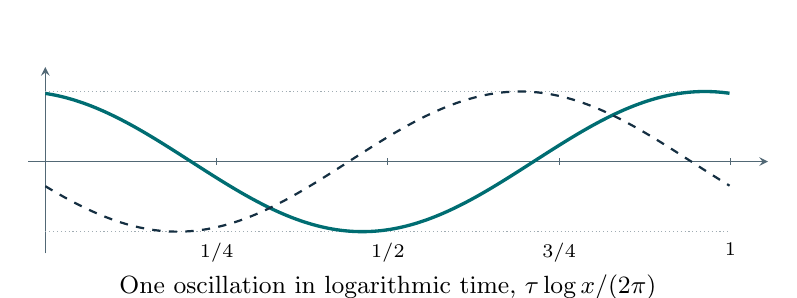
\begin{tikzpicture}[x=8.7cm,y=.89cm,>=stealth]
 \draw[->,quiet] (-.025,0)--(1.055,0);
 \draw[->,quiet] (0,-1.31)--(0,1.35);
 \foreach \x/\lab in {.25/{1/4},.5/{1/2},.75/{3/4},1/{1}}{
   \draw[quiet] (\x,.05)--(\x,-.05);
   \node[font=\scriptsize,anchor=north,fill=white,inner sep=1pt] at (\x,-1.12) {\(\lab\)};
 }
 \draw[densely dotted,quiet!55] (0,1)--(1,1) (0,-1)--(1,-1);
 \draw[very thick,accent,samples=96,domain=0:1,smooth]
     plot (\x,{cos(360*\x+atan(16/67))});
 \draw[thick,ink,dashed,samples=96,domain=0:1,smooth]
     plot (\x,{-cos(360*\x-atan(8/3))});
 \node[font=\small,anchor=north] at (.5,-1.47) {One oscillation in logarithmic time, \(\tau\log x/(2\pi)\)};
\end{tikzpicture}

\small\color{quiet}The solid curve is the model smoothed remainder and the dashed curve is the model sharp-count error. Each has been divided by its positive amplitude after removing its power of \(x\). The integral changes the phase as well as reversing the sign.
\end{center}

Finally the arithmetic estimate says \(R(x)\le x^{-1/2+\varepsilon}\) for each fixed good \(d\) and each positive \(\varepsilon\). Choose \(\varepsilon<\sigma-1/2\). Multiplying by \(x^{1-\sigma}\) makes the upper bound tend to zero, while \eqref{eq:analyticlab-excursion} requires a strictly positive upper limit. At the illustrative location \(3/4+2i\), the choice \(\varepsilon=1/8\) already separates the two powers. This conflict explains the role of all three ingredients at the endpoint. The twist isolates the multiplicity of the proposed zero. Positivity turns that multiplicity into an upward excursion. The long chain of theta lifts makes the admissible upper size of that excursion decay to zero.
At the boundary itself, the outcome is different. The elementary function
\[
       R_0(x)=x^{-1/2}\cos(\gamma\log x),\qquad \gamma>0,
\]
satisfies every upper bound \(R_0(x)\le x^{-1/2+\varepsilon}\) for \(x\ge1\). Its transform equals
\[
 \frac12\left(\frac{1}{s-1/2-i\gamma}
                  +\frac{1}{s-1/2+i\gamma}\right)
 \qquad (\Re s>1/2).
\]
It has a genuine pole at both indicated points of the critical line. This example distinguishes two places where a strict inequality is essential. The progression of test exponents may approach \(1/2\) arbitrarily closely. Each test reaches only the open half-plane to its right. The proof of equality of real parts uses the separate symmetry that confines a reflected zero from the other side as well.
\route{\sref{New/Reduction/OneSidedBound}{the eventual bound at each admissible prime}, \sref{Lib/Analytic/QuadraticTwist}{the choice of prime for a particular rectangle}}


\section{The statements and their verification}\label{sec:record}
The public interface has five theorems. In the table, each name links to its declaration in the vendored project. The four auxiliary proposition names in the source expand to formulas about Mathlib's functions. Their definitions import only Mathlib.
\begin{center}\renewcommand{\arraystretch}{1.18}
\begin{tabularx}{\linewidth}{@{}p{.48\linewidth}X@{}}
\toprule
\textbf{Lean theorem}&\textbf{Mathematical content}\\\midrule
\mainline{5}{\texttt{riemannHypothesis}} & Mathlib's proposition \texttt{RiemannHypothesis}.\\
\mainline{8}{\texttt{riemannZeta\_eq\_zero\_re}} & For a zero of \(\zeta\), exclude \(1\) and \(-2,-4,\ldots\). Its real part is \(1/2\).\\
\mainline{13}{\texttt{LFunction\_ne\_zero\_of\_half\_lt\_re}} & All moduli, all characters, \(\Re s>1/2\). Excludes the principal pole.\\
\mainline{17}{\texttt{LFunction\_eq\_zero\_re}} & Every zero in \(0<\Re s<1\) has real part \(1/2\), including for imprimitive characters.\\
\mainline{21}{\texttt{LFunction\_eq\_zero\_re\_of\_isPrimitive}} & The preceding assertion specialized to primitive characters.\\\bottomrule
\end{tabularx}\end{center}
A compact way to follow the dependency is to open the main inequality, which imports the short-forms and long-forms developments. The one-sided bound then imports that inequality together with the construction of admissible data, the fixed-modulus prime number theorem, and the zero-detection criterion. It exports \texttt{New.grh}. The functions that deduce \(\zeta\)-RH and Dirichlet zeros on the line each take the half-plane assertion as an argument. In the entry-point file this argument is filled by \texttt{New.grh}. Thus one can inspect the symmetry argument on its own and see exactly where the substantial arithmetic theorem is supplied.
\route{\sref{Statements}{definitions}, \sref{New/Reduction/OneSidedBound}{half-plane theorem}, \sref{New/Main}{conditional implications}, \sref{Main}{application}}

\subsection{Reading a proof term backward}
The top-level RH proof has essentially one line. In mathematical typesetting, its proof term reads
\[
 \texttt{New.zeta\_zeros\_on\_line}\quad\texttt{New.grh}.
\]
Juxtaposition means function application. The first term consumes a proof of half-plane nonvanishing and returns a proof of the zeta statement. The second supplies that input. Following the first name shows what follows from nonvanishing. Following the second shows how nonvanishing was obtained.

The table traces the second name back to the mathematical ingredients. It is ordered for a reader travelling \emph{upstream} from the conclusion. The references open the modules at the corresponding revision, and the accompanying source map gives declaration lines.
\begin{center}
{\small\renewcommand{\arraystretch}{1.19}
\begin{tabularx}{\linewidth}{@{}>{\raggedright\arraybackslash}p{.22\linewidth} >{\raggedright\arraybackslash}X >{\raggedright\arraybackslash}X@{}}
\toprule
\textbf{Question} & \textbf{What the source invokes} & \textbf{What to inspect}\\ \midrule
What excludes a zero? &
Choose \(Q=18480q\), move the character to that modulus, and apply the \sref{New/Reduction/Zeros/Criterion}{one-sided criterion}. &
In \sref{New/Reduction/OneSidedBound}{\texttt{grh}}, the point \(s=1\) is a separate case. The arithmetic input is quantified over the admissible primes.\\
Where does the power bound hold? &
\sref{New/Reduction/OneSidedBound}{\texttt{eventually\_\allowbreak primeRemainder\_\allowbreak le\_rpow}} passes from integer cutoffs to all sufficiently large reals. &
Follow the choice of the smaller exponent and the bound on the two remainders at \(x_1\).\\
Which volume enters? &
\sref{New/Reduction/MainInequality}{\texttt{star\_inequality}} chooses a basis from a union of images, bounds its index, then applies the lower estimate to it. &
The family \(y\) is the same in both inequalities. The variable \(n\) counts its members.\\
Where are the inputs? &
\sref{New/Reduction/ShortAndEnough}{Short integral forms and enough translates}; \sref{New/Determinant/Twist/LongForms}{long integral forms}. &
The upper theorem bounds lengths at each conjugate. The lower one bounds the covolume plus twice the index.\\
Where is the arithmetic read out? &
\sref{New/Reduction/PrimeSums}{\texttt{totalRemainder\_eq}} is a finite identity; \sref{New/Reduction/Zeros/PrimeError}{the transform theorem} reads its centered prime sums as poles. &
Check the minus sign on \(R_Q(x_1)\), the plus sign on \(R_1(x_1)\), and the opposite residues of the original and quadratic-twisted zeros.\\
\bottomrule
\end{tabularx}}
\end{center}

The directory \texttt{Lib/} supplies supporting theory, including analytic number theory, the Siegel--Weil and Rallis identities, and the Galois and local arithmetic used to control congruences. The directory \texttt{New/} arranges the constructions for these particular fields, weights and chains. The proof uses specialized versions of some broad theories. For example, trace information for a main summand and the prescribed cyclotomic string is used in the denominator argument. Understanding the assumptions of that precise statement is more informative here than invoking a general correspondence between all Galois and automorphic representations.

\subsection{Which source was analyzed}
The readable edition credits Levent Alpöge with Claude for the proof and Claude for the Lean text and project documents of the rewriting. This edition expands the supplied 60-page revised guide and follows the readable \texttt{grh/} package in Vladimir Reshetnikov's \emph{ProveIt}. The Git tree recorded in the vendored directory agrees with that in the original rewriting at the pinned commits below. The supplied guide pinned an earlier ProveIt revision (\texttt{438086c9}). We compared that revision and the ProveIt snapshot below. Both identify the readable directory by the same Git tree as the independently checked upstream edition. A Git tree identifies the directory entries and recursively their contents. The two directories therefore supply the same source for this exposition and for the published external check.
\begin{center}\small\renewcommand{\arraystretch}{1.12}
\begin{tabular}{@{}ll@{}}\toprule
\textbf{Object}&\textbf{Identifier}\\\midrule
\href{https://github.com/VladimirReshetnikov/ProveIt/tree/d8415e76ad850651f8c0083afe689dd9f4a45a10/Analysis/GeneralizedRiemannHypothesis/vendor/grh-lean}{ProveIt revision}&\texttt{d8415e76ad850651f8c0083afe689dd9f4a45a10}\\
\href{https://github.com/lsernau/grh-lean/tree/72fead102f663d5c7a407964a13dc0cf9d977207/grh}{Upstream revision}&\texttt{72fead102f663d5c7a407964a13dc0cf9d977207}\\
Readable \texttt{grh/} tree&\texttt{2e133df63d7f4da6b3059c4195324f8e9187ba73}\\
Lean toolchain&\texttt{v4.35.0}\\
Mathlib revision&\texttt{56a005855ea17e0b0958f73ec801ae140b0a1679}\\
\bottomrule\end{tabular}\end{center}
For this edition the public statements and selected proofs in the analytic, automorphic and Galois-theoretic argument were inspected against the pinned source. Each declaration indexed in the archive was located in the upstream checkout and each indexed file checked by its Git blob identifier. The mathematical argument is presented at the level of the estimates identified in each section. The Lean builds, independent proof-checker runs and statement comparisons reported below are Sutherland's published checks. This edition involved no new kernel replay.

\subsection{What was checked independently}
Andrew Sutherland's verification record for the exact upstream revision reports a sandboxed build of the readable edition and kernel replay of all 803 modules. Two machines produced identical solution exports. The paranoid Comparator run on the larger machine passed, and separate con-leche and con-ron comparisons matched all five statements against the challenge. The axiom output for each theorem contains only \texttt{propext}, \texttt{Classical.choice} and \texttt{Quot.sound}. These express propositional extensionality, classical choice and quotient soundness. The project supplies the number-theoretic argument in proof terms over this foundation. \href{https://math.mit.edu/~drew/shortgrh/}{Verification record}, \href{https://math.mit.edu/~drew/shortgrh/readable-axioms.log}{axiom output}, \href{https://math.mit.edu/~drew/shortgrh/readable-standalone-con-leche-compare.log}{statement-comparison log}.

The comparison uses a separate \texttt{Challenge.lean} which gives the expected theorem types and placeholders for their proofs. Comparator selects \texttt{Main} as its solution module. That module imports \texttt{New.Main} and supplies proofs that Comparator checks against the expected types. The placeholders belong to the challenge specification. The readable package has its own Lake project. Its build commands are run inside the vendored \texttt{grh/} directory. Reproduction commands for both the exposition and the Lean package are in the accompanying README.

Alpöge's announcement identifies the analogy with Stepanov's method and the decision to represent multiplicity by a sequence of lifts. The Lean FRO and Mathlib Initiative's joint statement concerns the original large proof of RH. The shorter readable rewriting used here has its own verification record as described above. \href{https://alpo.ge/remark.pdf}{Alpöge's account}, \href{https://leanprover-community.github.io/blog/posts/riemann-hypothesis/}{joint statement on the original}, \href{https://github.com/lsernau/grh-lean/tree/72fead102f663d5c7a407964a13dc0cf9d977207/grh}{readable edition}.

\subsection{Where to read next in the formalization}
For the shortest mathematical route, read the three files that define \(\mathcal R\), prove \eqref{eq:star}, and deduce \eqref{eq:oneside}, then open the zero criterion. To understand the arithmetic behind the sign, follow a local prime gain into the normalized short-form bound and compare it with the single-lift determinant ratio. The accompanying \texttt{source-index.html} groups 253 checked source references by section. The tabular version, \texttt{source-map.tsv}, gives the source path, line number and Git blob identifier for each. The example scripts reproduce finite calculations with exact arithmetic. The endpoint estimates in Section~\ref{sec:analyticlab} are deductions in this guide from the transform and positivity inputs. The upstream \href{https://github.com/lsernau/grh-lean/blob/72fead102f663d5c7a407964a13dc0cf9d977207/grh/GUIDE.md}{reading guide} supplies the conventions for the remaining modules.
\subsection{Primary sources for the ideas}

\begin{description}\setlength{\itemsep}{3pt}
\item[The original argument.] Levent Alpöge's four-page announcement gives the discovery sequence, including the finite-field analogy, the suggestion to take roughly \(\sqrt{x}\) lifts, and the intermediate cost calculation. Its chronology is the source for the historical attributions in Section~\ref{sec:discovery}. \href{https://alpo.ge/remark.pdf}{Announcement, pp.~1--4}.
\item[Finite-field multiplicity.] S.\ A.\ Stepanov's 1969 paper treats hyperelliptic curves over a prime field. E.\ Bombieri's Bourbaki exposé explains how to build an auxiliary function in the more general curve setting. \href{https://doi.org/10.1070/IM1969v003n05ABEH000834}{Stepanov}; \href{https://numdam.org/item/SB_1972-1973__15__234_0/}{Bombieri, exposé 430}.
\item[The earlier analytic criteria.] A.\ Weil's explicit formulas explain how a sum over zeros becomes a collection of local terms. M.\ Suzuki's weighted prime sums give a recent example in which eventual sign information already characterizes RH. Section~\ref{sec:analyticlab} compares the analytic hypotheses. \href{https://doi.org/10.1070/IM1972v006n01ABEH001866}{Weil}; \href{https://doi.org/10.1007/s11139-025-01238-9}{Suzuki}.
\end{description}


\clearpage
\section*{Notation at a glance}\phantomsection\label{sec:glossary}\addcontentsline{toc}{section}{Notation at a glance}
\begin{tabularx}{\linewidth}{@{}p{.19\linewidth}X@{}}
\toprule
\textbf{Symbol} & \textbf{Meaning in the argument}\\\midrule
\(q,\chi\)&The modulus and Dirichlet character in the final theorem.\\[3pt]
\(Q,d,\chi_d\)&The modulus used to test the remainder, an auxiliary prime in the class \(Q/2-1\), and its quadratic Dirichlet character. For the zero criterion use \(Q=18480q\).\\[3pt]
\(\psi,\xi_\iota\)&\(\psi\) ranges over all Dirichlet characters modulo \(Q\) in the logarithmic derivative. \(\xi_\iota\) is an auxiliary character of a unitary group used to control a local projection denominator.\\[3pt]
\(x,x_1,b,a\)&Target cutoff, distant cutoff, large ordinary weight, and special derivative order \(a=xb\). The variable \(y\) can denote a trial derivative order or a real argument of a remainder, as specified.\\[3pt]
\(E,\Phi,f\)&Auxiliary CM field, its places at infinity, and their number. A CM field is a totally imaginary quadratic extension of a totally real field.\\[3pt]
\(A,B,\kappa\)&Places with a special derivative, selected places of large ordinary weight, and the function recording ordinary weights.\\[3pt]
\(k,r,t,m\)&Initial source rank, initial target rank, rank increase on the \(Y\) side, and chain length.\\[3pt]
\(V,d_T,n\)&Target space of forms, its dimension, and size of the independent family used for the determinant comparison.\\[3pt]
\(s_\infty,s_{\rm fin}\)&Archimedean cost of a derivative, and its weighted sum of finite-prime gains.\\[3pt]
\(H,\mathcal R,R_u\)&Common main term, total excess over the special places, and smoothed arithmetic remainder in the class \(1\bmod u\).\\[3pt]
\(Z(\xi),\delta,V_0\)&Full chain Gram determinant, allowance for local index, and upper bound for the logarithmic squared covolume of the chosen family.\\\bottomrule
\end{tabularx}
\vspace{6pt}
\subsection*{Operations and terms used in the proof}
A \emph{jet} extracts Taylor data at the origin. In this construction it is the value \(P(\partial)F(0)\), where the polynomial \(P\) specifies a combination of partial derivatives.

A \emph{Hecke operator} sums translates indexed by arithmetic cosets. Its eigenvalues distinguish systems of forms. How closely eigenvalues from different systems agree modulo a prime affects the denominators of projections.

A \emph{period} of a form is an integral over a designated subgroup or quotient, often with a character as weight. Comparing such integrals relates the two paths of theta lifts. The period \emph{scale} \(\Omega\) appearing in \(s_\infty\) is a particular numerical normalization attached to the CM construction.


A \emph{finite place} records the size of the prime-ideal divisor of an algebraic number. A complex embedding gives an \emph{archimedean} size. Their joint constraint on a nonzero algebraic number is the product formula. An \emph{index} in this argument measures the finite-place cost of making a family integral. Its \emph{squared covolume} is the Gram determinant of the untwisted images.

The \emph{conductor} of a Dirichlet character is the least modulus from which it is induced. The conductor of an auxiliary twist likewise records its ramification. A \emph{residue} at a simple pole is the coefficient of \((s-z)^{-1}\). A \emph{residue class} modulo an integer is a congruence class; these are different uses of the word.

\end{document}
